\documentclass[10pt , a4paper]{report}
% The preceding line is only needed to identify funding in the first footnote. If that is unneeded, please comment it out.
% \usepackage[T2A,T1]{fontenc}
\usepackage{silence}
\usepackage{pmboxdraw}
\usepackage{cite}
\usepackage{amsmath,amssymb,amsfonts}
\usepackage{algorithmic}
\usepackage{graphicx}
\usepackage{listings}
\usepackage{textcomp}
\usepackage{sectsty}
\usepackage{xcolor}
\usepackage{appendix}
\def\BibTeX{{\rm B\kern-.05em{\sc i\kern-.025em b}\kern-.08em
    T\kern-.1667em\lower.7ex\hbox{E}\kern-.125emX}}

\usepackage[utf8x]{inputenc}
% \usepackage[english,russian]{babel}
\usepackage{cmap}

\usepackage{titlesec}
\titleformat{\chapter}
  {\normalfont\LARGE\bfseries}{\thechapter}{1em}{}
\titlespacing*{\chapter}{0pt}{3.5ex plus 1ex minus .2ex}{2.3ex plus .2ex}

%paragraphs params
\setlength{\oddsidemargin}{0cm}
\setlength{\textheight}{24cm}
\setlength{\textwidth}{16cm}
\setlength{\topmargin}{-2cm}
\renewcommand{\baselinestretch}{1.1}

% fonts
\usepackage{times}
\usepackage{helvet} 
\usepackage{sectsty}
\allsectionsfont{\sffamily}
\renewcommand{\familydefault}{\sfdefault}


%listings
\lstset{basicstyle=\ttfamily\footnotesize}
\lstset{frame=tlrb}
\usepackage{listings}

\usepackage{minted}
\usepackage{forest}

\usepackage{adjustbox}
\usepackage{subcaption}
\captionsetup{compatibility=false}

\newenvironment{code}{\captionsetup{type=listing}}{}

\setminted{
    breaklines=true,
    frame=single,
    framesep=5pt
}

\begin{document}

\title{Computer Science Project\\
        \textit{Kandy: CLI tool for managing Kafka}}

\author{\textbf{Alex Lukin}\\
Candidate number: 3643\\
Center number: 22109\\
Qualification code: H446 \\
Chesterton Community College\\
\textit{Cambridge, United Kingdom}\\}


\maketitle

\newpage
\tableofcontents
\newpage

\chapter{Analysis}
\section{Problem Definition}

Apache Kafka\footnote{\textbf{Kafka} is a distributed streaming platform designed for processing, storing, and transmitting data in real-time. It provides a reliable mechanism for data streaming, enabling applications and services to exchange information and respond to changes instantly. Kafka is built to handle enormous volumes of data, offering high performance and fault tolerance through its distributed architecture.} has become a crucial system for handling real-time data streams in today’s data-driven landscape. Despite Kafka’s widespread adoption, there remains a lack of streamlined tools for efficient management of Kafka instances directly from the command line. This gap poses a challenge for developers who need quick, straightforward ways to interact with Kafka without getting slowed down by complex setup processes.

While web applications can bridge this gap by providing intuitive interfaces, they are typically hosted in Docker containers. Docker’s benefits of portability and consistency across different environments are valuable, yet setting up these applications within large systems can become cumbersome and time-consuming, especially for quick local tests.

In summary, Docker facilitates deploying web applications with user-friendly interfaces for Kafka management, but its setup can be daunting within larger infrastructures. To address this, the proposed solution is a dedicated Text-Based User Interface (TUI) utility aimed at simplifying Kafka management, ultimately boosting developer productivity.

The project is named \textbf{Kandy}(Stands for Handy Kafka) and is envisioned as a TUI tool specifically designed for Kafka management

\section{Stakeholders} 
The Kandy project targets three primary stakeholder groups, each with distinct needs that Kandy will address:

\begin{itemize} 
    \item \textbf{Administrators} who oversee Kafka performance, data integrity, and cluster health. Kandy’s real-time monitoring features provide quick insights into cluster status, helping administrators maintain stability and react swiftly to any issues.
    \item \textbf{Developers} who integrate Kafka into their applications and require efficient access to Kafka for testing, debugging, and troubleshooting. Kandy streamlines access to critical metrics, enhancing their productivity and reducing setup time for Kafka-related tasks.
    \item \textbf{DevOps teams} responsible for Kafka cluster infrastructure, uptime, and stability. Kandy’s intuitive interface and essential monitoring tools enable DevOps teams to oversee cluster health without the need for complex GUI-based solutions, making management tasks more efficient.
\end{itemize}

To represent the target audience, I have identified a key user persona: \textbf{Sarah}, the Head of Engineering at Valerann. Sarah oversees multiple data-driven projects that rely on real-time Kafka streams, frequently monitoring consumer lags, topic performance, and system stability to ensure smooth operation for her teams. With extensive experience in both development and Kafka management, Sarah’s insights are invaluable for evaluating Kandy’s effectiveness. Sarah’s feedback will help me to be sure if Kandy meets the practical needs of it's users.

\newpage

\section{Kafka Architecture}\label{Kafka_architecture}

Throughout whole project, I will use terminology specific to Kafka’s architecture to describe its components and functionalities. So
this subsection dives into the foundational concepts of Kafka. For better understanding the key ideas behind Kafka and its functionality, let’s break it down into its core components and how they work together.

\begin{figure}[htbp]
    \centering
    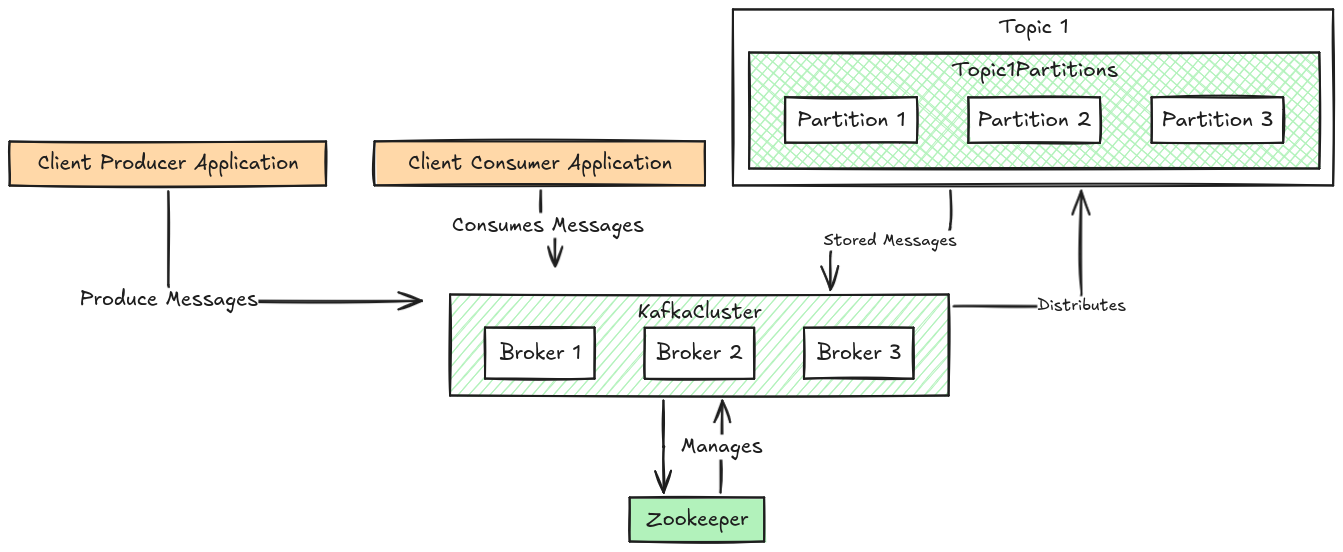
\includegraphics[width=1\linewidth]{imgs/KafkaStructureModel.png}
    \caption{Key Components of Kafka Architecture}
    \label{fig:kafka_arch}
\end{figure}

\subsubsection*{Core Components of Kafka}
\begin{itemize}
    \item \textbf{Message:} The fundamental unit of data in Kafka. It consists of a key, value, and optional metadata (headers)
    
    \textit{Example:} A message in the \textit{Weather\_Updates} topic might include a key representing a city ID, a value containing temperature data, and headers indicating the time of measurement.
    
    \item \textbf{Producers:}  
    These are the data generators. Producers are applications or systems responsible for sending messages to Kafka topics. Think of them as the "writers" in Kafka's ecosystem. 
    
    \textit{Example:} A weather monitoring application sending real-time temperature updates acts as a producer.

    \item \textbf{Consumers:}  
    Consumers retrieve and process data stored in Kafka topics. They are the "readers" that transform raw data into actionable insights or visualizations.  
    
    \textit{Example:} A live dashboard showing weather updates would be a consumer.

    \item \textbf{Topics and Partitions:}  
    \begin{itemize}
        \item \textbf{Topics:} Logical containers that organize messages by category. For instance, a topic named \textit{Weather\_Updates} might store all weather-related data.
        \item \textbf{Partitions:} Subsections of a topic that allow for parallel processing. Each partition stores messages in an immutable, sequential order. This setup enables Kafka to scale efficiently by distributing messages across multiple servers (brokers).
    \end{itemize}

    \item \textbf{Brokers:}  
    Brokers are Kafka's backbone. They store data and manage partitions. When combined, multiple brokers form a Kafka cluster, which offers high availability and fault tolerance by replicating and balancing data across servers.

    \item \textbf{Zookeeper:}  
    Zookeeper is a distributed coordination service crucial to Kafka's operations. It tracks metadata, manages partition leadership, and monitors broker health to ensure cluster stability. Although Zookeeper is essential in Kafka’s traditional setup, newer Kafka versions are moving towards its replacement with Kafka's internal \textit{KRaft} system.  
    \textit{(Note: I'm not planning on working with Zookeeper directly in this project, but understanding its role might be helpful)}
\end{itemize}

\subsubsection*{How Kafka Works}
\begin{enumerate}
    \item \textbf{Producers Generate Data:}  
    Applications acting as producers send data to Kafka, specifying the relevant topic. For instance, a weather app might publish updates to a \textit{Weather\_Updates} topic.

    \item \textbf{Kafka Distributes Data Across Partitions:}  
    Kafka divides incoming data into partitions within a topic and distributes these partitions across brokers in the cluster. This design allows efficient load balancing and supports simultaneous access by multiple consumers.

    \item \textbf{Consumers Process Data:}  
    Consumers subscribe to topics and retrieve data from specific partitions. Kafka ensures that data can be processed in parallel, enabling high-performance real-time analytics or other operations.
\end{enumerate}

\section{Computational Methods}

Managing Apache Kafka, a distributed and data-intensive system, requires careful application of computational methods. Kafka's complex architecture involves intricate interactions between brokers, topics, partitions, and consumers. Computational approaches simplify this complexity, making it feasible to develop a Text-Based User Interface (TUI) that provides users with an intuitive way to manage Kafka. This section outlines how principles such as \textit{Abstraction}, \textit{Decomposition}, \textit{Thinking Ahead}, and \textit{Algorithmic Thinking} are employed in the development of the TUI.

\subsection{Abstraction}

\subsubsection*{Definition:}  
Abstraction simplifies a complex system by emphasizing its essential features while hiding less relevant details.

\subsubsection*{Application:}  
Abstraction is at the heart of this TUI’s design, allowing users to interact with Kafka’s core components—brokers, topics, partitions, and consumer groups—without requiring deep knowledge of Kafka’s APIs or internal mechanisms. The TUI abstracts Kafka’s functionalities into high-level commands and representations:
\begin{itemize}
    \item \textbf{Brokers:} Represented as nodes with health status and connectivity information.
    \item \textbf{Topics:} Abstracted as logical containers for message streams, with partition and replication details available upon request.
    \item \textbf{Consumers:} Displayed as groups subscribing to topics, with key metrics such as consumer lag simplified for clarity.
\end{itemize}

This abstraction ensures that even novice users can perform critical Kafka operations, such as topic creation, monitoring, and deletion, using an accessible interface.

\subsection{Decomposition}

\subsubsection*{Definition:}  
Decomposition breaks a large, complex problem into smaller, manageable sub-problems.

\subsubsection*{Application:}  
The development of the TUI leverages decomposition to divide Kafka management into specific functional components:
\begin{itemize}
    \item \textbf{Topic Management:} Includes operations such as creating, deleting, and listing topics with detailed configurations.
    \item \textbf{Consumer Monitoring:} Tracks consumer groups, displays subscription details, and monitors consumer lag.
    \item \textbf{Broker Status Monitoring:} Reports on broker health and displays connectivity details.
\end{itemize}

Each component is further divided into smaller tasks. For example, ``Topic Management'' includes sub-tasks like validating topic names, setting replication factors, and handling partition assignments. Decomposition makes the project more manageable, enables iterative development, and allows for parallelization of work across different modules.

\subsection{Thinking Ahead}

\subsubsection*{Definition:}  
Thinking Ahead involves anticipating future needs and ensuring the solution is robust and scalable.

\subsubsection*{Application:}  
The TUI is designed with extensibility in mind, anticipating potential changes in Kafka’s architecture and user requirements. For instance:
\begin{itemize}
    \item The TUI supports dynamic configuration, allowing it to adapt to changes in the number of brokers or topics without significant modifications.
    \item Modular code design ensures that new features, such as support for Kafka Streams or advanced monitoring tools, can be integrated seamlessly.
\end{itemize}

By thinking ahead, the TUI ensures long-term usability and minimizes maintenance efforts, even as Kafka evolves.

\subsection{Algorithmic Thinking}

\subsubsection*{Definition:}  
Algorithmic Thinking involves designing and implementing efficient, logical steps to solve a problem.

\subsubsection*{Application:}  
Several features of the TUI rely on algorithmic thinking:
\begin{itemize}
    \item Efficient algorithms for calculating consumer lag ensure that real-time metrics are displayed without significant delays.
    \item Partition assignment algorithms optimize how messages are distributed across brokers, ensuring load balancing.
    \item Sorting and filtering operations in the TUI enable users to quickly locate relevant topics or consumers, even in large Kafka clusters.
\end{itemize}

These algorithmic enhancements ensure that the TUI provides accurate and responsive feedback, critical for managing a live distributed system.

\subsection{Evaluation and Refinement}

As part of the computational process, evaluation and refinement ensure that the TUI meets user needs effectively. Continuous testing is performed to verify:
\begin{itemize}
    \item Usability: Ensuring the interface remains intuitive for users with varying levels of experience.
    \item Performance: Verifying that the TUI scales efficiently with large Kafka clusters.
    \item Correctness: Ensuring that operations, such as topic creation or consumer monitoring, produce accurate results.
\end{itemize}

\subsection{Conclusion}

By applying computational methods such as abstraction, decomposition, thinking ahead, and algorithmic thinking, the TUI simplifies Kafka management for users. These principles ensure that the solution is user-friendly, scalable, and adaptable to future requirements, demonstrating the importance of computational methods in solving complex, real-world problems.


\chapter{Research}
\section{Interview questions}

I will outline here key questions that I will ask stakeholder, but during the interview I may come up with follow up questions. The interview will help me find their opinion on the software and how they would like to use it.

\subsection{Questions}
\begin{itemize}
    \item \textbf{How often do you work with Kafka? What utilities do you use to work with it? Why those?}
        \begin{itemize}
            \item Understanding the frequency of interaction with Kafka is crucial for designing a utility that meets the stakeholder's needs without overwhelming them with unnecessary features
        \end{itemize}
    \item \textbf{Can you describe in detail the last problem you solved related to Kafka?}
    \begin{itemize}
            \item Gathering detailed information about recent challenges helps in designing features and functionalities within the utility to address common pain points
    \end{itemize}
    \item \textbf{Is there anything you're currently dissatisfied with in the utilities you use? What would you change?}
        \begin{itemize}
            \item Discovering dissatisfaction with existing utilities guides the development of the utility by focusing on areas for improvement or enhancement
            \item Knowing desired changes informs feature prioritisation, ensuring that the utility aligns with stakeholder expectations and addresses their specific pain points effectively
        \end{itemize}
    \item \textbf{Do you have a preference for a Terminal User Interface (TUI) or web-based solution for managing Kafka? If so, what are the reasons behind your preference?}
        \begin{itemize}
            \item Understanding stakeholders' preferences for either a Terminal User Interface or web-based solution provides crucial insights into their workflow preferences and the environment in which they operate. This information ensures that the utility is developed in a manner that seamlessly integrates into their existing workflows, ultimately enhancing user experience and satisfaction
        \end{itemize}
    \item \textbf{Describe the recent problems you encountered while using <Name of the utilities>}
        \begin{itemize}
            \item Identifying areas of dissatisfaction with current utilities allows for targeted improvements in the design and functionality of the TUI utility. By addressing these pain points, the TUI utility can be tailored to better meet the needs and expectations of stakeholders, resulting in a more effective and user-friendly solution.
        \end{itemize}
        
    \item \textbf{What do you believe would be the ideal number of clusters the system should handle simultaneously? Why? How many clusters have you worked with simultaneously in the past?}
        \begin{itemize}
            \item Understanding the optimal number of clusters for concurrent support is key to ensuring the system scales seamlessly and manages resources efficiently.
        \end{itemize}
    \item \textbf{Could you explain how you currently configure connections to the clusters, and how user-friendly do you find this process?}
        \begin{itemize}
            \item Understanding how connections to the clusters are currently configured and evaluating the user-friendliness of this process can provide valuable insights, ensuring that the new utility addresses any shortcomings and provides a seamless user experience.
        \end{itemize}
    \item \textbf{When thinking about how data from the clusters is displayed, what are your main expectations? For example, how quickly data is presented by current tools, and how satisfied are you with this?}
        \begin{itemize}
            \item Understanding the expectations regarding data display from the clusters is crucial for informing development priorities and ensuring alignment with stakeholder needs and by gaining insights into these aspects, we can effectively prioritise features and enhancements within the utility
        \end{itemize}
    \item \textbf{Can you describe some common scenarios where you would use multiple clusters? For instance, comparing data across different topics or any other important scenarios you have in mind?}
        \begin{itemize}
            \item Understanding common scenarios where users would use multiple clusters is important for designing a utility that meets users’ needs effectively. By considering these scenarios, I can ensure that the utility is versatile enough to support a wide range of users workflow needs
        \end{itemize}
\end{itemize}


\section{Interview}


\subsection*{Can you please introduce yourself and describe your experience with Kafka?}

Sure. My name is Sarah Anderson, and I’m the Head of Engineering at Valerann. I’ve been with the company for nearly three years, and I’ve been working in tech for almost ten years. Regarding my experience with Kafka, I started using it about six years ago while working at a marketing technology company. They used Kafka to process large volumes of email notifications and automatically convert them into sales. Since then, I’ve worked with Kafka in about five different companies, all primarily for high-volume, real-time data processing.

Typically, my role with Kafka has involved helping companies implement and scale it from the ground up. Kafka provides excellent scalability, but transitioning from a traditional monolithic architecture to an event-driven, Kafka-based design requires significant effort. Developers often need training, and management needs to understand how to structure and scale a Kafka architecture. I’ve spent much of my time helping teams learn how to use Kafka, build systems around it, and implement it effectively.

\subsection*{How often do you work with Kafka now, and what utilities and tools do you use to manage it?}

Currently, I work with Kafka every few days—around three times a week. However, I don’t interact with the individual services as much as I used to. In terms of tools, we primarily use a tool called Faust Streaming, which was derived from an older tool called Faust (created by a company called Robinhood, not to be confused with the Bitcoin company). However, Faust is now deprecated, and we’re moving away from it. We’ve been using it as our streaming framework, similar to the Kafka Streams Java framework but written in Python—and not as efficiently. We're gradually replacing it with an in-house tool we’ve developed called CitizenK (inspired by the movie \textit{Citizen Kane} and Kafka's initial).

For managing Kafka day-to-day, we use an open-source tool from Provectus Labs that provides a free UI for administering Kafka clusters, performing tasks like cleaning up consumer groups or resetting offsets. For infrastructure management, we use Terraform to create clusters, brokers, topics, and set up initial settings.

\subsection*{Can you describe any problems you've encountered while using these tools to manage Kafka?}

One of the most common issues we face with admin tools is the lack of effective consumer group management. No tool I've found manages consumer groups as well as the Kafka CLI, but the CLI is cumbersome to use on a daily basis since it requires running bash scripts. For example, if you want to remove a topic from a consumer group, no admin tool I know of can do that; they only allow you to delete the entire consumer group or reset offsets. The CLI supports this, but no admin tool does, which is frustrating.

\subsection*{Do you prefer web tools over CLI tools? Why?}

I prefer web tools because they make onboarding new users much easier. It's harder to get people to read through extensive documentation to learn CLI tools. With a web interface, you can include visual guides like screenshots with instructions such as "click this button," which is much more intuitive. Writing documentation for CLI usage, such as which arguments to use and when, is far more complex. Admin UIs also offer the ability to limit user permissions, which is helpful. For example, tools like Conductor allow you to create user accounts with different levels of permissions, whereas with the CLI, users can do almost anything once they have access.

\subsection*{Would you prefer a Terminal User Interface, like Lazydocker, or a Web Interface?}

Personally, I prefer a web interface, although I know many developers prefer terminals. I’m one of the rare developers who enjoys working with a web interface. However, a terminal interface could benefit many people, especially if it’s easier to use than the Kafka CLI. A simplified terminal interface that eliminates the need to reference various configuration files and allows everything to be executed from a single root command would be a vast improvement.

\subsection*{Can you describe your experience working with multiple Kafka clusters simultaneously?}

We currently have seven Kafka clusters, each with both staging and production environments, which are differentiated only by name. Managing these clusters can be challenging. It would be great to have a tool that allows you to scan messages across all clusters or filter topics across clusters. Managing consumer groups across multiple clusters is also a manual process. For instance, resetting the offset of a consumer group in every cluster requires going through each cluster one by one, which is time-consuming and error-prone.

\subsection*{How do you connect to Kafka clusters, and how user-friendly is the process?}

We connect to Kafka clusters in three main ways. First, for all our services running in AWS, we use an AWS secret that contains Kafka credentials. These credentials are global, shared across all services for a particular customer. This makes things easier, although we recognize that creating separate credentials per service is something we should do but haven’t yet automated.

Second, we use an admin UI, which runs on local machines rather than in the cloud. We have an internal CLI tool that starts the Kafka UI, reconnecting it to all our clusters so we can browse them through the interface.

Third, we interact with Kafka through the CLI. We have another internal CLI tool that generates Kafka configuration files using the AWS global secret.

\subsection*{What are your expectations for how data from clusters, such as topics and consumer groups, should be displayed?}

I think flexibility is key. It would be great to customize the way data is displayed, for example, by pulling out information for a specific topic across all clusters or viewing all topics for a particular cluster. Additionally, showing statistics like the minimum and maximum lag for a particular topic across clusters, or the average size of topics, would be very useful.

\subsection*{Are you satisfied with the current tools’ representation of this data?}

No, I’m not satisfied at all. Most tools are awkward to use. They typically have separate subsections for topics and consumer groups, but navigating between them is cumbersome, and you often lose track of where you are in the interface.

\subsection*{Can you describe the last Kafka-related problem you solved?}

The last Kafka-related problem I solved was deleting topics and consumer groups. Since we use Amazon MSK to host Kafka, AWS handles most of the Kafka-specific issues that arise from maintaining clusters. Our biggest challenges are usually administrative, like keeping Kafka topics up-to-date as we change their structure and settings.

\subsection*{How important is it to sort topics by different parameters in your daily tasks?}

It would be extremely useful to sort topics by parameters like message volume or data size. Many of our services share topics, so sometimes, a service will start producing a large number of messages to a shared topic. Being able to quickly identify which topics have the highest message count or data volume would help us stay on top of this. Unfortunately, our current admin UI only allows us to sort topics by name, which isn’t very helpful.

\subsection*{What are the top three features you’d like to see in a Kafka admin UI tool?}

\begin{itemize}
    \item Better management of consumer groups that supports all the features available in the Kafka CLI.
    \item Cross-cluster topic statistics, so we can compare topics across multiple clusters and see metrics like size, number of connections, etc.
    \item The ability to limit user permissions. For instance, I don’t want everyone to be able to delete topics; only a few people should have that capability. It would be helpful if the UI could enforce this, in addition to Kafka’s own security settings.
\end{itemize}

\textbf{Insights from Interviews}: Key needs identified include comprehensive consumer group management, cross-cluster statistics, and user permissions. These priorities will directly inform Kandy’s development, focusing on user-centered functionality improvements.
\newpage
\section{Research on Existing Solutions}

To develop an effective Kafka management tool that aligns with the needs of Kafka administrators and engineers, I conducted a research of existing solutions across GitHub, Habr, Reddit threads focused on Kafka, and various package repositories. This research aimed to identify current tools’ strengths and limitations, assess their suitability for a secure, scalable environment.

\subsection{Criteria for Evaluating Usability}
To assess each tool's effectiveness, I developed the following criteria, informed by Sarah’s preferences and project objectives

\begin{enumerate}
    \item \textbf{Open Source}: Determines the ability to customize and scale the tool affordably in an enterprise environment.
    \item \textbf{Cost}: Evaluates cost-effectiveness for deployment at scale, balancing proprietary options against open-source flexibility.
    \item \textbf{Interface Type}: The tool’s user interface—CLI, TUI, or web-based—affects usability, with a preference for web-based tools for accessibility and TUI for optional flexibility.
    \item \textbf{Consumer Group Management}: Ability to manage consumer groups, including tasks like targeted offset resets, affects the tool's effectiveness in data-driven operations.
    \item \textbf{Cross-Cluster Capabilities}: Supports management across multiple Kafka clusters, vital for Sarah’s team managing complex deployments.
    \item \textbf{Data Sorting and Flexibility}: Ability to sort topics by message volume, data size, and other metrics for an optimized user experience.
    \item \textbf{User Permissions}: Provides secure, granular user roles for safe, role-based access management in multi-user environments.
\end{enumerate}

\newpage

\subsection{Kafka Manager} 
\subsubsection*{Overview} 
Kafka Manager, a community-maintained open-source tool by Yahoo, offers a basic web-based interface for managing Kafka clusters. It provides standard functionality for topic visibility and consumer group management.

\paragraph{Features and Limitations Based on Criteria}
\begin{itemize} 
    \item \small \textbf{Open Source}: Yes
    \item \small \textbf{Cost}: Free 
    \item \small \textbf{Interface Type}: Web 
    \item \small \textbf{Consumer Group Management}: Limited; lacks granular control such as the ability to remove specific topics from a consumer group, an important feature for custom data pipelines.
    \item \small \textbf{Cross-Cluster Capabilities}: Lacks multi-cluster management; suitable only for single-cluster setups, making it less viable for larger, distributed teams.
    \item \small \textbf{Data Sorting and Flexibility}: Limited sorting options; topics are sortable by name only, which restricts dynamic data organization.
    \item \small \textbf{User Permissions}: Lacks user-role management, posing a security concern in multi-user environments.
\end{itemize}

\begin{figure}[htbp]
  \begin{center}
    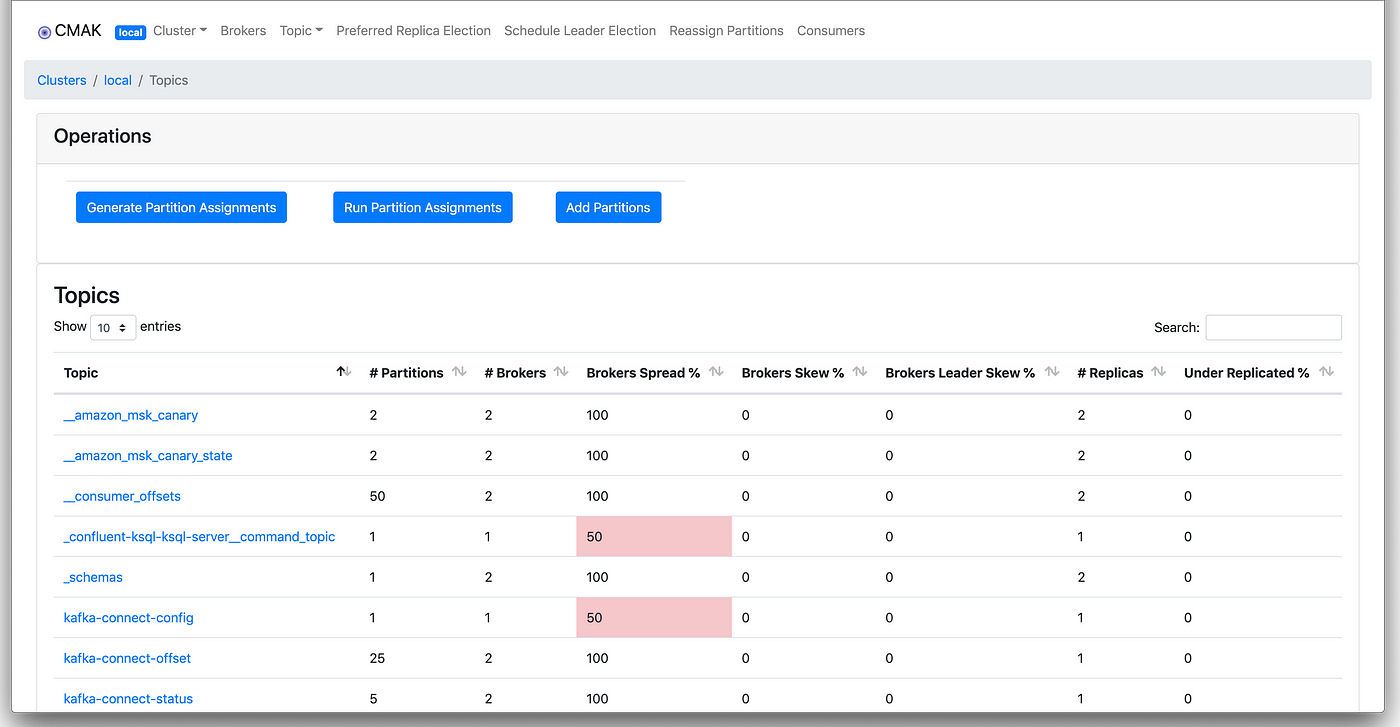
\includegraphics[width=0.95\textwidth]{imgs/KafkaManager.png}
  \end{center}
  \caption{}\label{fig:}
\end{figure}


\textbf{Suitability Summary}: Kafka Manager’s lack of cross-cluster capabilities and limited consumer group control reduce its practicality for Sarah’s team. Its single-cluster design makes it less scalable, while the absence of user permissions limits security. I like how UI arranged and probably will base my own solution on the similar design

\subsection{Conduktor} 
\subsubsection*{Overview} 
Conduktor, a proprietary Kafka management tool, offers a robust web-based GUI with advanced querying capabilities. Its features cater to a broad range of Kafka ecosystem components, providing operators with enhanced flexibility.

\paragraph{Features and Limitations Based on Criteria}
\begin{itemize} 
    \item \small \textbf{Open Source}: No
    \item \small \textbf{Cost}: Proprietary; requires licensing, which may reduce cost-effectiveness at scale.
    \item \small \textbf{Interface Type}: Web
    \item \small \textbf{Consumer Group Management}: Provides good consumer group controls but lacks the granularity found in CLI tools for highly specific data manipulation.
    \item \small \textbf{Cross-Cluster Capabilities}: Supports multiple clusters but lacks cross-cluster statistics, which limits data insights across clusters.
    \item \small \textbf{Data Sorting and Flexibility}: Offers flexible sorting by various metrics; however, it does not support cross-cluster topic comparisons, limiting use in environments needing aggregated insights.
    \item \small \textbf{User Permissions}: Includes role-based access controls, a core requirement for Sarah’s team.
\end{itemize}

\begin{figure}[htbp]
  \begin{center}
    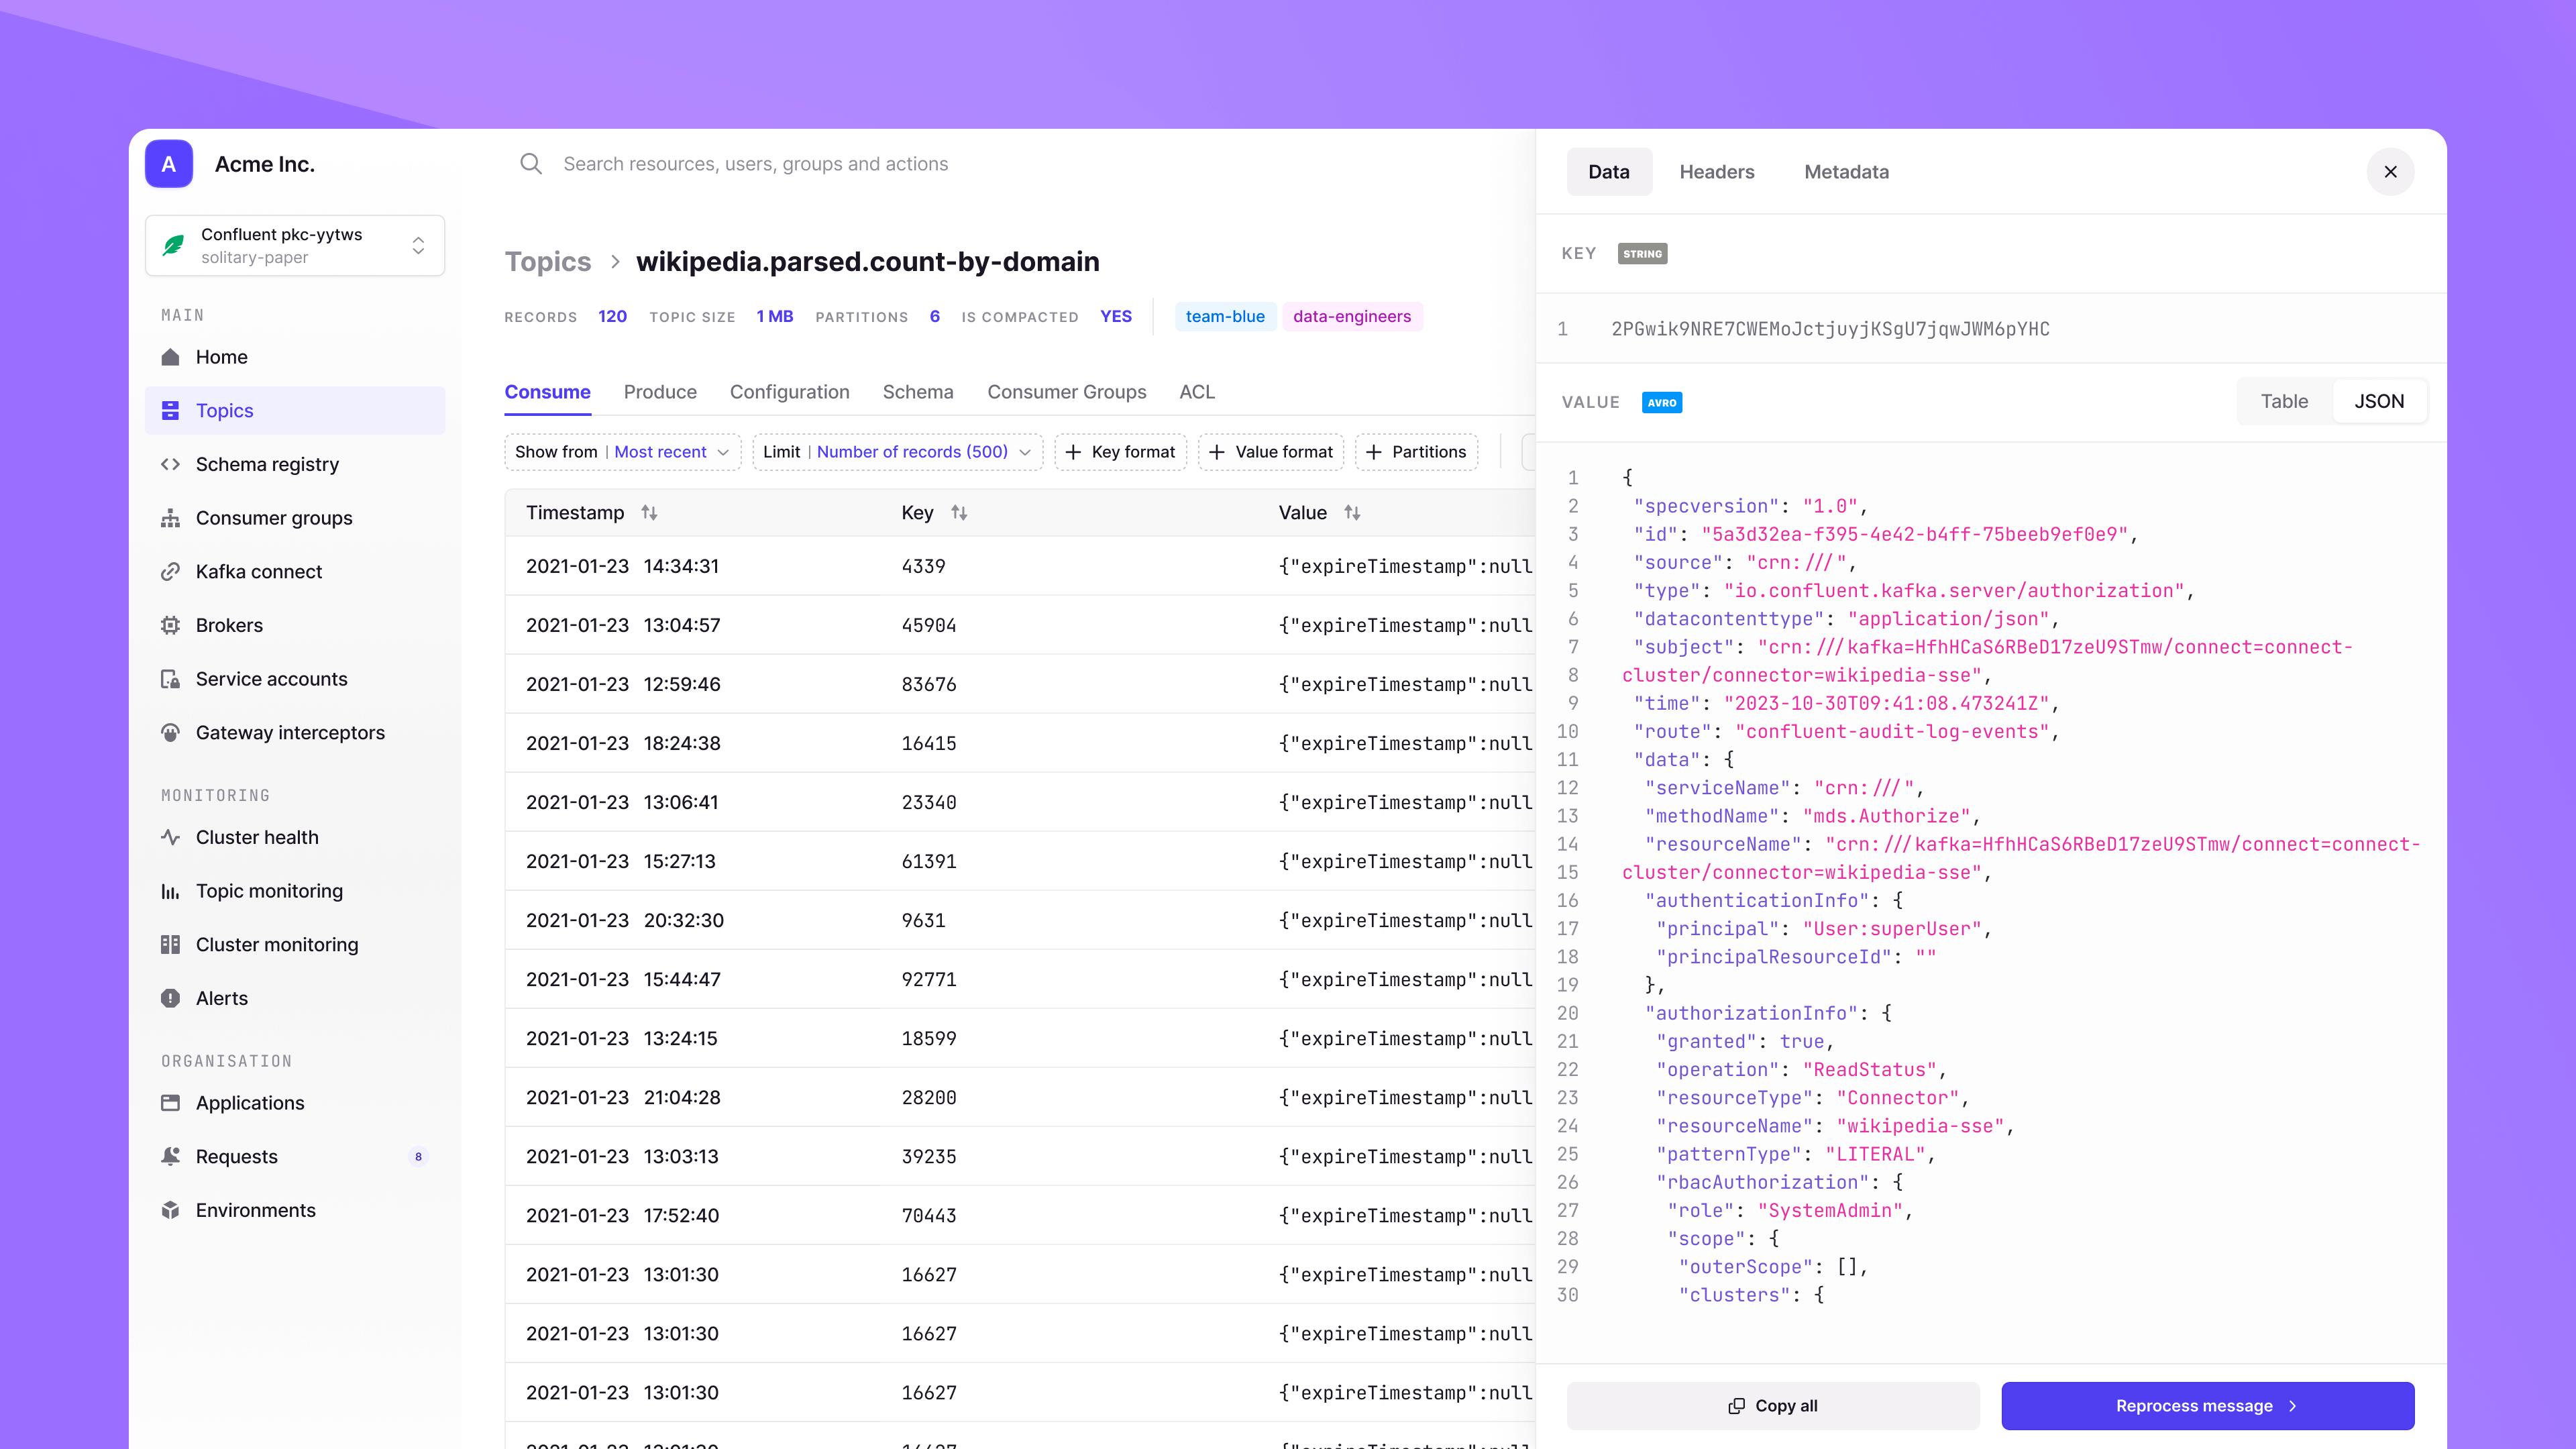
\includegraphics[width=0.95\textwidth]{imgs/Conduktor.png}
  \end{center}
  \caption{}\label{fig:}
\end{figure}


\textbf{Suitability Summary}: Conduktor’s robust interface and user-permission management are valuable; however, its proprietary model and limited cross-cluster statistics make it less adaptable for scalable, cost-effective deployments. This is comment from the developer. that works with Sarah, as I didn't really have chance to touch Conductor due it's price

\subsection{Kafdrop} 
\subsubsection*{Overview} 
Kafdrop is an open-source, web-based tool for monitoring Kafka clusters. It provides a straightforward UI, focusing on Kafka brokers, topics, and partitions, making it suitable for small to medium clusters.

\paragraph{Features and Limitations Based on Criteria}
\begin{itemize} 
    \item \small \textbf{Open Source}: Yes
    \item \small \textbf{Cost}: Free
    \item \small \textbf{Interface Type}: Web
    \item \small \textbf{Consumer Group Management}: Basic; lacks advanced control such as offset resets for specific consumer groups.
    \item \small \textbf{Cross-Cluster Capabilities}: Not supported; limited to monitoring single clusters.
    \item \small \textbf{Data Sorting and Flexibility}: Limited sorting options; cross-cluster comparisons absent.
    \item \small \textbf{User Permissions}: Does not support role-based access control, which reduces its security in multi-user scenarios.
\end{itemize}

\begin{figure}[htbp]
  \begin{center}
    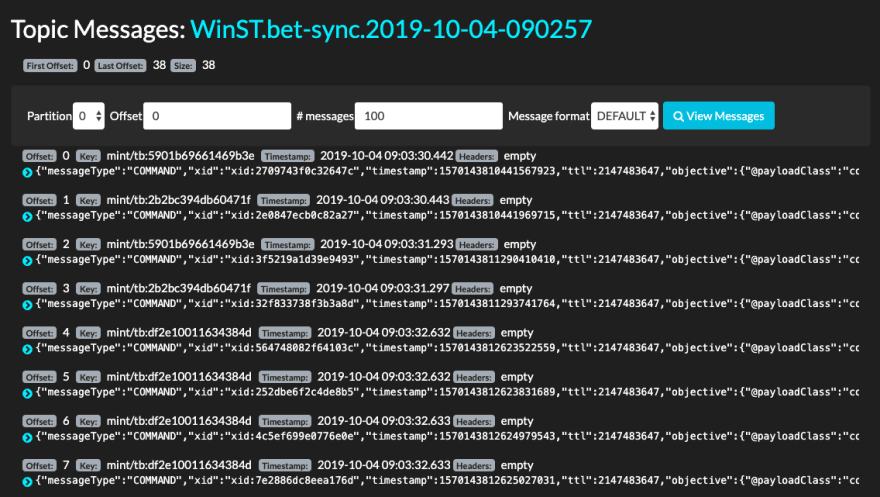
\includegraphics[width=0.95\textwidth]{imgs/Kafdrop.png}
  \end{center}
  \caption{}\label{fig:}
\end{figure}


\textbf{Suitability Summary}: While user-friendly, Kafdrop’s limited features make it unsuitable for large-scale Kafka operations, especially those requiring in-depth consumer group management and cross-cluster capabilities.

\subsection{Kafka CLI Tools} 
\subsubsection*{Overview} 
Kafka CLI Tools, built directly into Apache Kafka, provide a set of powerful, low-level commands for various management tasks, including managing topics and consumer groups.

\paragraph{Features and Limitations Based on Criteria}
\begin{itemize} 
    \item \small \textbf{Open Source}: Yes
    \item \small \textbf{Cost}: Free
    \item \small \textbf{Interface Type}: CLI
    \item \small \textbf{Consumer Group Management}: Comprehensive; provides granular control over offsets, including removing specific topics from consumer groups.
    \item \small \textbf{Cross-Cluster Capabilities}: Limited; each cluster requires manual configuration.
    \item \small \textbf{Data Sorting and Flexibility}: Limited; lacks built-in sorting and visualization without custom scripting.
    \item \small \textbf{User Permissions}: No user-role management, complicating restricted access in shared environments.
\end{itemize}

\begin{figure}[htbp]
  \begin{center}
    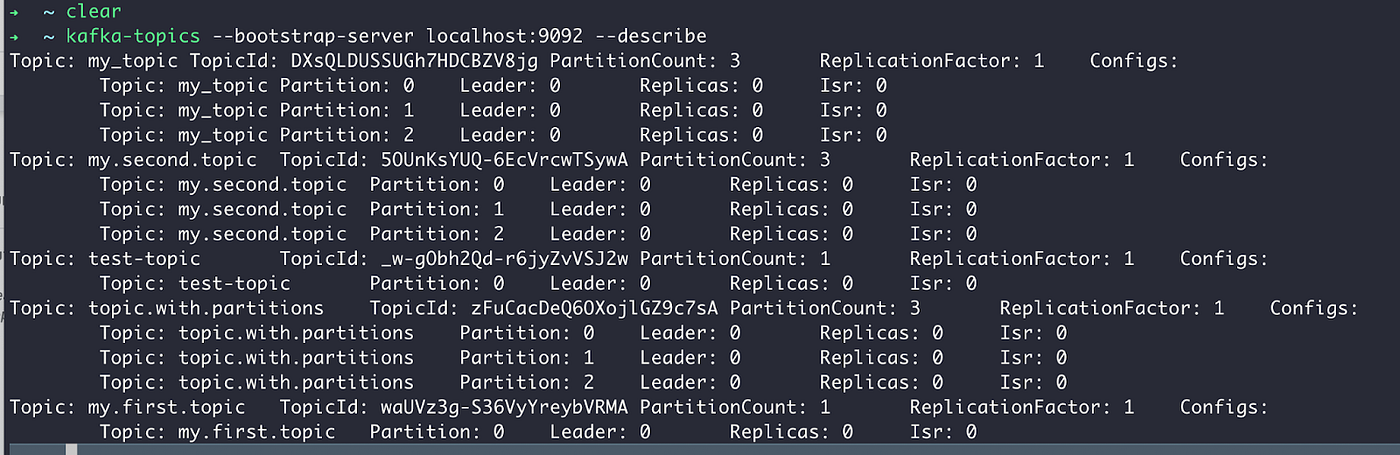
\includegraphics[width=0.95\textwidth]{imgs/KafkaCLI.png}
  \end{center}
  \caption{}\label{fig:}
\end{figure}


\textbf{Suitability Summary}: Kafka CLI Tools provide high control but lack usability for daily operations, visualizations, and multi-user management, making them unsuitable for teams requiring intuitive interfaces and cross-cluster management.

\subsection{kafkactl} 
\subsubsection*{Overview} 
kafkactl, an open-source CLI tool inspired by Kubernetes’ \texttt{kubectl} syntax, is designed for teams familiar with Kubernetes looking to streamline Kafka management.

\paragraph{Features and Limitations Based on Criteria}
\begin{itemize} 
    \item \small \textbf{Open Source}: Yes
    \item \small \textbf{Cost}: Free
    \item \small \textbf{Interface Type}: CLI
    \item \small \textbf{Consumer Group Management}: Moderate; lacks full Kafka CLI capabilities.
    \item \small \textbf{Cross-Cluster Capabilities}: Not inherently supported; can be configured.
    \item \small \textbf{Data Sorting and Flexibility}: Limited; requires additional scripting for data sorting.
    \item \small \textbf{User Permissions}: No role-based management, limiting security in multi-user settings.
\end{itemize}

\begin{figure}[htbp]
  \begin{center}
    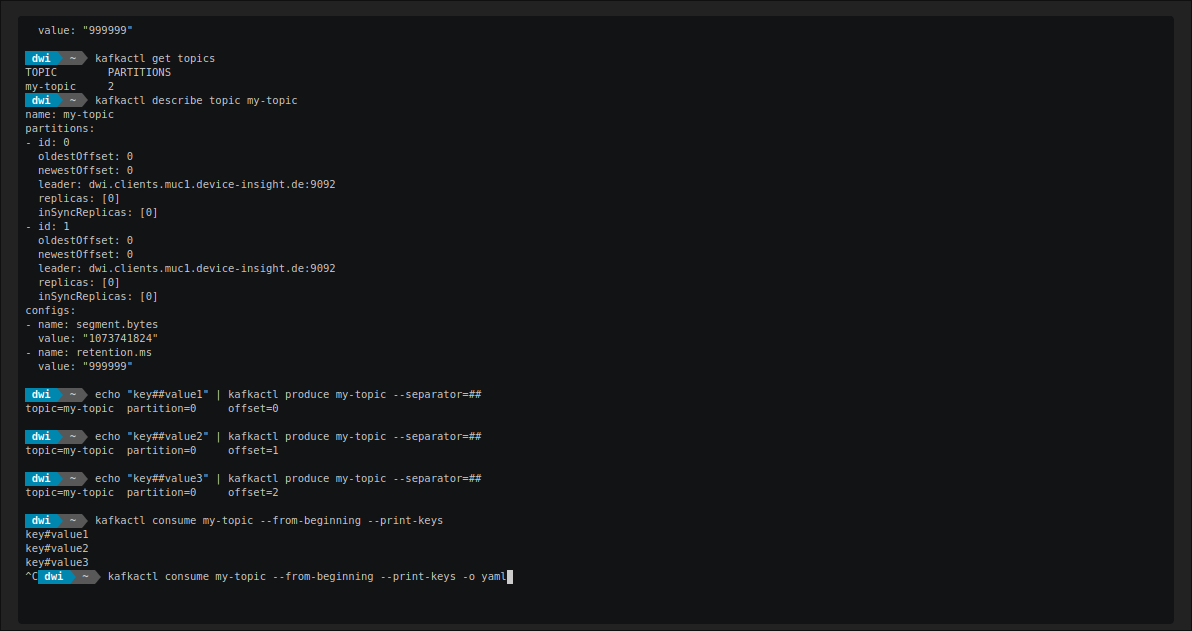
\includegraphics[width=0.95\textwidth]{imgs/Kafkactl.png}
  \end{center}
  \caption{}\label{fig:}
\end{figure}


\textbf{Suitability Summary}: kafkactl is more suited to teams with existing CLI expertise but lacks essential user permissions and cross-cluster capabilities for complex deployments.

\subsection{Kafka Monitor} 
\subsubsection*{Overview} 
Kafka Monitor, an open-source tool by LinkedIn, provides monitoring for Kafka performance, primarily focusing on end-to-end latency, throughput, and reliability.

\paragraph{Features and Limitations Based on Criteria}
\begin{itemize} 
    \item \small \textbf{Open Source}: Yes
    \item \small \textbf{Cost}: Free
    \item \small \textbf{Interface Type}: CLI-based monitoring
    \item \small \textbf{Consumer Group Management}: Limited; primarily a monitoring tool.
    \item \small \textbf{Cross-Cluster Capabilities}: Lacks cross-cluster monitoring.
    \item \small \textbf{Data Sorting and Flexibility}: Primarily focused on performance metrics with minimal interactive sorting.
    \item \small \textbf{User Permissions}: No role management, limiting secure multi-user access.
\end{itemize}

\begin{figure}[htbp]
  \begin{center}
    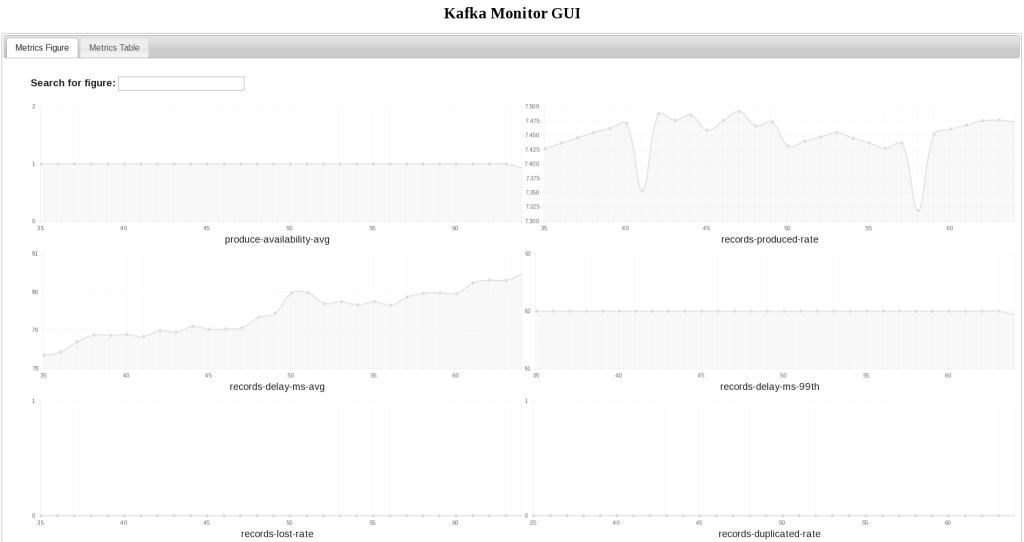
\includegraphics[width=0.95\textwidth]{imgs/KafkaMonitor.png}
  \end{center}
  \caption{}\label{fig:}
\end{figure}


\textbf{Suitability Summary}: While beneficial for performance monitoring, Kafka Monitor lacks management and cross-cluster features needed for daily Kafka administration.

\newpage
\subsection{Comparative Summary}

\begin{table}[h]
\centering
\resizebox{\textwidth}{!}{%
\begin{tabular}{|l|c|c|c|c|c|c|c|}
\hline
\textbf{Tool} & \textbf{Open Source} & \textbf{Cost} & \textbf{Interface} & \textbf{Consumer Group} & \textbf{Cross-Cluster} & \textbf{Data Sorting} & \textbf{Permissions} \\ \hline
Kafka Manager & Yes & Free & Web & Limited & No & Minimal & No \\ \hline
Conduktor & No & Proprietary & Web & Good & Limited & Flexible & Yes \\ \hline
Kafdrop & Yes & Free & Web & Basic & No & Minimal & No \\ \hline
Kafka CLI Tools & Yes & Free & CLI & Comprehensive & Manual & Minimal & No \\ \hline
kafkactl & Yes & Free & CLI & Moderate & Configurable & Limited & No \\ \hline
Kafka Monitor & Yes & Free & CLI & Limited & No & Minimal & No \\ \hline
\end{tabular}%
}
\caption{Comparison of Kafka Management Tools by Feature}
\end{table}

After gathering this information, it’s evident that Conduktor largely addresses Sarah's requirements.\footnote{As I later learned, \textbf{Conduktor} is indeed the solution Sarah's team uses in their development process.} It would be ideal to explore its functionality further; however, due to its proprietary nature, I was unable to do so.

The next best options to consider for development are Kafka CLI Tools and Kafka Manager. Kafka CLI Tools were developed by Confluent, the creators of Kafka, and offer a full suite of utilities to manage Kafka-related issues. However, based on Sarah's feedback and my own experience, Kafka CLI Tools can be challenging to use due to the numerous commands and flags, which are not always intuitive. Kafka Manager, on the other hand, is a free alternative to Conduktor, supporting all essential features needed for cluster management. 

\newpage
\section{Look into Other TUI Applications}

My experience in UI development is close to zero, so I decided to draw inspiration and knowledge from TUI wrappers for other services, such as:

\textbf{lazydocker}: A TUI for managing Docker containers

\begin{figure}[htbp]
    \centering
    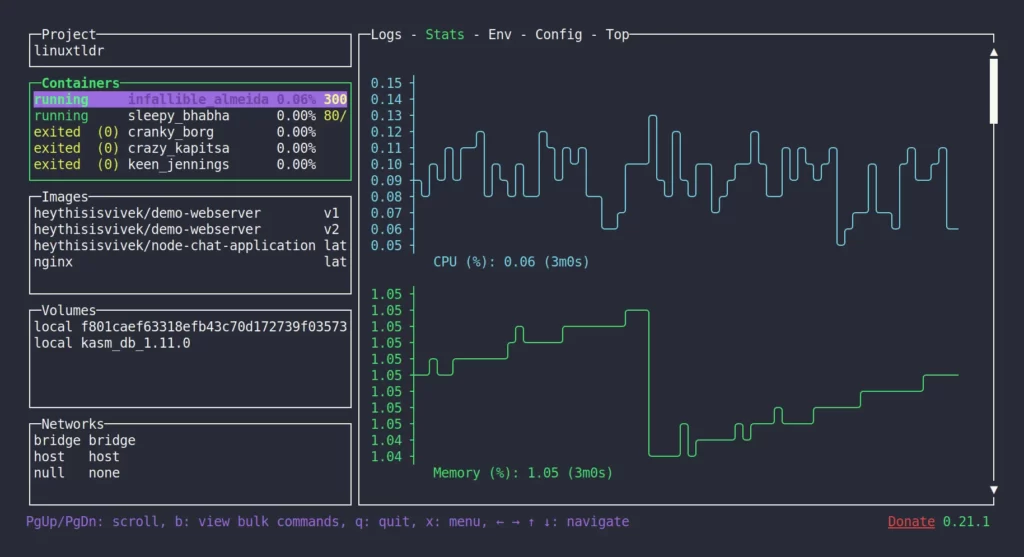
\includegraphics[width=.9\linewidth]{imgs/LazyDocker.png}
    \caption{LazyDocker main screen}
    \label{fig:enter-label}
\end{figure}

\textbf{Dolphie}: A utility for SQL database analytics

\begin{figure}[htbp]
    \centering
    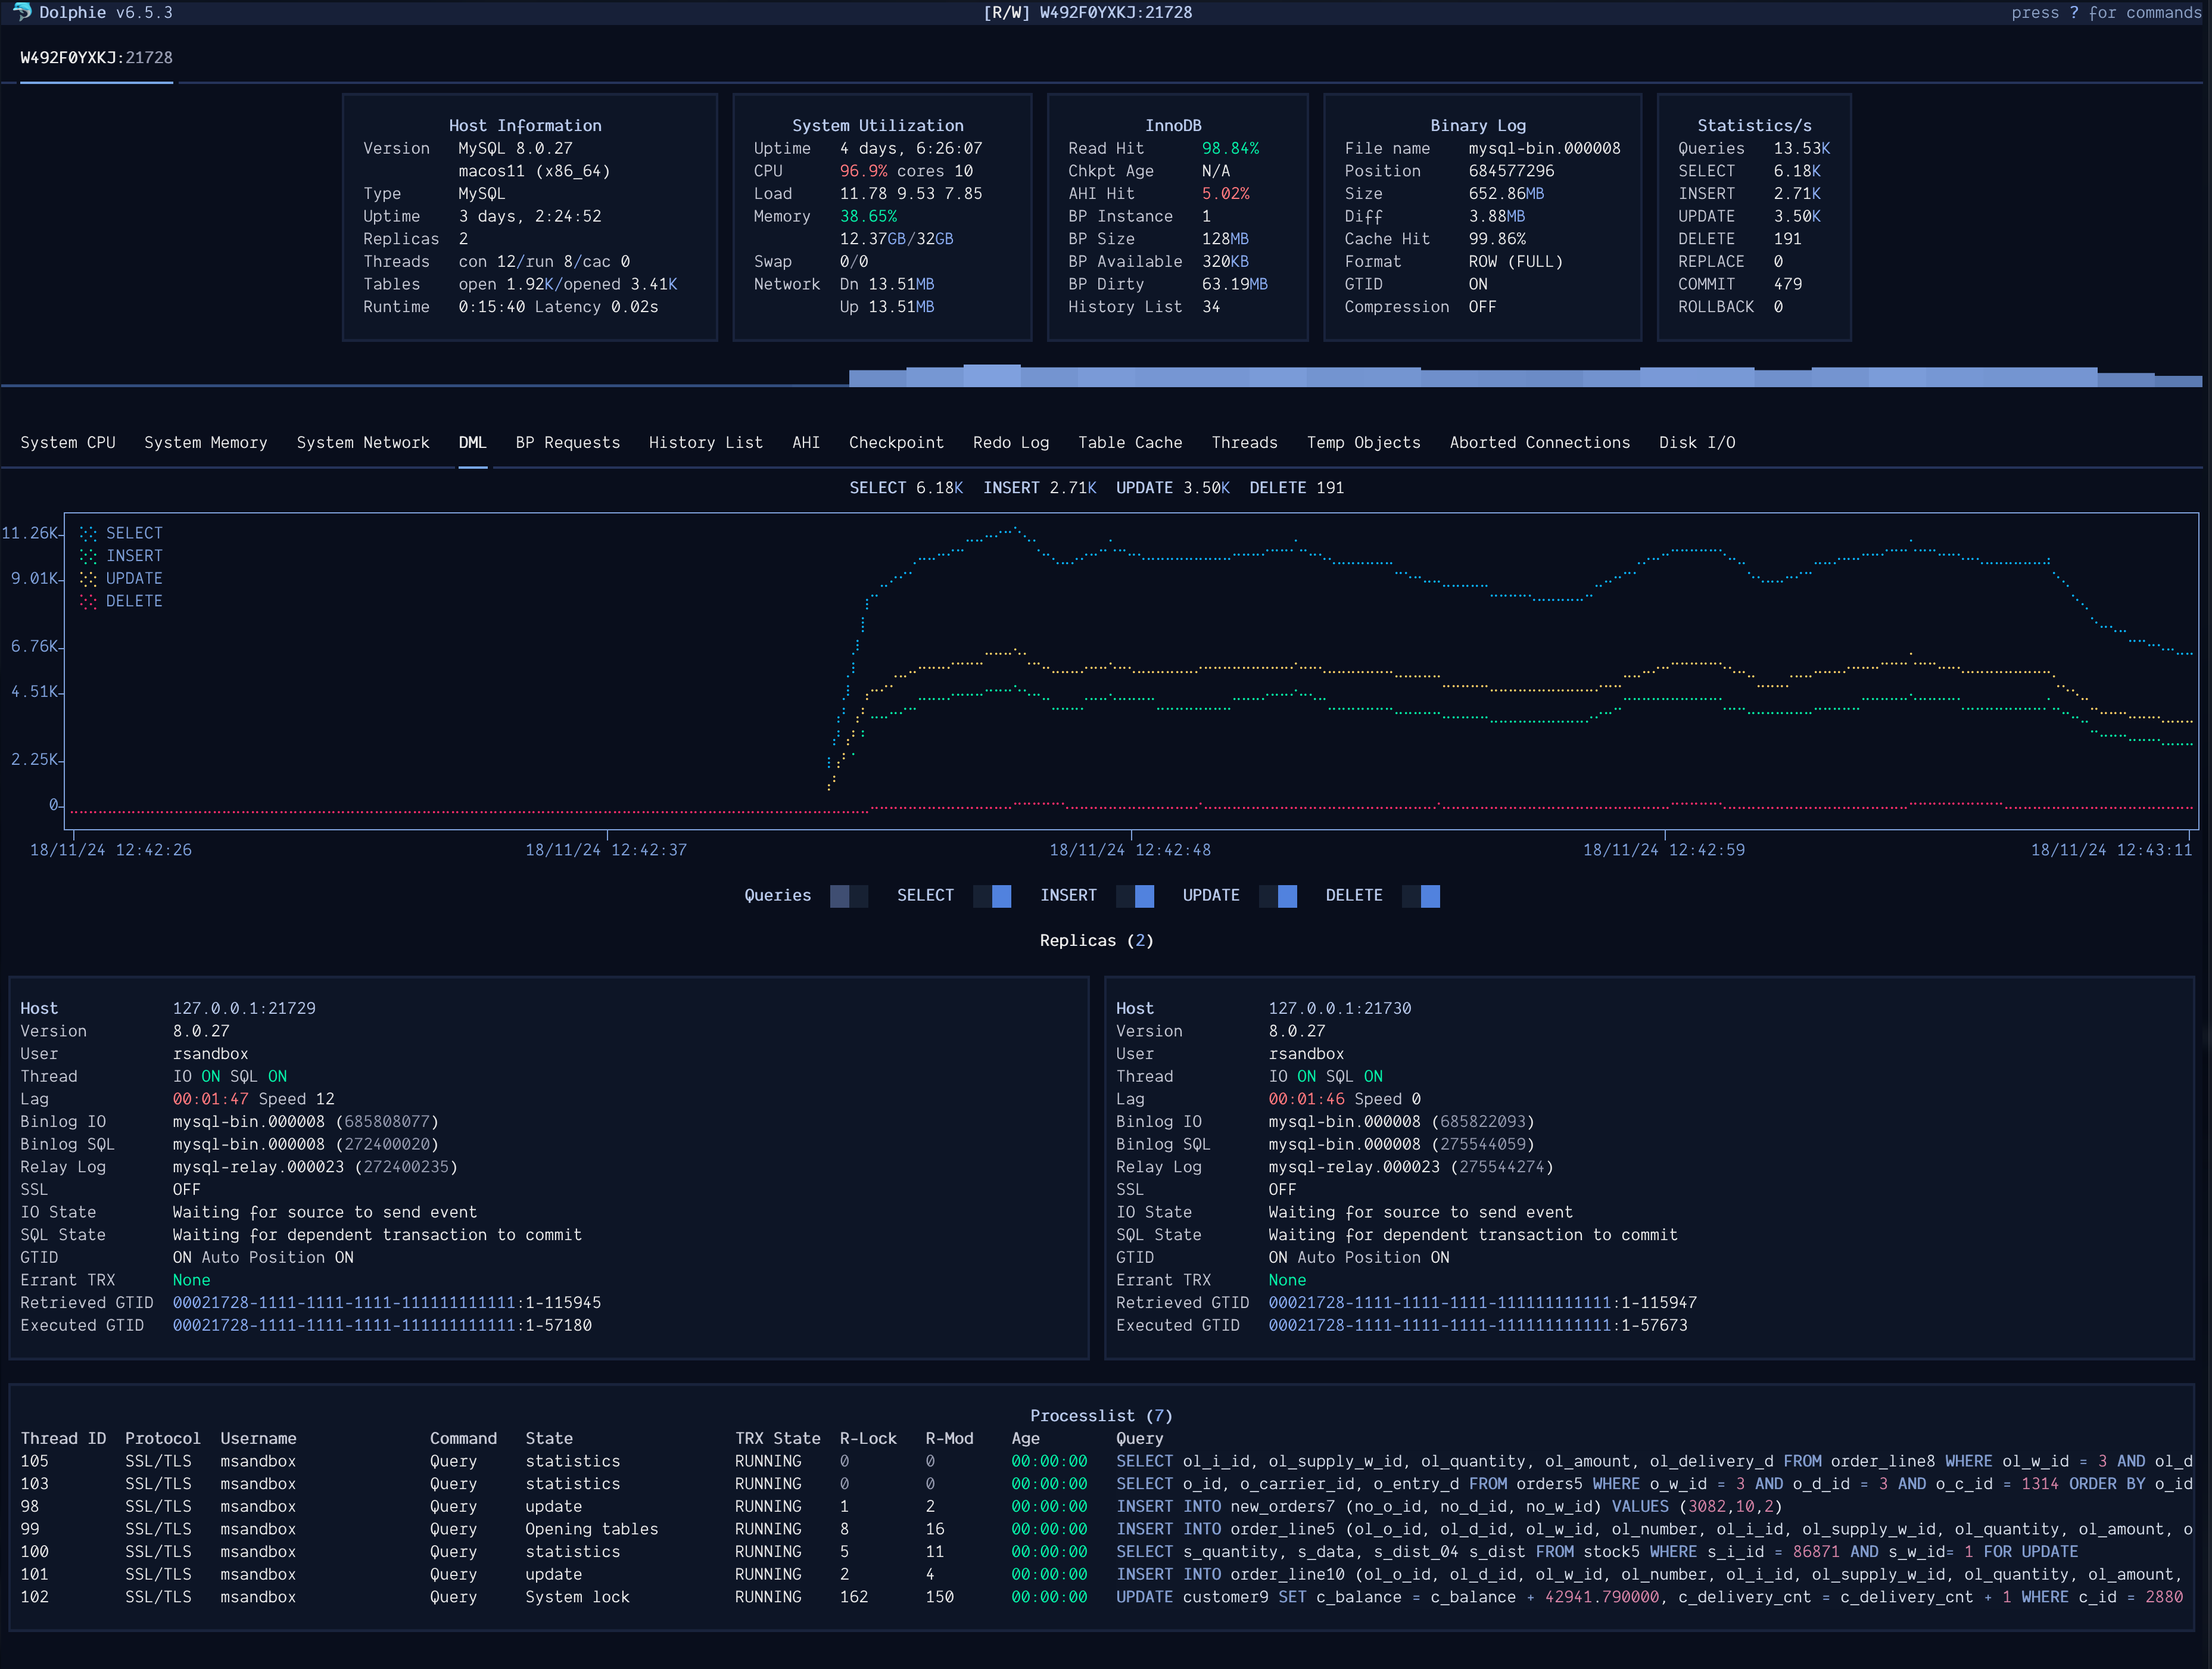
\includegraphics[width=.7\linewidth]{imgs/Dolphie.png}
    \caption{Dolphie main screen}
    \label{fig:enter-label}
\end{figure}

These are tools I personally use daily and find convenient. They allow me to quickly access necessary information. 

\subsection{LazyDocker Analysis}\label{subsec:ld_analysis}

To understand how exactly these tooks work, I analyzed LazyDocker.

\begin{figure}[htbp]
    \centering
    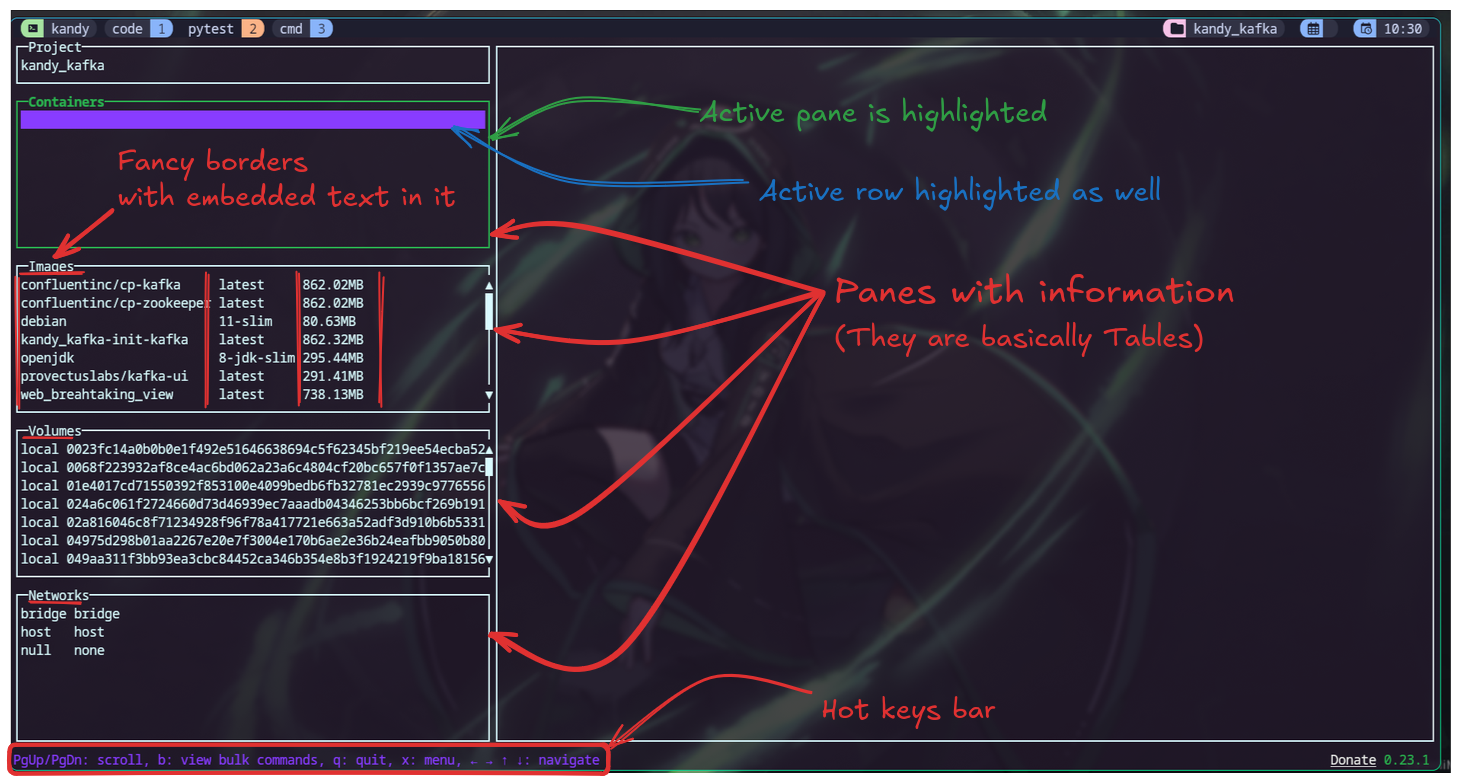
\includegraphics[width=.9\linewidth]{imgs/LazyDockerAnalysis.png}
    \caption{Lazydocker main screen analysis}
    \label{fig:lazydocker_analysis}
\end{figure}

When launching the utility, we can see the compact and minimalist design. All necessary categories are divided into panes, and navigation between them is performed by pressing \texttt{Tab}/\texttt{Shift+Tab} or using arrow keys. At the bottom of the screen, there’s also a bar with shortcut keys.

Panes are the most critical component of this interface. They display information, and their layout heavily influences the user experience. In the case of LazyDocker, the panes work as tables or lists of options. Beyond names, they show essential information, allowing users to navigate without guessing and compare container performance without opening detailed logs.

Additionally, there’s one large pane with detailed information about the selected container/image or network. This pane occupies more than half the screen, providing ample space for detailed data.

\begin{figure}[htbp]
    \centering
    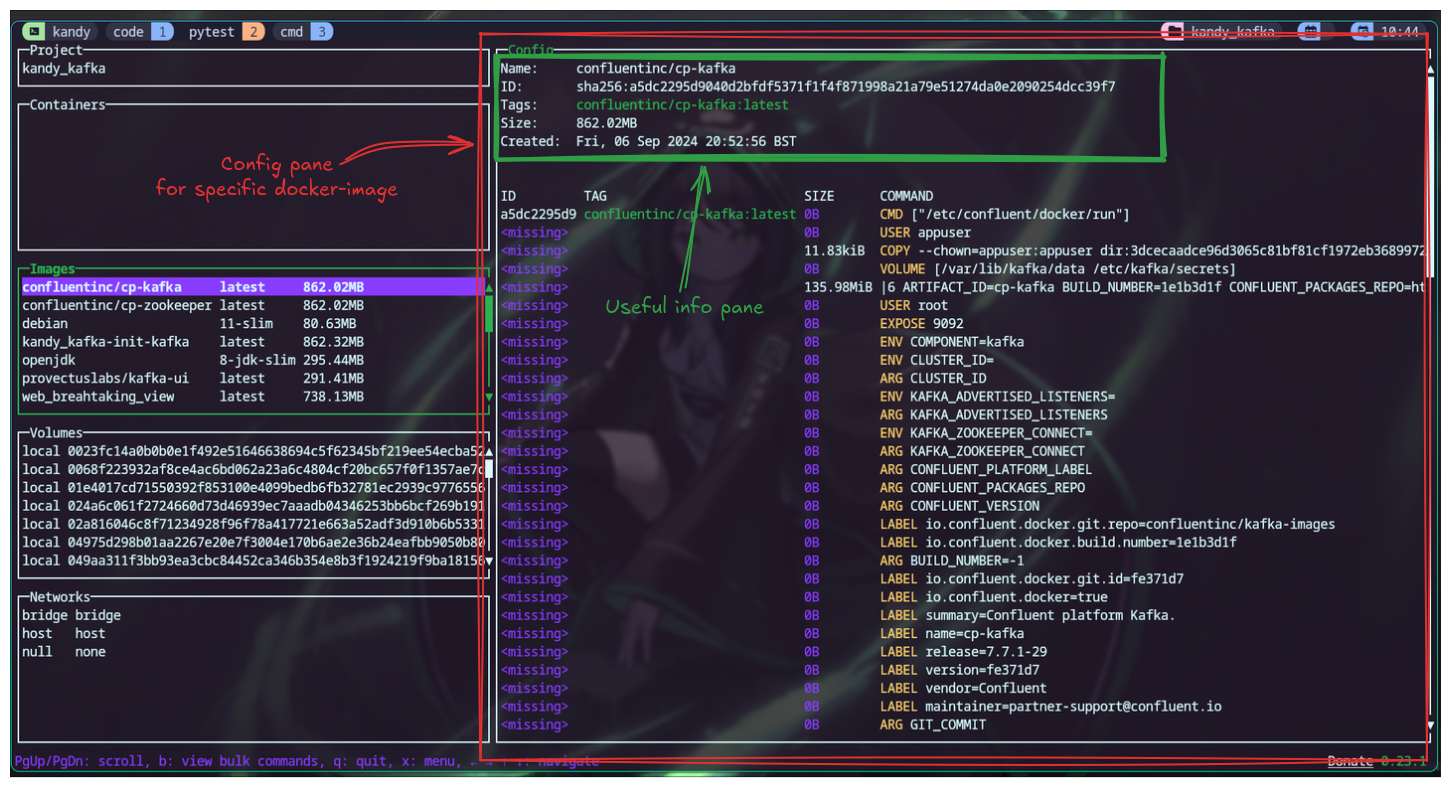
\includegraphics[width=.9\linewidth]{imgs/LazyDockerConfigPane.png}
    \caption{LazyDocker: Config pane}
    \label{fig:ld_big_pane}
\end{figure}


This pane is divided into several tabs. Besides configuration tab (\ref{fig:ld_big_pane}), you can view statistics for each container (\ref{fig:ld_stats_screen}), environment variables (\ref{fig:ld_env_pane}), and resource usage (\ref{fig:ld_top_pane}). This pane is the primary and most convenient feature for day-to-day Docker management. I believe a similar approach could be applied to my product.

\begin{figure}[htbp]
\centering
\begin{subfigure}{.5\textwidth}
    \centering
    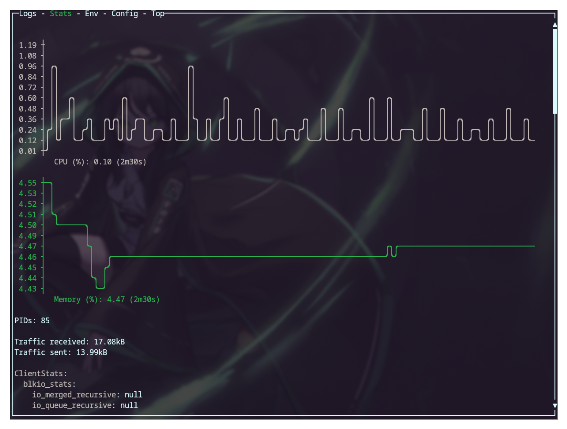
\includegraphics[width=.8\linewidth]{imgs/LazyDockerStatsPane.png}
    \caption{Stats}
    \label{fig:ld_stats_screen}
\end{subfigure}%
\begin{subfigure}{.5\textwidth}
    \centering
    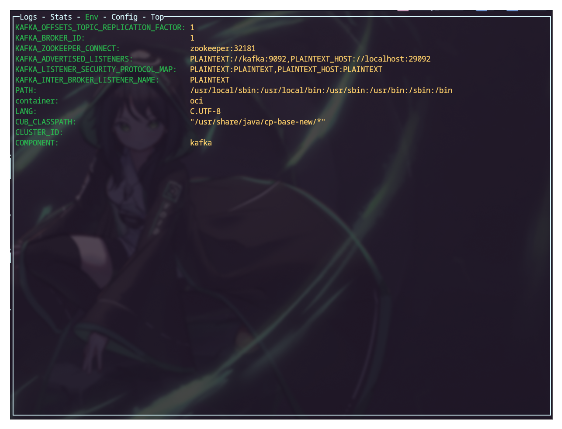
\includegraphics[width=.8\linewidth]{imgs/LazyDockerEnv.png}
    \caption{Env}
    \label{fig:ld_env_pane}
\end{subfigure}

\begin{subfigure}{.5\textwidth}
    \centering
    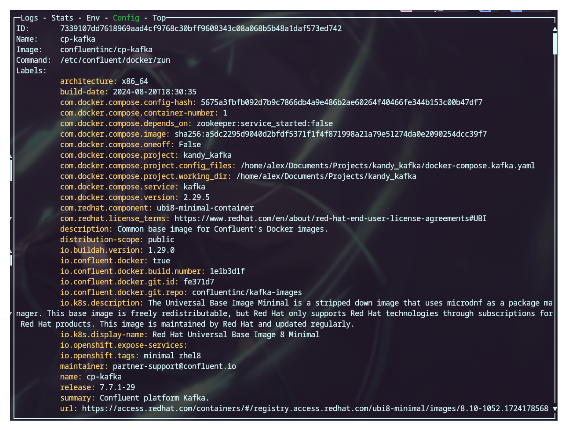
\includegraphics[width=.8\linewidth]{imgs/LazyDockerConfig.png}
    \caption{Config}
    \label{fig:ld_config_pane}
\end{subfigure}%
\begin{subfigure}{.5\textwidth}
    \centering
    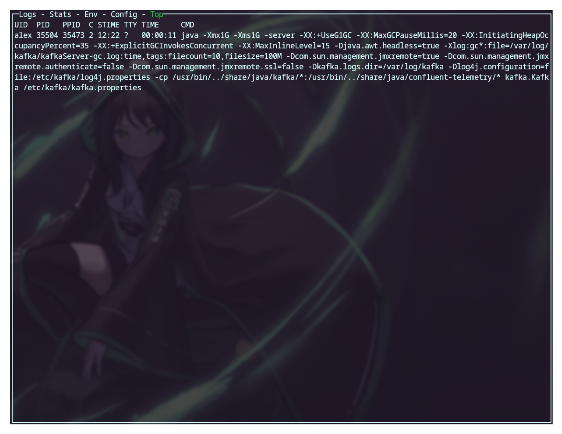
\includegraphics[width=.8\linewidth]{imgs/LazyDockerTopPane.png}
    \caption{Top}
    \label{fig:ld_top_pane}
\end{subfigure}
\caption{Big pane tabs}
\end{figure}

\begin{figure}[htbp]
    \centering
    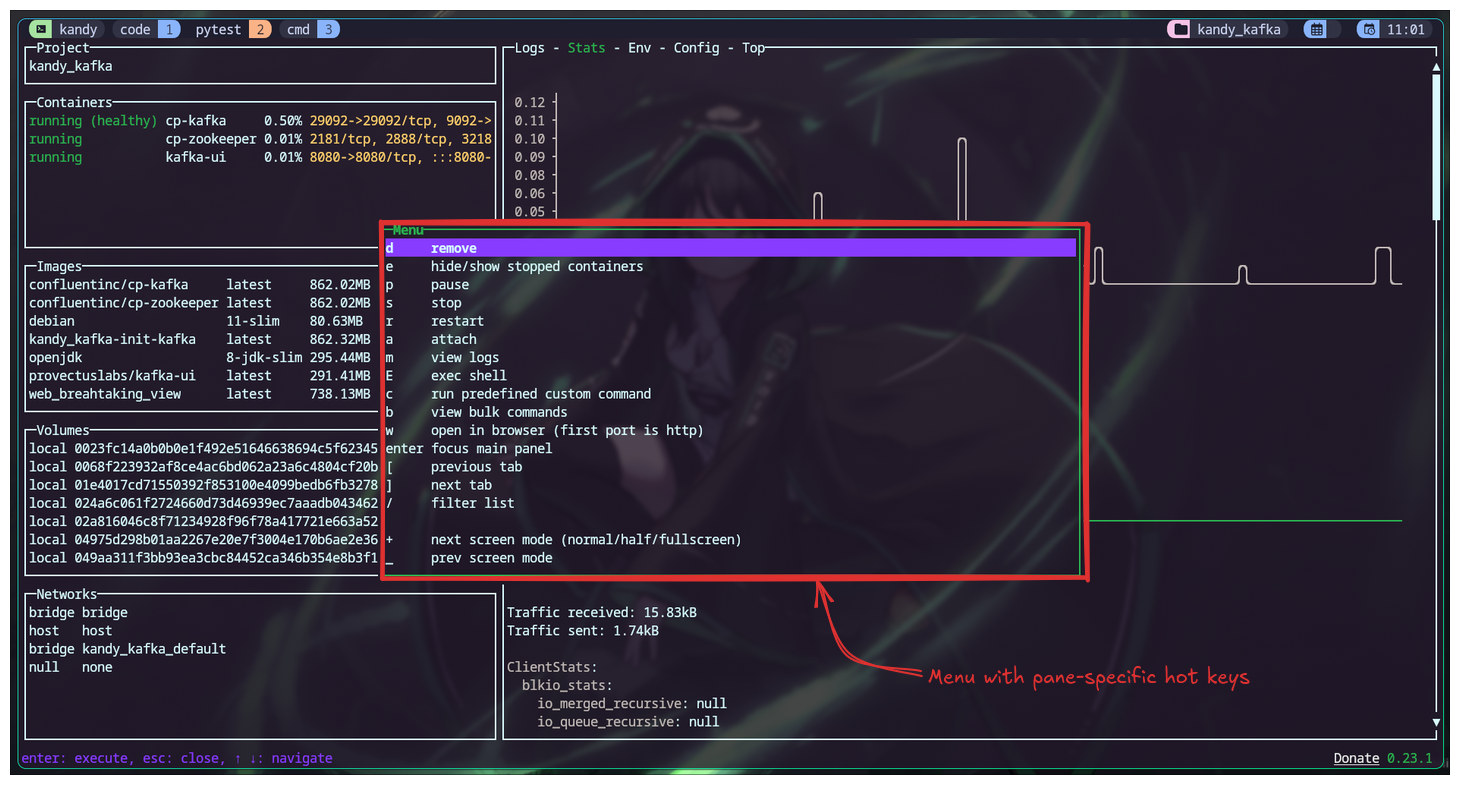
\includegraphics[width=.9\linewidth]{imgs/LazyDockerHotKeysMenu.png}
    \caption{Hotkey Menu}
    \label{fig:enter-label}
\end{figure}

Lastly, pressing a hotkey \texttt{X} opens a menu with a wide range of commands. Hotkeys are designed to speed up processes, and this kind of menu, which consolidates all necessary commands, significantly enhances efficiency. Unlike the bar, this menu allows for a detailed description of each key binding.

This is probably my favorite feature of LazyDocker because it eliminates the need to exit the utility and type lengthy commands to accomplish simple tasks and basiclly speeds up my work several times. I definitely plan to implement such a menu in my product.


\subsection{Conclusions}

After analyzing LazyDocker, I identified key features that could be useful in creating my own utility:

\begin{itemize}
    \item \textbf{Pane-based layout}: This structure looks harmonious and logical for such utilities. Each pane functions as a container, simplifying the logic of information display.
    \item \textbf{Table-like panes}: Displaying data in this format aligns with Kafka’s structure and is likely the optimal solution.
    \item \textbf{Menu and hotkey bar}: These elements make navigation through the interface a quick and effortless task, often requiring no conscious thought.
    \item \textbf{Tabbed panes}: As with the large pane, using tabs instead of separate screens can sometimes be more convenient and logical.
    \item \textbf{Colors}: Though not explicitly mentioned earlier, colors play a vital role both aesthetically and functionally. Highlighting the active pane, using a “traffic light” system to display container statuses, and syntax highlighting for configurations all enhance the user experience.
\end{itemize}

By incorporating these features, I aim to develop a TUI application that is both efficient and user-friendly.

\newpage
\section{Features of the proposed solution}
\label{sec:proposed_features}
\begin{figure}[htbp]
    \centering
    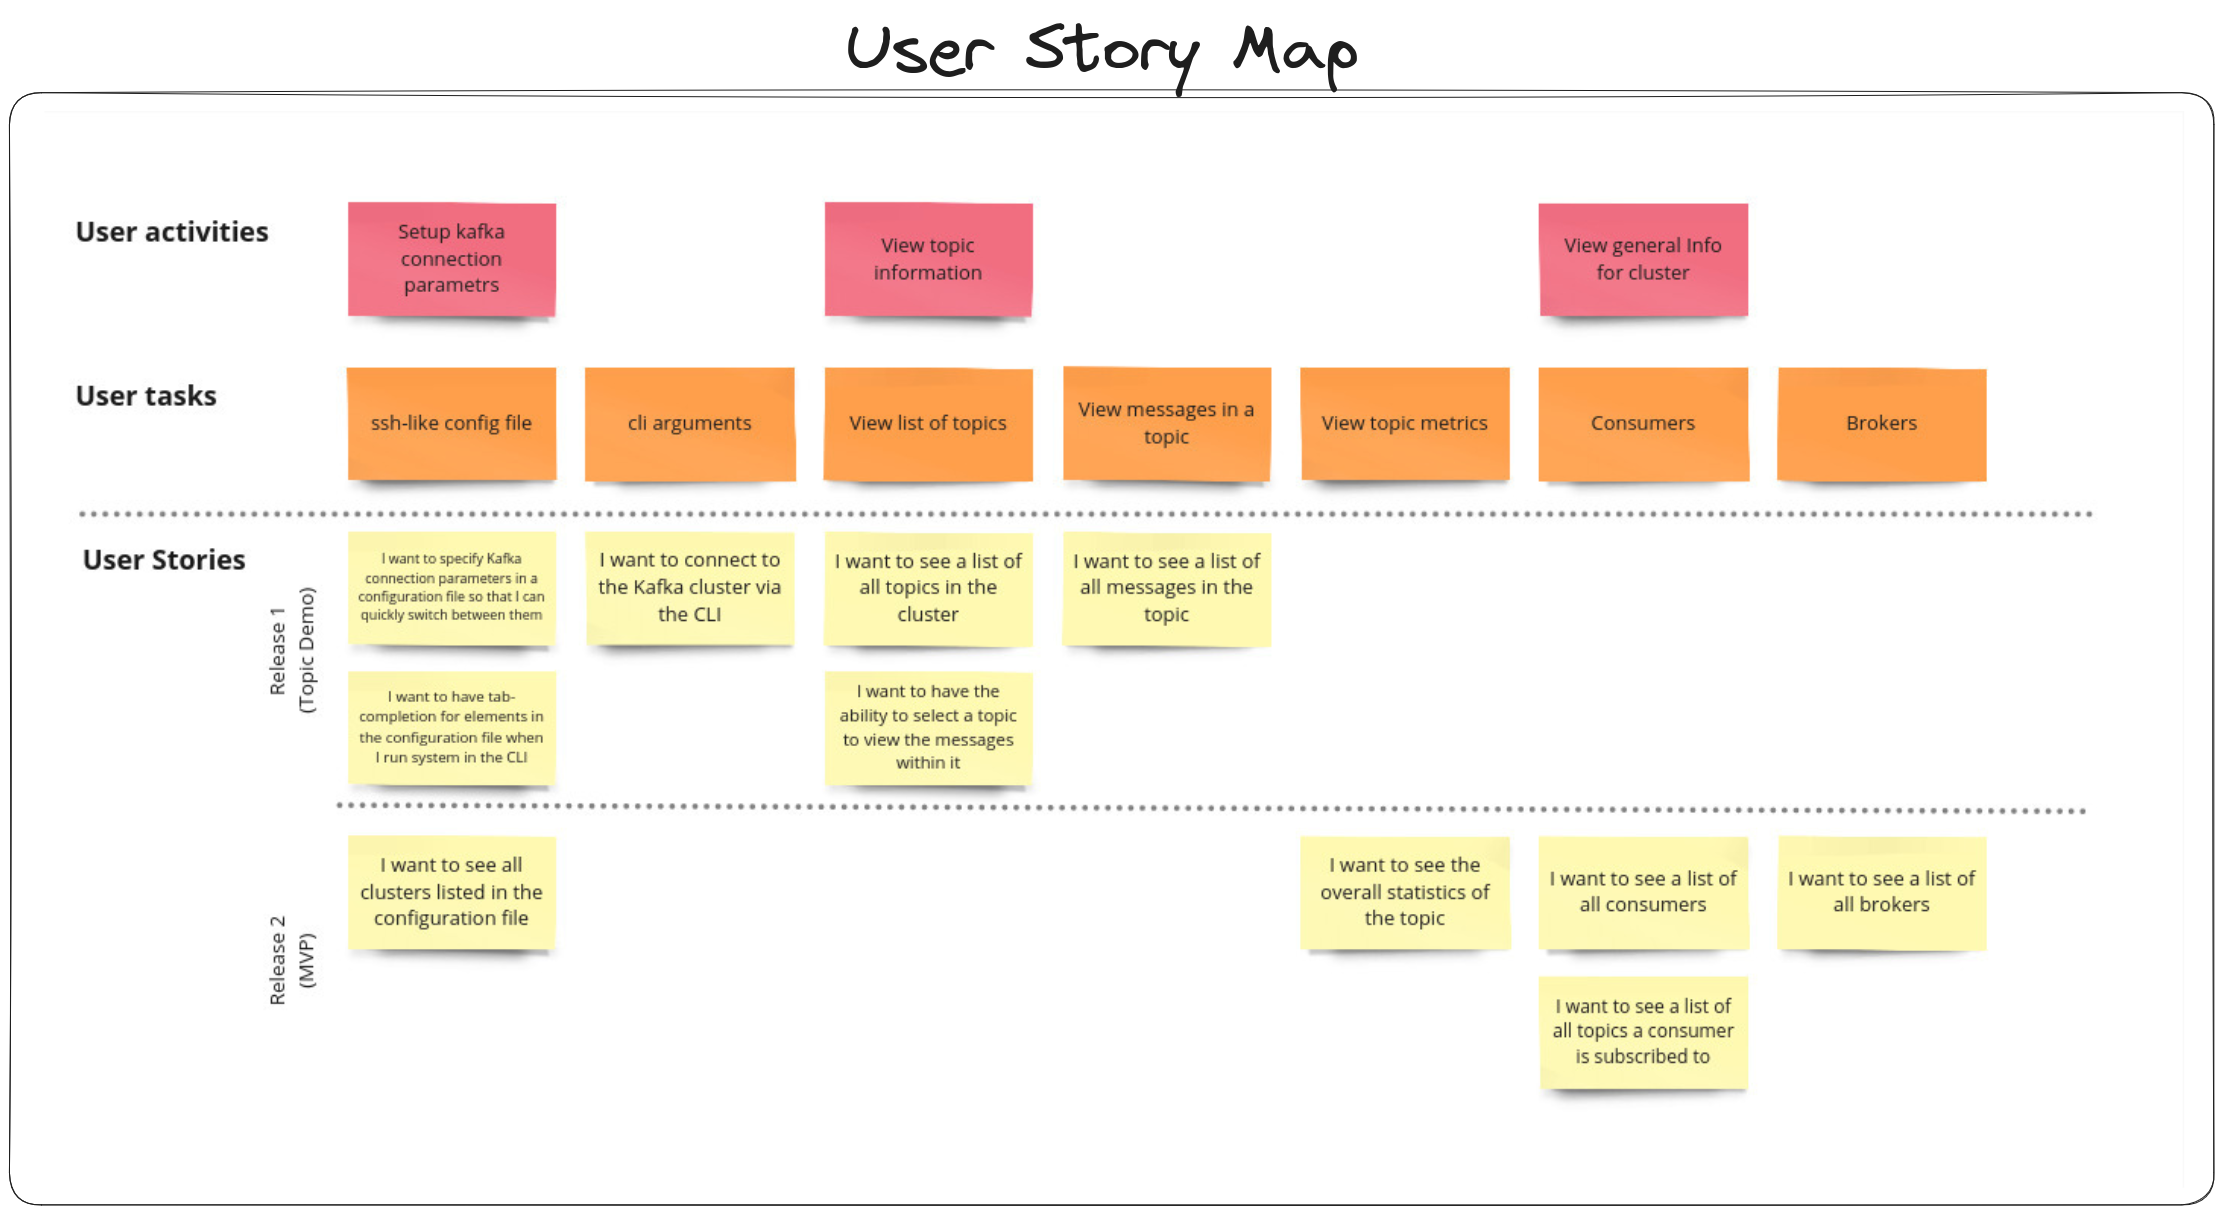
\includegraphics[width=1\linewidth]{imgs/UserStoryMap.png}
    \label{fig:USM}
\end{figure}

To outline the initial application concept and plan for future development, I chose to use User Story Mapping (USM). This approach provides a user-centered perspective, aiding in prioritizing features across different development phases. USM is an agile approach to requirements engineering, composed of several key elements:

\begin{enumerate} \item \textbf{User Activity:} This step involves identifying the main activities users will perform within the system, representing the core actions they take to achieve their goals. \item \textbf{User Tasks:} Within each user activity, specific tasks are defined. These tasks represent the necessary steps users must follow to accomplish the activity. \item \textbf{User Stories:} Each task is further refined into user stories. These stories represent the functionalities or features needed to fulfill the task from the user's perspective. \end{enumerate}

In a User Story Map, user stories are organized into swimlanes based on their release phases. Releases indicate the prioritization of user stories, outlining which ones should be completed first. The essential structure of USM lies in its sequential arrangement of user tasks from left to right, aiming to provide a comprehensive overview of user interactions with the system. This format helps ensure a clear understanding of user needs and workflows.

One of the main advantages of USM over other requirements engineering techniques is its flexibility to accommodate changes based on user feedback. Its visual representation also aids in understanding the system from the user’s perspective, enhancing communication and collaboration among stakeholders.

On the map, tasks are divided into two releases: Topic Demo and MVP. The Topic Demo represents the initial stage, where I will create the application framework, TUI, and add the essential topic-viewing feature. This demo serves as a basis for consulting with my stakeholder and allows for adjustments to the USM if needed.

After consulting with Sarah, I will refine the application according to her feedback and proceed to work on the second release, MVP (Minimal Viable Product). This release will include additional features, such as displaying statistics across all topics and enabling interaction with consumer groups.

\section{Limitations of my solution:}

The primary limitation of this solution is time. As this project is part of the A-level coursework, alongside other assignments, my task estimates may be overly optimistic. Working independently, I may realistically only be able to implement a portion of the planned functionality.

Additionally, there are limitations associated with the libraries I intend to use. Currently, I am considering urwid or textual for developing the TUI (Text User Interface). However, urwid, for instance, does not support a broad range of terminal types and may perform inconsistently in certain environments, which could pose challenges and restrict my solution’s effectiveness.

\chapter{Requirements}

\section{Software product quality model}

\begin{figure}[htbp]
    \centering
    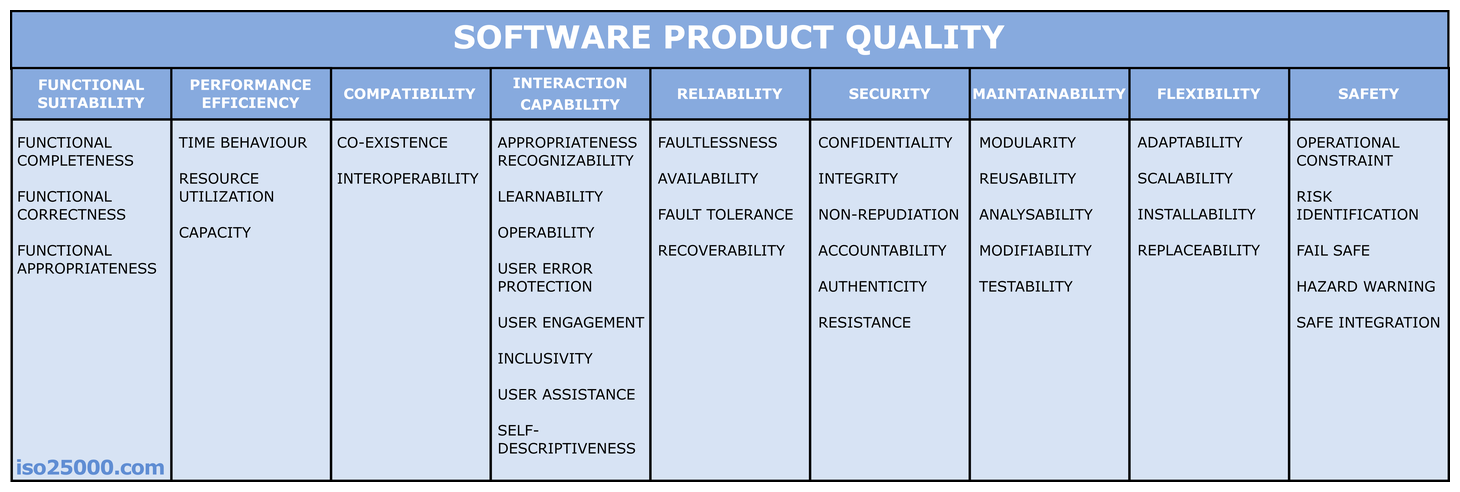
\includegraphics[width=1\linewidth]{imgs/ISO25010.png}
    \label{fig:quality_model}
\end{figure}

    I based my quality requirements on the ISO 25010 standard, which outlines the key characteristics of any software product, and developed a quality model using the QAS (Quality Attribute Scenarios) methodology. To achieve this, I identified critical attributes by referencing both interviews with Sarah and industry standards. A description of the model and its attributes is provided below.
    
\newpage

\subsection{Quality Attribute Scenarios (QAS)}

Each quality attribute is defined through quality attribute scen-arios, which must adhere to the six-part rule. For more information on this method, see https://wstomv.win.tue.nl/edu/2ii45/year-0910/Software\_Architecture\_in\_Practice\_2nd\_Edition\_Chapter4.pdf

\begin{table}[h!]
    \centering
    \renewcommand{\arraystretch}{1.3} % Set a comfortable line spacing
    \begin{adjustbox}{max width=\textwidth} % Fit table to page width
        \begin{tabular}{| p{3.5cm} | p{10.5cm} |}
            \hline
            \textbf{Term} & \textbf{Description} \\ \hline
            Stimulus & Describes an event arriving at the system, like a performance event, user operation, or security attack. A stimulus for modifiability could be a modification request, while for testability, it could be a phase completion. \\ \hline
            Stimulus Source & The origin of a stimulus, affecting how the system treats it. For example, a trusted user’s request may be handled differently from an untrusted user's. \\ \hline
            Response & Specifies how the system or developers should act in response to the stimulus, detailing responsibilities at runtime or during development. \\ \hline
            Response Measure & Defines how to judge if the response meets requirements, helping determine if the system or developer actions are sufficient. \\ \hline
            Environment & The context in which the scenario occurs, which qualifies the stimulus and influences system response. \\ \hline
            Artefact & The part of the system to which the requirement applies, often the entire system but sometimes only specific components. \\ \hline
        \end{tabular}
    \end{adjustbox}
    \caption{Definitions of Key Terms}
\end{table}

\subsection{Environment}
    I am gonna use my laptop as a \textbf{normal operating conditions} for several reasons. First of all, it's always at hand, so I don't need to worry about logistics or where I'll be testing the product. Secondly, I have a fairly average laptop in terms of specifications, so if the utility works smoothly on it, it will likely work on more powerful machines as well. Therefore, all hardware requirements are based on the basic characteristics of my device and all software requirements are based on the installed software on the my machine.

\begin{table}[h!tbp]
\centering
\begin{tabular}{| l | l |}
\hline
\textbf{Part of environment} & \textbf{Variable} \\
\hline
OS & Manjaro Linux 23.1.4 (Vulcan) \\
\hline
Terminal Emulator & Kitty 0.31.0 \\
\hline
Kafka version & confluentinc/cp-kafka:7.7.1\\
\hline
Python version & 3.11.4 \\
\hline
CPU & 1.60 GHz \\
\hline
RAM & 4 GB \\
\hline
Docker version & 25.0.3 \\
\hline
Python libs versions & Specified in the file \textbf{pyproject.toml} in~Appendix:\ref{appendix:libs} \\
\hline

\end{tabular}

\end{table}
As Kafka will be deployed on the same system where Kandy is tested, I anticipate virtually negligible latency when it comes to communicating between services

\newpage
\subsection{Scenarios}
\begin{small}
\begin{table}[h!tbp]
\centering
\renewcommand{\arraystretch}{1.3} % Adjust row spacing for readability
\begin{tabular}{|l|p{9cm}|}
\hline
\textbf{Relevant Quality Attributes} & Performance Efficiency, Reliability \\ \hline
\textbf{Stimulus} & A user selects a Kafka topic and requests to fetch messages. \\ \hline
\textbf{Source} & User interacting with the UI. \\ \hline
\textbf{Environment} & Kafka cluster is online and accessible; the system is running under normal conditions. \\ \hline
\textbf{Artefact} & System \\ \hline
\textbf{Response} & The system retrieves and displays the 50 most recent messages from the selected topic while ensuring the UI remains operational. \\ \hline
\textbf{Response Measure} & Messages are displayed within 10 seconds of the request, and the UI remains responsive. \\ \hline
\textbf{Possible Issues} & High latency in Kafka communication might delay message retrieval. UI freezing if asynchronous fetching is not properly implemented. \\ \hline
\textbf{Justification} & A response time of 10 seconds aligns with the industry standard for maintaining user focus. Research from the Nielsen Norman Group (\url{https://www.nngroup.com/articles/response-times-3-important-limits/}) shows that users lose focus when waiting for over 10 seconds, leading to a degraded experience. This boundary ensures usability while accounting for network and processing delays. \\ \hline
\end{tabular}
\caption{Scenario: Fetching Messages from Kafka Topics}
\end{table}

\begin{table}[h!tbp]
\centering
\renewcommand{\arraystretch}{1.3} % Adjust row spacing for readability
\begin{tabular}{|l|p{9cm}|}
\hline
\textbf{Relevant Quality Attributes} & Usability, Performance Efficiency \\ \hline
\textbf{Stimulus} & A user inputs a search query to filter Kafka topics. \\ \hline
\textbf{Source} & User interacting with the UI. \\ \hline
\textbf{Environment} & The system is running under normal conditions with topics preloaded from Kafka. \\ \hline
\textbf{Artefact} & UI \\ \hline
\textbf{Response} & The system applies the query to filter the list of topics dynamically, displaying matching results in real-time. \\ \hline
\textbf{Response Measure} & Filtered topics are displayed within 1 second of query input. \\ \hline
\textbf{Possible Issues} & Large topic lists might delay filtering. Regex implementation could fail for malformed queries. Poor responsiveness may degrade user experience. \\ \hline
\textbf{Justification} & A 1-second response for search results is supported by Jakob Nielsen's response-time limits (\url{https://www.nngroup.com/articles/response-times-3-important-limits/}), which highlight that users feel the system operates instantaneously at this threshold. \\ \hline
\end{tabular}
\caption{Scenario: Searching for Kafka Topics}
\end{table}

\begin{table}[h!tbp]
\centering
\renewcommand{\arraystretch}{1.3} % Adjust row spacing for readability
\begin{tabular}{|l|p{9cm}|}
\hline
\textbf{Relevant Quality Attributes} & Reliability, Fault Tolerance \\ \hline
\textbf{Stimulus} & Kafka becomes unavailable or unreachable. \\ \hline
\textbf{Source} & Kafka infrastructure failure. \\ \hline
\textbf{Environment} & Kafka is down or the connection details are misconfigured. \\ \hline
\textbf{Artefact} & System \\ \hline
\textbf{Response} & The system notifies the user of the error and terminates gracefully, ensuring that no processes hang or crash. \\ \hline
\textbf{Response Measure} & The error message is displayed within 1 second, and the system remains stable. \\ \hline
\textbf{Possible Issues} & The system could hang during reconnect attempts. Vague error messages might confuse users. Exit mechanisms may not properly clean up resources. \\ \hline
\textbf{Justification} & A 1-second boundary for error feedback ensures users are informed promptly without unnecessary delay, aligning with ISO 25010’s emphasis on fault tolerance. Immediate user feedback helps in scenarios where long-running processes could otherwise cause confusion. \\ \hline
\end{tabular}
\caption{Scenario: Handling Kafka Connection Errors}
\end{table}

\begin{table}[h!tbp]
\centering
\renewcommand{\arraystretch}{1.3} % Adjust row spacing for readability
\begin{tabular}{|l|p{9cm}|}
\hline
\textbf{Relevant Quality Attributes} & Modifiability, Usability \\ \hline
\textbf{Stimulus} & A user initializes the application with host and port details provided through CLI flags. \\ \hline
\textbf{Source} & User invoking the system from the command line. \\ \hline
\textbf{Environment} & CLI arguments are passed at runtime; no configuration file is provided. \\ \hline
\textbf{Artefact} & System \\ \hline
\textbf{Response} & The system validates the arguments and establishes a connection to Kafka using the specified host and port. \\ \hline
\textbf{Response Measure} & The connection is established successfully, and invalid arguments are rejected with clear error messages within 1 second. \\ \hline
\textbf{Possible Issues} & Users might provide incomplete or conflicting arguments. Validation logic might miss invalid inputs. \\ \hline
\textbf{Justification} & A response time of 1 second for invalid argument rejection aligns with usability principles (ISO 9241) and ensures smooth configuration. Immediate feedback minimizes user frustration and supports modifiability in diverse environments. \\ \hline
\end{tabular}
\caption{Scenario: Configuring Kafka Connection via CLI}
\end{table}

\begin{table}[h!tbp]
\centering
\renewcommand{\arraystretch}{1.3} % Adjust row spacing for readability
\begin{tabular}{|l|p{9cm}|}
\hline
\textbf{Relevant Quality Attributes} & Functional Suitability, Performance Efficiency \\ \hline
\textbf{Stimulus} & A user selects a topic to view its metadata. \\ \hline
\textbf{Source} & User interacting with the UI. \\ \hline
\textbf{Environment} & Kafka cluster is online and the system is running under normal conditions. \\ \hline
\textbf{Artefact} & System \\ \hline
\textbf{Response} & The system retrieves and displays the topic’s metadata, including partition count and message offset details. \\ \hline
\textbf{Response Measure} & Metadata is displayed within 2 seconds of selection. \\ \hline
\textbf{Possible Issues} & Large numbers of topics might delay metadata retrieval. Poor UI design could result in unclear metadata presentation. \\ \hline
\textbf{Justification} & A 2-second response time ensures an acceptable balance between data retrieval and user experience, as supported by ISO 25010 for functional suitability and response times for non-critical data. \\ \hline
\end{tabular}
\caption{Scenario: Displaying Topic Metadata}
\end{table}

\begin{table}[h!tbp]
\centering
\renewcommand{\arraystretch}{1.3} % Adjust row spacing for readability
\begin{tabular}{|l|p{9cm}|}
\hline
\textbf{Relevant Quality Attributes} & Usability, Reliability \\ \hline
\textbf{Stimulus} & A user provides invalid input in a search field or configuration form. \\ \hline
\textbf{Source} & User interacting with the UI. \\ \hline
\textbf{Environment} & The system is running under normal conditions. \\ \hline
\textbf{Artefact} & System \\ \hline
\textbf{Response} & The system validates the input, rejects invalid entries, and notifies the user with a descriptive error message. \\ \hline
\textbf{Response Measure} & Input validation occurs within 1 second, and error messages are displayed immediately. \\ \hline
\textbf{Possible Issues} & Poor error messages might confuse users. Invalid inputs might bypass validation logic. \\ \hline
\textbf{Justification} & Immediate validation aligns with industry practices for reliability and ISO 25010 usability principles. Error feedback ensures clarity and prevents incorrect system states. \\ \hline
\end{tabular}
\caption{Scenario: Invalid User Input in UI}
\end{table}


\begin{table}[h!tbp]
\centering
\renewcommand{\arraystretch}{1.3} % Adjust row spacing for readability
\begin{tabular}{|l|p{9cm}|}
\hline
\textbf{Relevant Quality Attributes} & Testability, Maintainability \\ \hline
\textbf{Stimulus} & A developer modifies code and runs the test suite. \\ \hline
\textbf{Source} & Developer using the testing framework. \\ \hline
\textbf{Environment} & The system is in active development or integrated with CI/CD pipelines. \\ \hline
\textbf{Artefact} & System \\ \hline
\textbf{Response} & Tests validate critical paths and edge cases. \\ \hline
\textbf{Response Measure} & At least 90\% code coverage with no major untested areas. \\ \hline
\textbf{Possible Issues} & Poor test coverage could miss critical issues. Complex code paths may lead to gaps in edge case testing. \\ \hline
\textbf{Justification} & High test coverage ensures confidence in the codebase and reduces regressions. \\ \hline
\end{tabular}
\caption{Scenario: Comprehensive Test Coverage}
\end{table}

\end{small}

\newpage
\section{Success criteria}

\begin{table}[h!tbp]
\centering
\renewcommand{\arraystretch}{1.3} % Adjust row spacing for readability
\begin{adjustbox}{max width=\textwidth}
\begin{tabular}{|p{3.5cm}|p{6.5cm}|p{4.5cm}|p{4cm}|}
\hline
\textbf{Criterion} & \textbf{Success Measure} & \textbf{Evidence} & \textbf{Justification} \\ \hline

\textbf{Connecting to Kafka} & 
The system successfully connects to the Kafka cluster using provided host and port details. Invalid configurations are rejected with a descriptive error message displayed within 1 second. & 
Connection logs showing successful connections with valid inputs and immediate rejection of invalid configurations & 
Connecting to Kafka is foundational for all other functionality, ensuring the system can access topics and messages. Immediate error feedback prevents wasted time debugging. \\ \hline

\textbf{Fetching Topics} & 
The system retrieves the list of Kafka topics from the cluster and displays them in the UI within 10 seconds of the request. & 
System logs confirming topics fetched in under 10 seconds. & 
Fetching topics is critical for enabling user interaction with Kafka data. The 10-second limit aligns with industry standards for maintaining user focus. \\ \hline

\textbf{Fetching Messages} & 
The system retrieves the 50 the most recent messages from a selected Kafka topic asynchronously. Messages are displayed within 10 seconds, and the UI remains operational during this process. & 
Execution logs confirming message retrieval time. Manual testing reports confirming UI responsiveness during retrieval & 
Message fetching is a core requirement for Kafka consumers. The 10-second limit ensures a responsive user experience, even for large topics. \\ \hline

\textbf{Sorting Topics} & 
The user can apply sorting criteria (e.g., by size or partition count) to the displayed list of topics. Sorted results are updated in the UI within 2 seconds of the user request. & 
Performance benchmarks showing sorting operations completed within 2 seconds. Functional tests verifying sorting behavior & 
Sorting improves usability by allowing users to organize and locate topics efficiently. The 2-second limit ensures the UI remains responsive and intuitive. \\ \hline

\textbf{Input Validation} & 
All user inputs, such as CLI flags or search queries, are validated. Invalid inputs trigger immediate rejection and display a descriptive error message within 1 second. & 
Validation logs showing immediate error feedback. Unit test results confirming coverage for all input validation scenarios & 
Validating user input ensures the system remains robust and prevents errors caused by invalid configurations or queries. Immediate feedback aligns with usability best practices. \\ \hline

\textbf{UI Responsiveness} & 
The system UI remains fully operational and responsive during Kafka interactions, including fetching topics, messages, and sorting operations. & 
Manual testing reports confirming no UI freezes during key interactions & 
A responsive UI is essential for maintaining a positive user experience. It ensures that interactions feel smooth, even when handling large datasets or performing complex operations. \\ \hline

\end{tabular}
\end{adjustbox}
\caption{Success Criteria for MVP}
\label{tab:success-criteria-mvp}
\end{table}


\chapter{Design}

Having identified the requirements and success criteria, I can now proceed with designing the system itself. The primary goal of this process is to create a structure that facilitates the addition of new features and the maintenance of the project while preserving or improving its functionality. A thoughtful design approach is essential to ensure effective system development, maintainability, scalability, and adaptability for future changes.

Any design process begins with the decomposition of the problem into manageable pieces of work and domain-specific elements. This activity often involves brainstorming.

As a visual thinker, I decided to create a diagram that depicts the elements and sections of the system being designed.

\section{Decomposition}

The first level of elements I identified is as follows:
\begin{itemize}
    \item Define core functional requirements
    \item Choose development technology
    \item Design user interface structure
    \item Test and debug
    \item Release and support
\end{itemize}

Since I am building a tool for an existing software system, my tool is heavily dependent on its core functionality and capabilities. Therefore, understanding and defining the core functional requirements is a high-priority activity.

Choosing suitable development technology is critical for several reasons. First, it must enable technical integration with Kafka. Second, I must have sufficient expertise in the chosen technology to ensure that the project is completed within the set timeline.

Given that the project goal is to create an application with a user interface (UI) to enhance how target users interact with Kafka, I need to carefully plan the UI's structure and design to ensure an optimal user experience.

Any software application requires an appropriate level of testing. To define what ``appropriate'' means for my application, I must consider how the system will be tested and determine the level of logging required to ensure that it works as expected.

The final phase of application development involves delivering the software to the target users. The process of installation and running the application is just as important as the application requirements themselves. Thus, I aim to plan ahead and identify the tools and strategies needed to make this process as seamless as possible.

In the following sections, I will explain my thought process for each element and how they contribute to the system's development.

\newpage

\subsection{Prioritization}
Features are categorized into \textbf{essential} (green), \textbf{desirable} (yellow), and \textbf{optional} (red):
\begin{figure}[htbp]
    \centering
    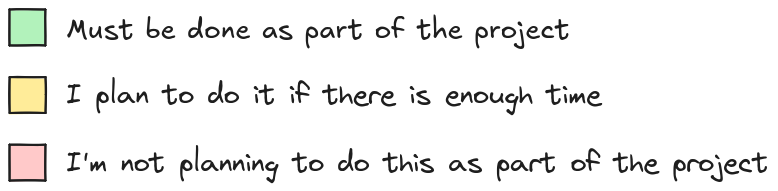
\includegraphics[width=.6\linewidth]{imgs/DesignLegend.png}
    \caption{System Design Diagram Legend}
    \label{fig:design_legend}
\end{figure}

For the full diagram, refer to \textbf{Appendix~\ref{appendix:system_design}}. Given the large size of the diagram, I will discuss its components and subdivisions separately in the following sections

\subsection{Core functional requirements}

As mentioned earlier, understanding and defining the core functional requirements is a high-priority activity. I have divided this into three main blocks:

\begin{figure}[htbp]
    \centering
    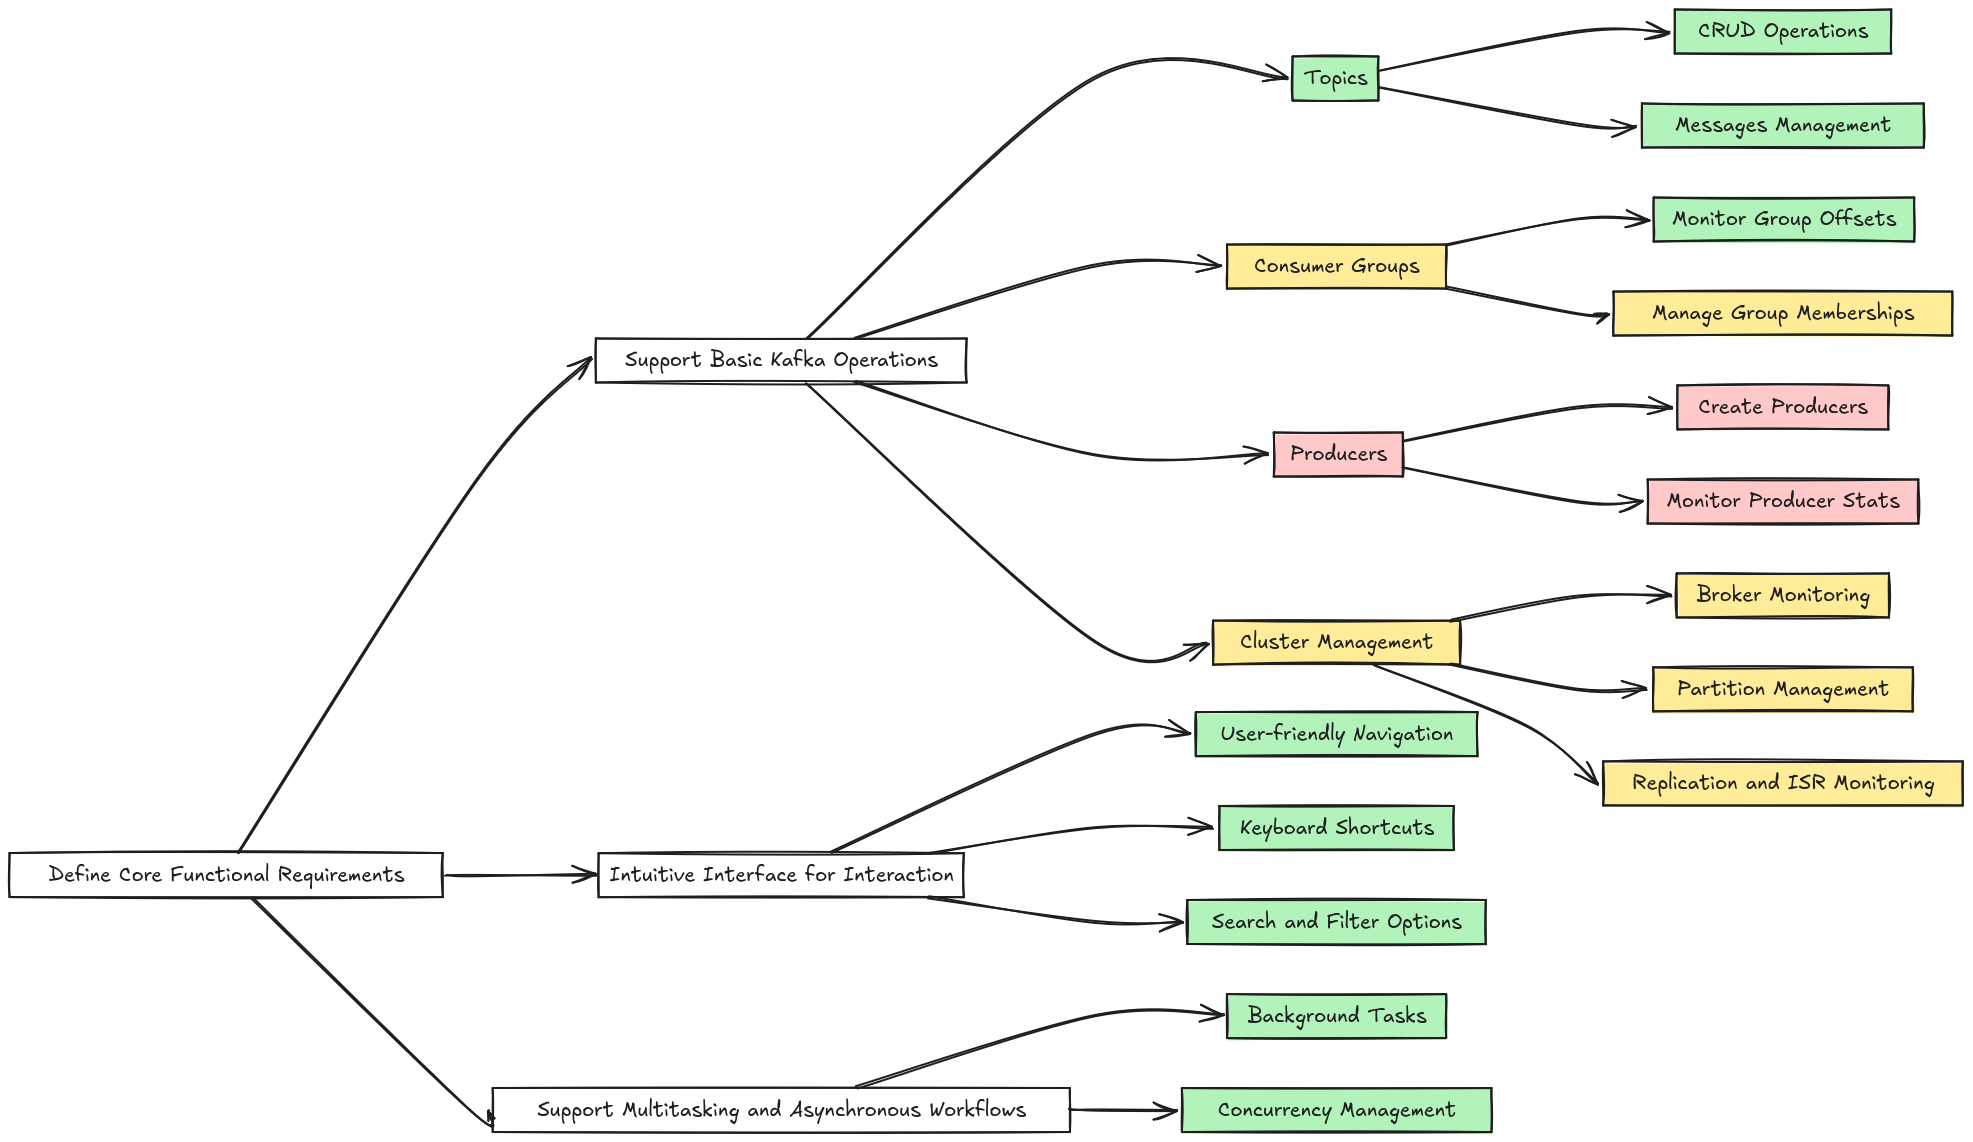
\includegraphics[width=1\linewidth]{imgs/CoreFucntionalRequirementsDiagram.png}
    \caption{Core Functional Requirements}
    \label{fig:core_functional_requirements}
\end{figure}

\begin{itemize}
    \item \textbf{Basic Kafka Operations} — This involves core functionalities for interacting with Kafka. These are features that are essential for any Kafka management utility. I have outlined them separately in Figure~\ref{fig:basic_kafka_operations}, which I will discuss further below.
    
    \item \textbf{Intuitive Interface} — Since I am developing a terminal-based utility for developers who are accustomed to working with terminal applications like Vim, creating user-friendly navigation through versatile keyboard shortcuts is a priority. Additionally, because Kafka is inherently designed for processing large volumes of data, it is essential to provide users with the ability to quickly search for relevant information within a large data stream.
    
    \item \textbf{Multitasking and Asynchronous Workflows} — Again, considering Kafka’s nature of handling significant amounts of data, the fetching process can take time. Ensuring concurrency of processes in this scenario is necessary, and implementing background tasks will be an effective solution.
\end{itemize}

\begin{figure}[htbp]
    \centering
    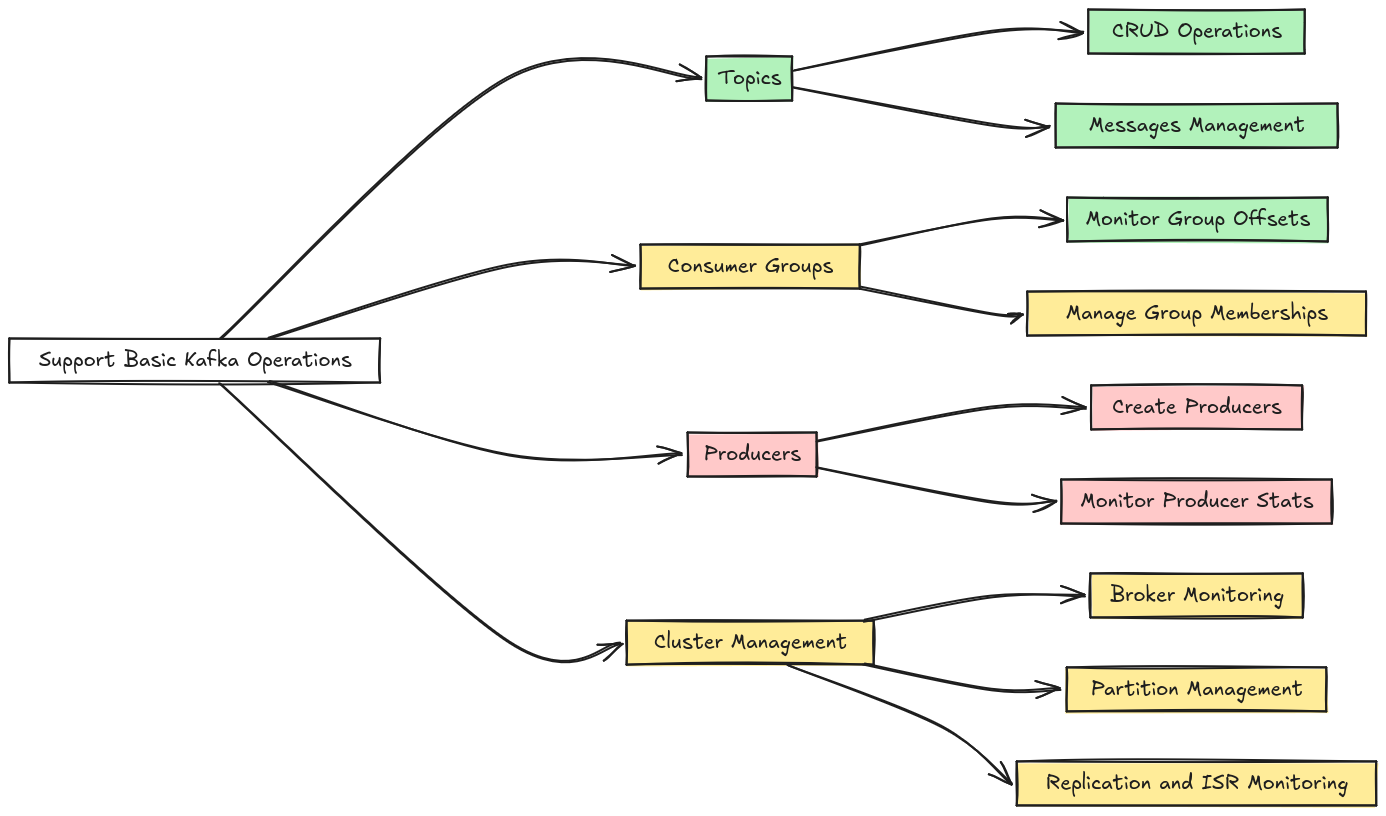
\includegraphics[width=1\linewidth]{imgs/BasicKafkaOperationsDiagram.png}
    \caption{Basic Kafka operations requirements}
    \label{fig:basic_kafka_operations}
\end{figure}

\begin{figure}[htbp]
    \centering
    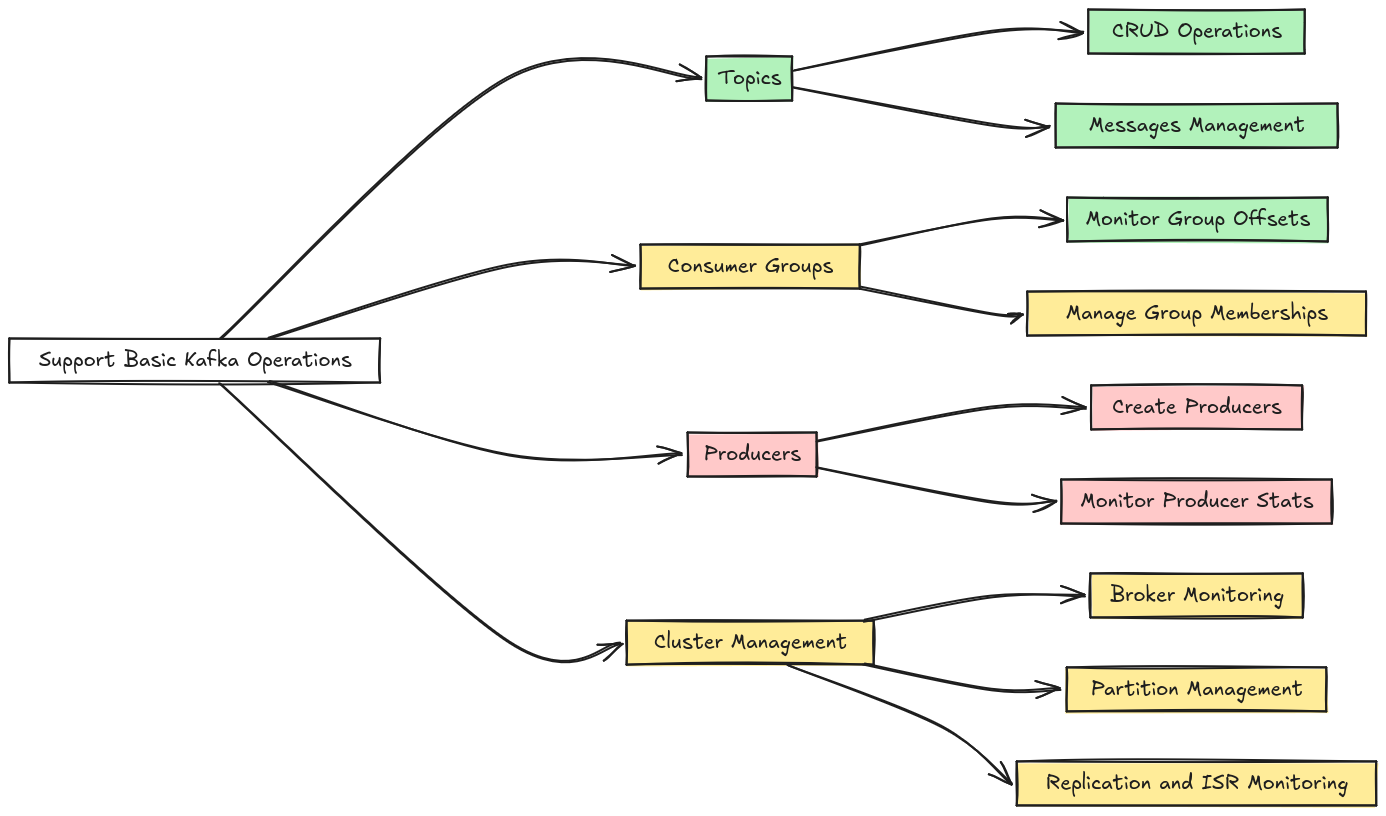
\includegraphics[width=1\linewidth]{imgs/BasicKafkaOperationsDiagram.png}
    \caption{Basic Kafka operations requirements}
    \label{fig:basic_kafka_operations}
\end{figure}

Based on Kafka's architecture (Figure~\ref{fig:kafka_arch}), four primary features come to mind that the management utility must support:
\begin{itemize}
    \item Working with topics
    \item Managing consumer groups
    \item Interfacing with producers
    \item Cluster management
\end{itemize}

\subsection{Interface Structure}

\begin{figure}[htbp]
    \centering
    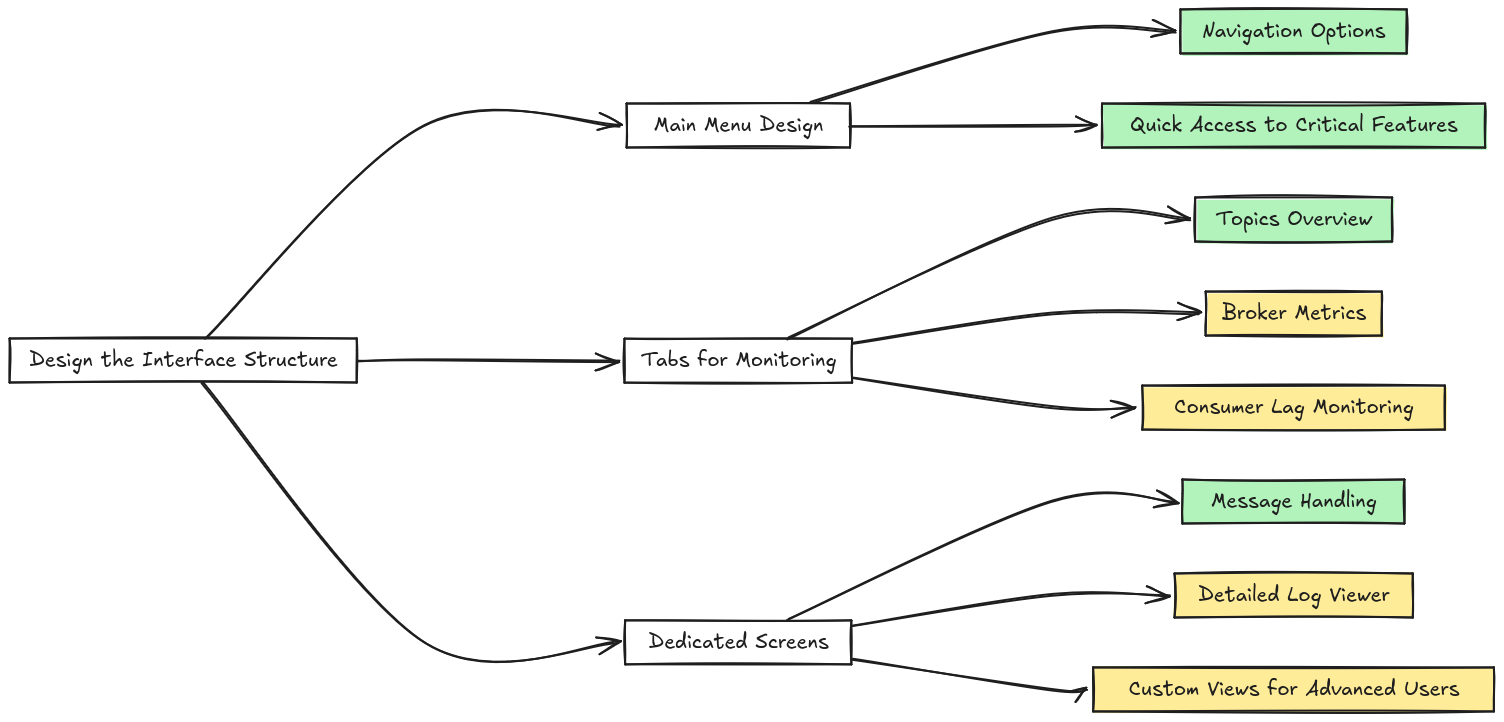
\includegraphics[width=1\linewidth]{imgs/InterfaceDesign.png}
    \caption{Interface design structure}
    \label{fig:interface_design}
\end{figure}

The technologies chosen for UI development significantly influence the design process. Therefore, I want to finalize the interface design before selecting the technology stack. In Figure~\ref{fig:interface_design}, I have highlighted the priority tasks. The most critical aspect is the main menu design, as its navigational capabilities and quick access to core features will determine whether users find the application useful. No matter how powerful the system is, if it’s inconvenient to use, users won’t engage with it.

\subsection{Main Menu Design}\label{subsec:main_menu_design}

From my analysis of LazyDocker in Section~\ref{subsec:ld_analysis}, I identified several features I would like to include in my solution.

Here, I adapt them to suit the needs of my utility:
\begin{itemize}
    \item \textbf{Panes}: Kafka data is naturally suited for display in table format, as most elements can be easily categorized.
    \item \textbf{Hotkeys}: Hotkeys are what make navigation satisfying. They are essential for any TUI utility. I plan to implement a general hotkeys bar and context-specific menus for individual panes. For example, sorting topics by different parameters can be performed using hotkeys.
    \item \textbf{Navigation}: Navigation is equally important. Moving between panes should be intuitive and straightforward. I decided to support navigation not only with \texttt{Tab}/\texttt{Shift+Tab} and arrow keys but also with vim-style hotkeys. Many developers use vim/emacs plugins in their workflows, and it’s enjoyable to have familiar keybindings across the developer environment.
    \item \textbf{Colors}: As mentioned in the analysis, colors play both an aesthetic and functional role. They help highlight important elements and focus the user’s attention where needed. Ideally, I would like to provide customizable palettes, but for the MVP, I will hardcode a basic color palette. If time permits, I will later update it to be configurable.
\end{itemize}

Inspired by LazyDocker, I sketched the following main menu mockup:

\begin{figure}[htbp]
    \centering
    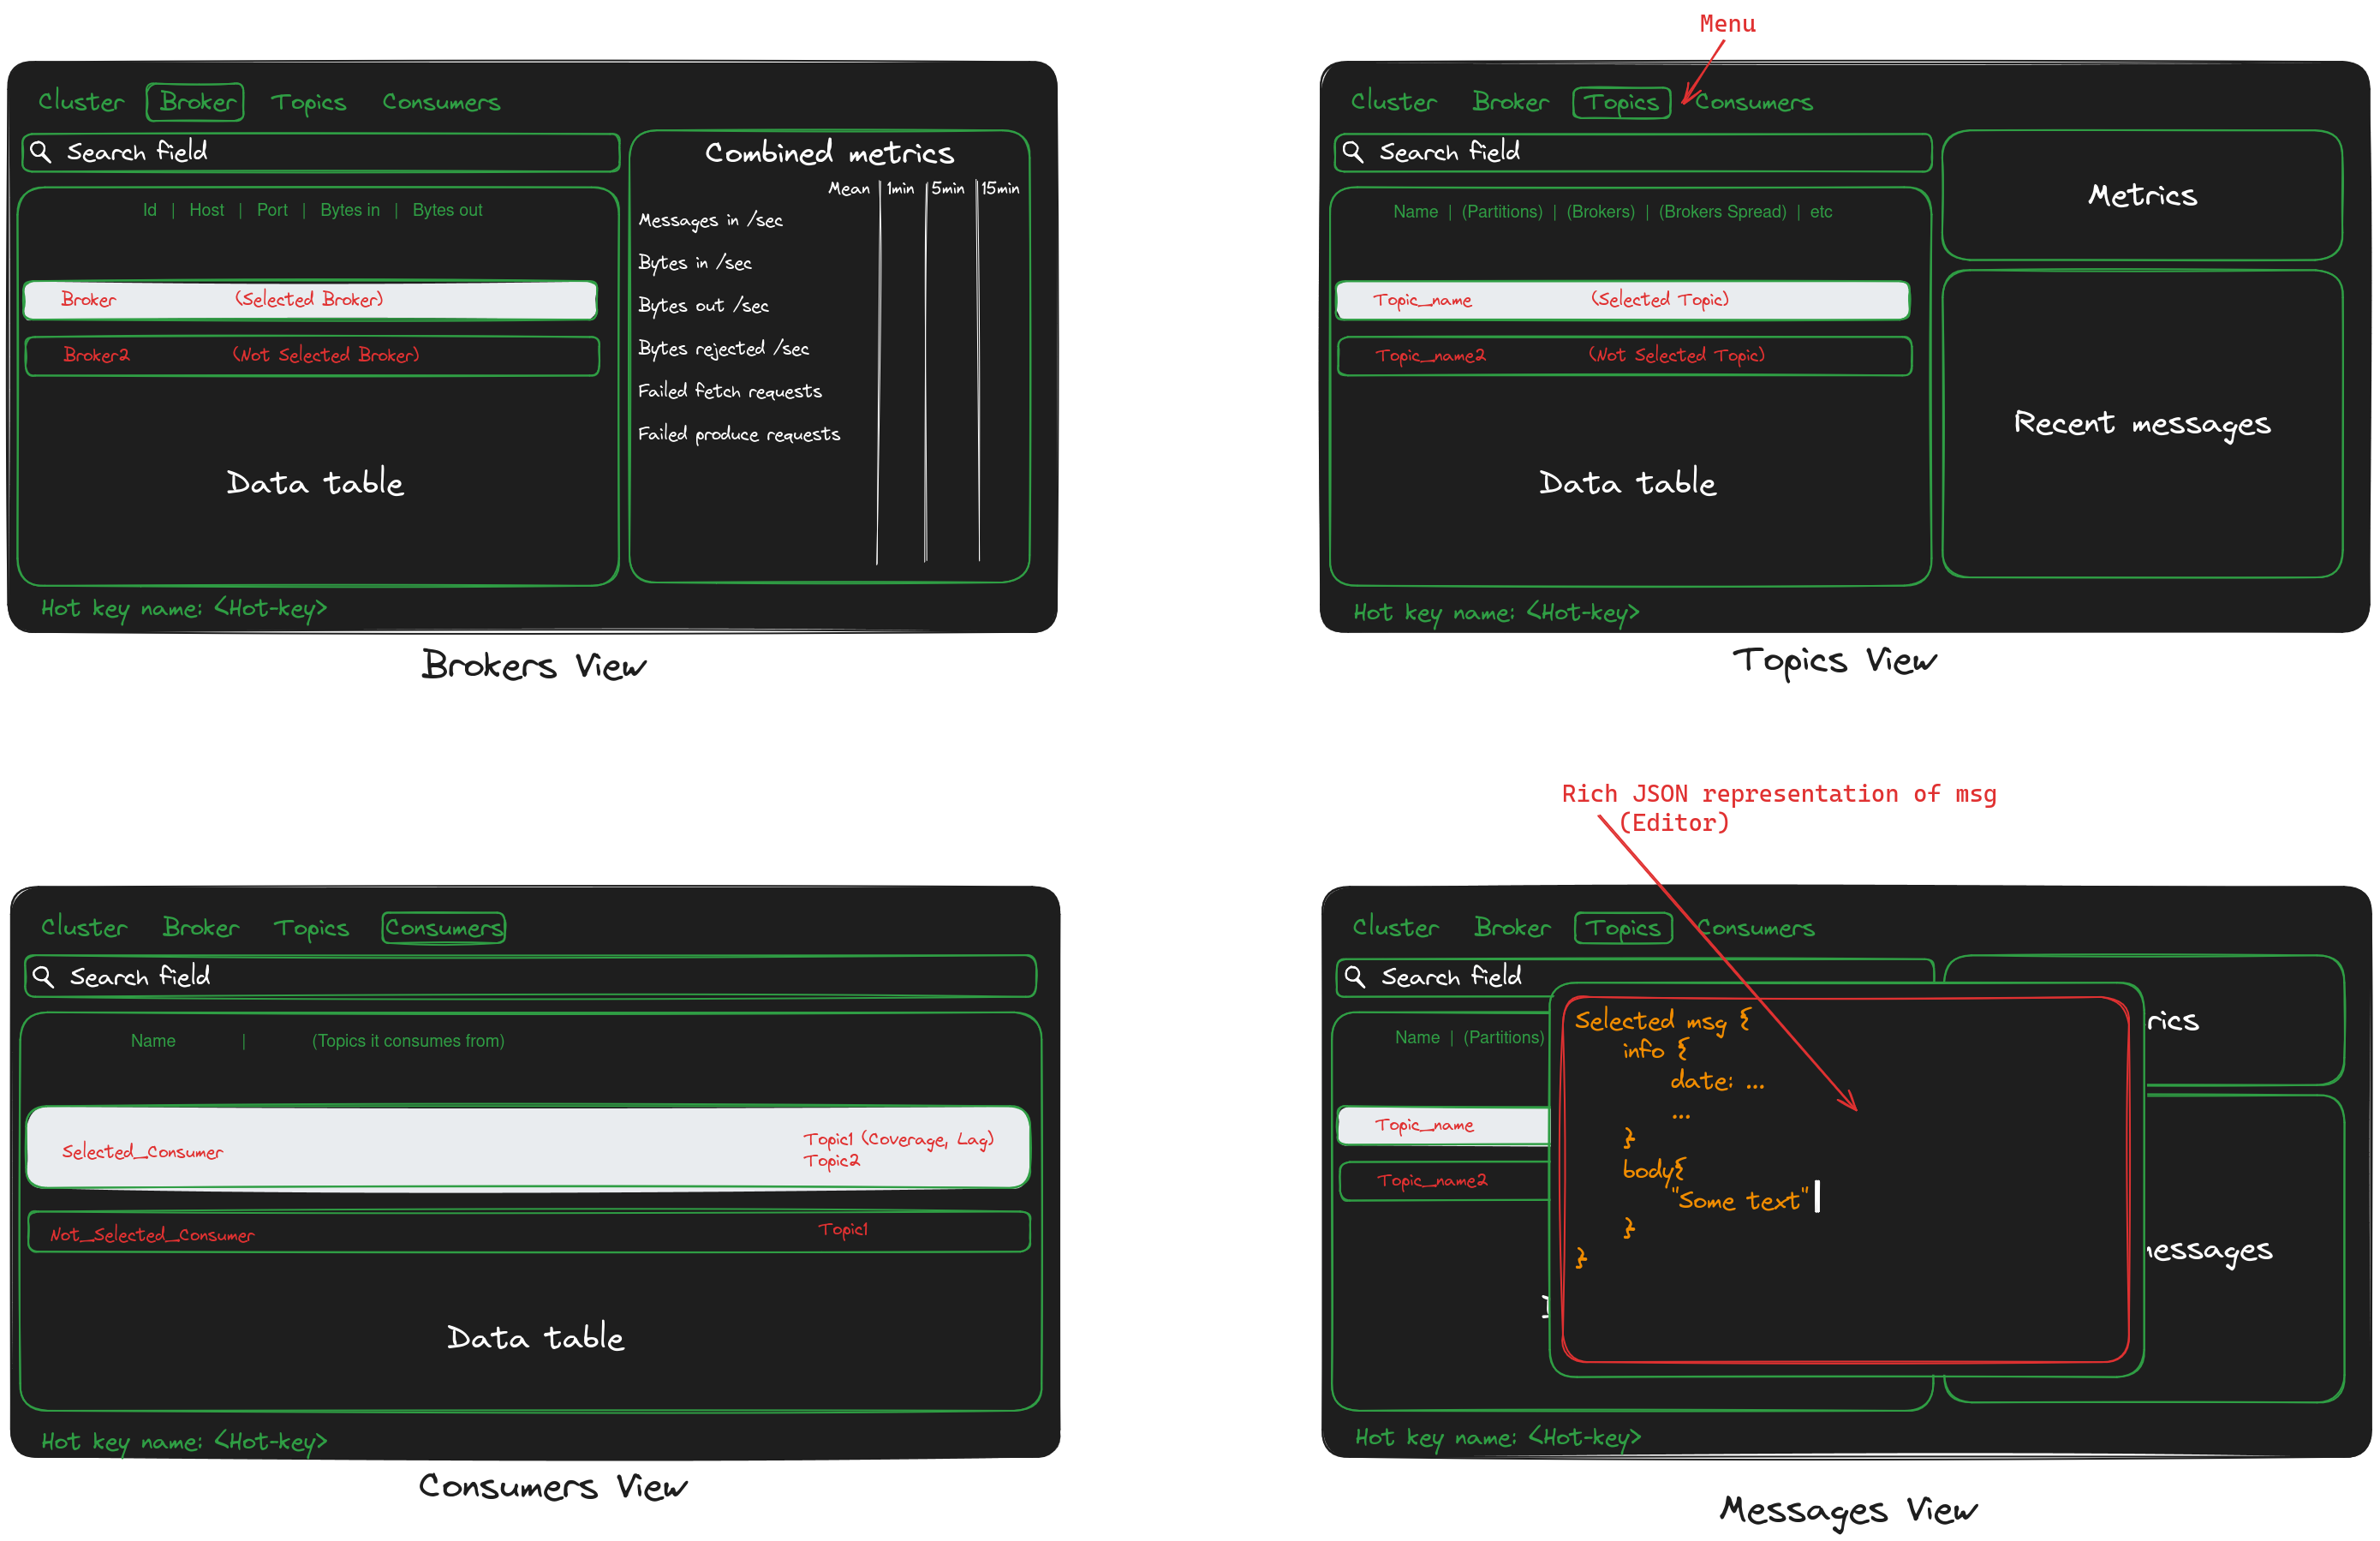
\includegraphics[width=1\linewidth]{imgs/UIMaquette.png}
    \caption{Main menu mockup}
    \label{fig:ui_maquette}
\end{figure}

The first MVP version will only include the topic view and message view. I will discuss these in detail below. For now, a brief note on consumer and broker views: when designing mockups, I drew inspiration from Kafka Manager as a free alternative to Conduktor (which was discussed by Sarah). All views include a data table with various columns. For consumer groups, an initial implementation could include only group names (IDs) and associated topics. The broker screen is intended to track load metrics, so I divided it into two panels—a table panel with general information about each broker and a detailed information panel for the selected broker. In the future, the second panel could include tabs, such as one for rendering load graphs or displaying data loss statistics. To determine their utility, I will consult with my stakeholder.

\begin{figure}[htbp]
    \centering
    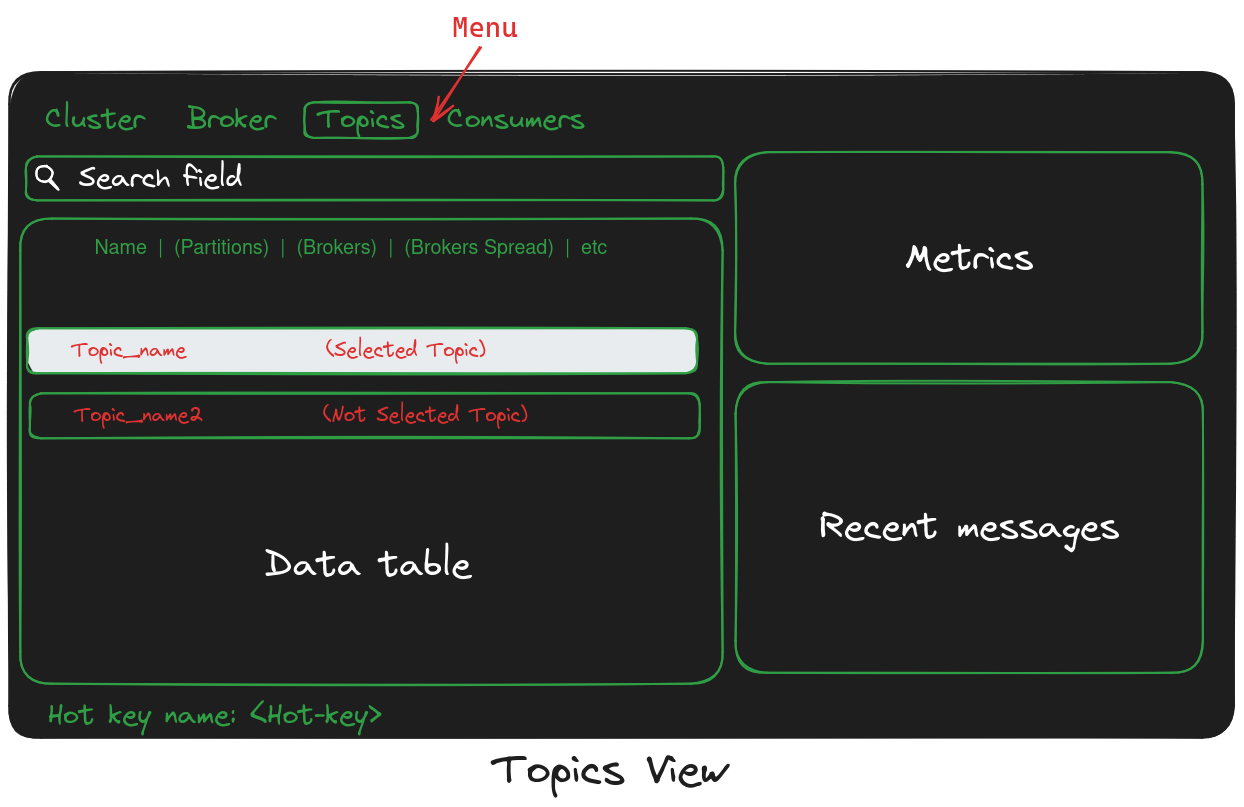
\includegraphics[width=.8\linewidth]{imgs/TopicsScreenDesign.png}
    \caption{Topics screen mockup}
    \label{fig:topics_screen_maquette}
\end{figure}

\textbf{Topics View}: This is the main screen users will interact with most frequently, so it will be the first to be implemented for the MVP. This screen is divided into three panes:
\begin{itemize}
    \item A general pane displaying information about topics in the cluster.
    \item A metrics pane for the selected topic, potentially including graphs for specific time periods. Initially, it will display basic data.
    \item A messages pane showing the last \textit{N} messages in the selected topic. By pressing enter on any topic will open new screen with messages stored in this topic 
\end{itemize}

I think good usability feature that I should include is ability to sort data in the table not only by name, but also but other parameters, as it will definitely speed up users' development process. Also, despite complexity of features proposed by my stakeholder, I should consider them, because it is simply users pain points and creating usability features addressing this points will "sell" my product.

\begin{figure}[htbp]
    \centering
    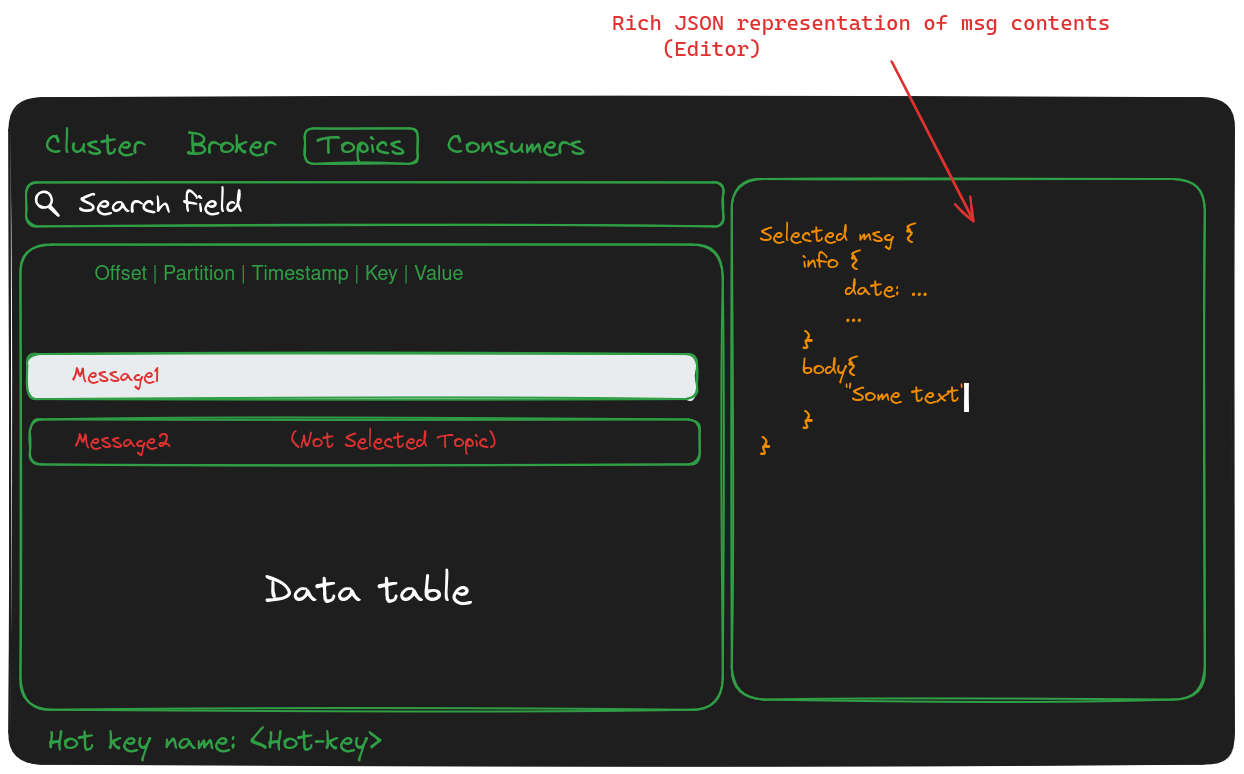
\includegraphics[width=.8\linewidth]{imgs/MessageView.png}
    \label{fig:message_view}
    \caption{Message view}
\end{figure}

Overall, this screen is not drastically different from the topics screen. It presents messages in a tabular format, and when a message is selected, its content can be viewed in an editor displayed on the right side of the screen.

\subsection{Algorithm for Topic Menu Functionality}

Here I will describe how I envision the user interacting with the application, specifically the options they will have when working with topics and the outcomes of selecting each option.

\begin{figure}[htbp]
  \begin{center}
    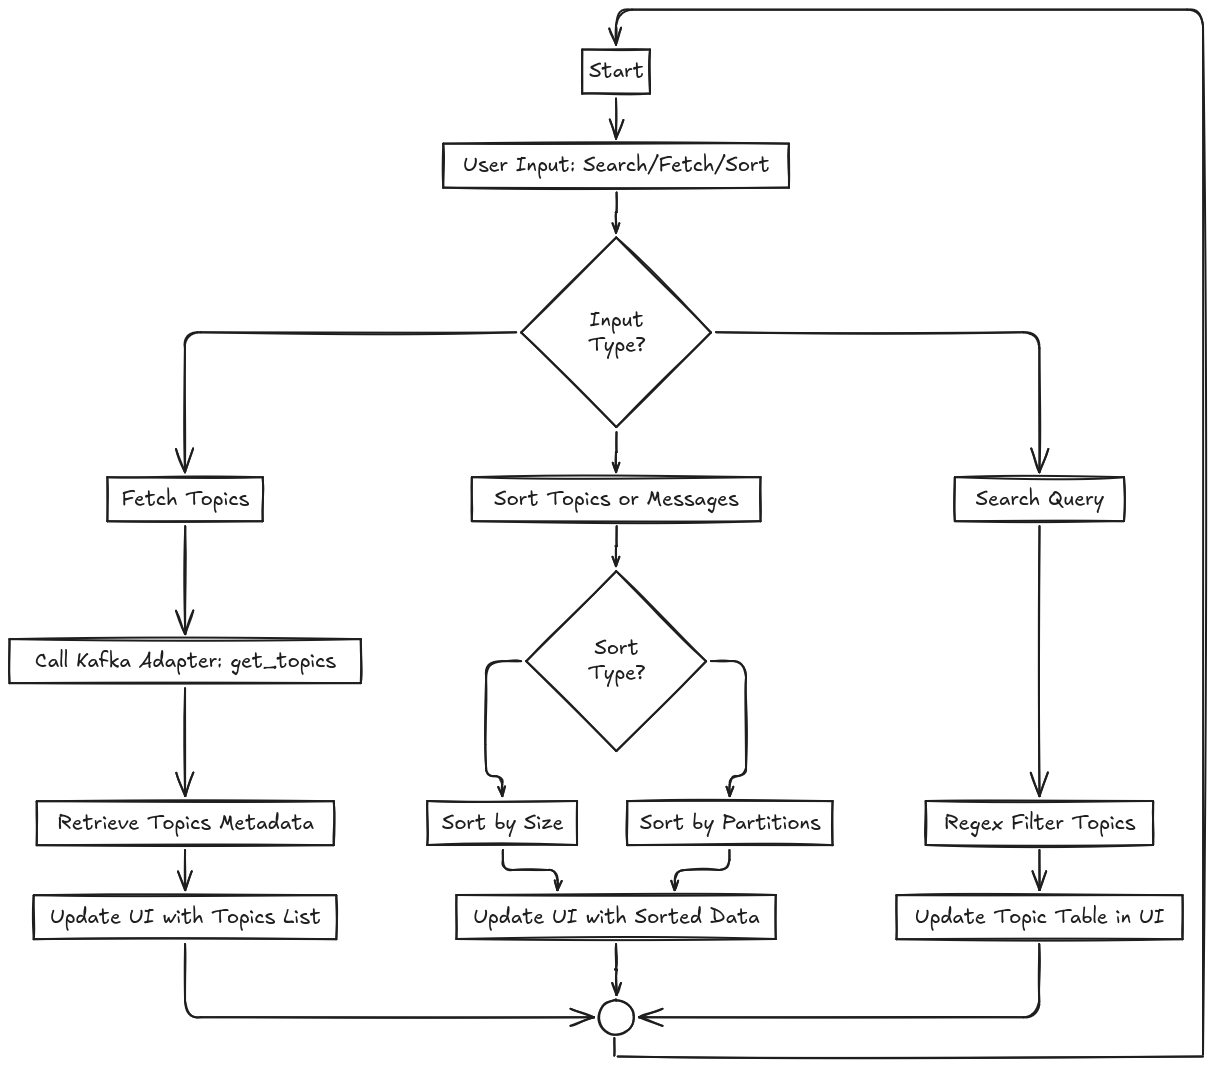
\includegraphics[width=0.95\textwidth]{imgs/TopicsAlgorithm.png}
  \end{center}
  \caption{Algorithm for topic menu functionality.}\label{fig:}
\end{figure}

The figure above illustrates the logical flow of actions a user can take within the topic menu. Each option is designed to provide intuitive and direct access to specific features, ensuring seamless navigation and interaction. For instance:
- Selecting a topic allows the user to view detailed metadata or associated messages.
- Searching filters the list of topics dynamically, enhancing usability in large datasets.
- Sorting offers flexibility to organize topics based on user preferences, such as size or partition count.


\newpage
\subsection{Tech Stack}

Having finalized the two most critical parts of the interface, I can now determine the technology stack. Below, in Figure~\ref{fig:tech_chart}, I have divided the technologies into three categories.

\begin{figure}[htbp]
    \centering
    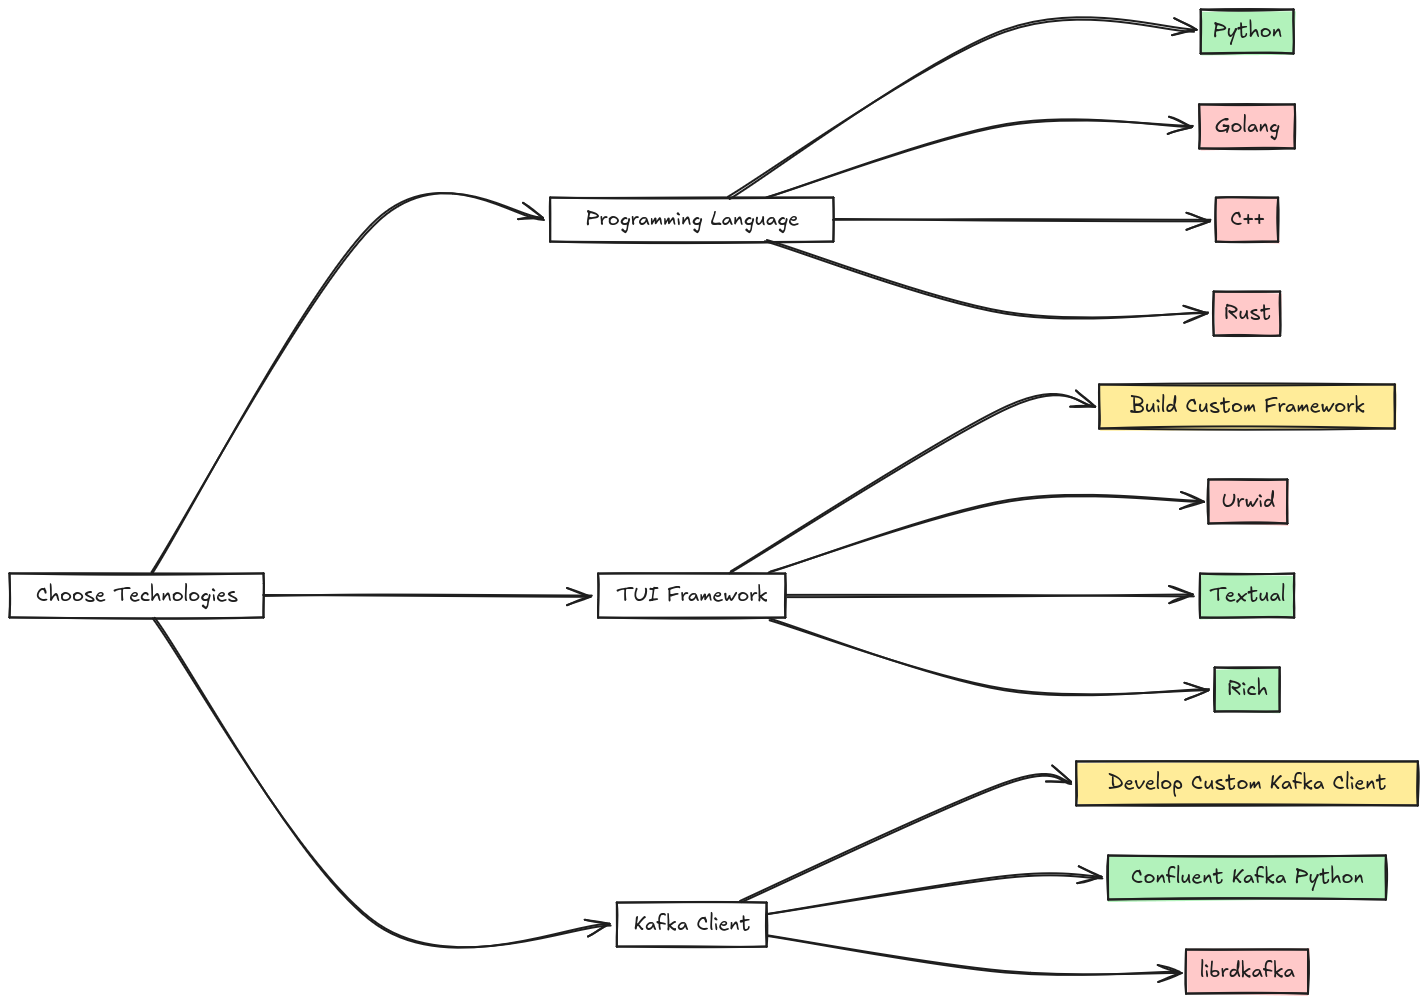
\includegraphics[width=.8\linewidth]{imgs/TechDiagram.png}
    \caption{Technology Stack Overview}
    \label{fig:tech_chart}
\end{figure}

\textbf{Programming Language}: Choosing the programming language is a key decision for the project, as it affects performance, coding style, and the overall development approach. I considered using Rust or Go, but I am not sufficiently experienced with these languages to confidently complete the project within the given timeframe. C++ and C were also on the rejected list for the same reason, even though they are promising choices for creating lightweight, optimized interfaces for Linux command-line environments. These languages, in my opinion, would be excellent for developing a lightweight and optimized terminal interface tailored for Linux users. However, I chose Python instead. Python is both simple to read and powerful, with an extensive library ecosystem. Additionally, I have been working with Python since I was 8 years old, which enables me to estimate tasks with a high degree of accuracy in terms of time. For these reasons, Python will form the foundation of this project.

\textbf{TUI Framework}: The next most important aspect is the user interface. After conducting research, I identified four options. \texttt{Urwid} is a relatively outdated library with sparse documentation, but from the screenshots, it seems to include all the essential components for creating an interface based on my mockups. Its downsides are that it only supports a few terminal emulators and does not run on Windows at all. Then, I discovered \texttt{Textual} and was immediately impressed with its documentation—everything is well-documented, and the library includes numerous widgets required for developing a terminal interface. Additionally, \texttt{Textual} claims to be nearly universal, running seamlessly across different environments while maintaining consistent appearance, which is crucial for a good TUI utility. You may notice that I marked not only \texttt{Textual} as my preferred framework but also another option—\texttt{Rich}. Technically, \texttt{Rich} was created by the authors of \texttt{Textual} and integrates fully with it, so I consider them as a single framework, even though they are technically distinct libraries.

I also highlighted the option of building a custom framework in yellow. This option is highly unlikely but not impossible. If \texttt{Textual} fails to meet my needs, I may have to explore other options or develop a solution myself, which would require significantly more time. However, within the scope of this coursework, it is unlikely that I will pursue this route.

\textbf{Kafka Client}: The wrapper cannot function without connecting to the system itself. I found two options, but \texttt{confluent\_kafka} has better and simpler documentation, along with a more active GitHub repository. Therefore, I chose this library. As with the TUI framework, creating a custom framework is always an option, but it is an extremely complex task and is unlikely to be part of this coursework.

\subsection{Testing and Debugging}

\begin{figure}[htbp]
    \centering
    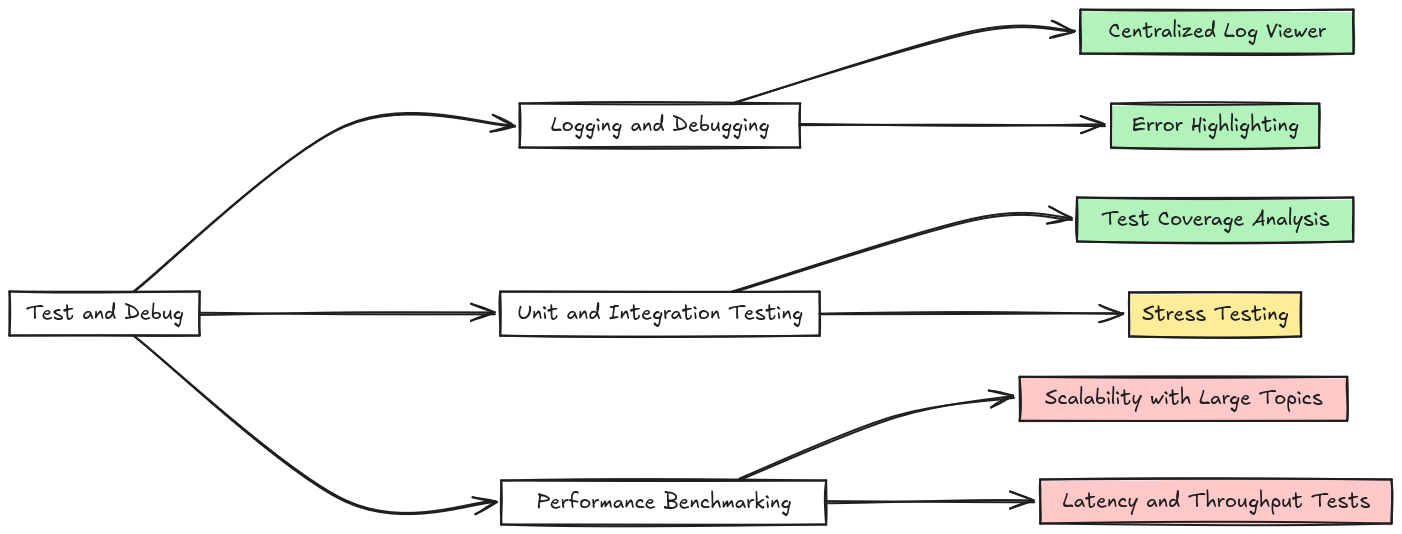
\includegraphics[width=1\linewidth]{imgs/TestDebugDiagram.png}
    \caption{Testing and Debugging Plan}
    \label{fig:test_debug}
\end{figure}

It is crucial to establish the testing boundaries early on to avoid spending excessive time on non-critical areas. Logging is an essential feature for any project, as debugging without logs can become a nightmare. The same applies to error highlighting—errors should be highlighted in the logs to make them easier to locate in large log files. For the evaluation phase, I need to provide proof of testing, and since I plan to use a Test-Driven Development (TDD) approach during development, tracking the percentage of code covered by tests will be helpful.

Since this is an MVP, stress testing and scalability are not critical at this stage. The MVP's goal is to function and demonstrate the system's capabilities to the stakeholders. Like a sketch in drawing, an MVP provides sufficient understanding but is almost never the final extensible solution. Therefore, I decided not to include performance benchmarking in the initial releases, and stress testing will only be conducted if time allows.

\begin{table}[h!tbp]
\centering
\renewcommand{\arraystretch}{1.3} % Adjust row spacing for readability
\begin{tabular}{|l|p{10cm}|}
\hline
\textbf{Data Type} & \textbf{Description and Justification} \\ \hline
User Feedback & Collecting user feedback is crucial, as it allows to identify pain points  \\ \hline
Performance Metrics & Measure response times, latency, and throughput under normal and stressed condition. It helps validate performance efficiency and reliability. \\ \hline
Log & Logs are very convenient way to trace bugs. It will help in enhancing Fault Tolerance and Maintainability. \\ \hline
User Interaction Tracking & Analyze usage patterns through clickstream data or heatmaps to optimize UI and improve Usability. (But in my project I probably won't do it, as it is extremley hard to do) \\ \hline
Regression Testing Results & I will automate test suites and collect pass/fail results after each itteration and in post development phase. It helps to be sure, that system aligns with my vision (But it only works if tests are good). \\ \hline
System Resource Utilization & I could monitor CPU, memory, and network usage to identify and resolve performance bottlenecks. \\ \hline
Benchmark Comparisons & Compare system performance metrics to industry standards as I don't have any better source. \\ \hline

\end{tabular}
\caption{Post-Development Data}
\label{tab:post_dev_data}
\end{table}

\newpage
\subsection{Release and Support}
\begin{figure}[htbp]
    \centering
    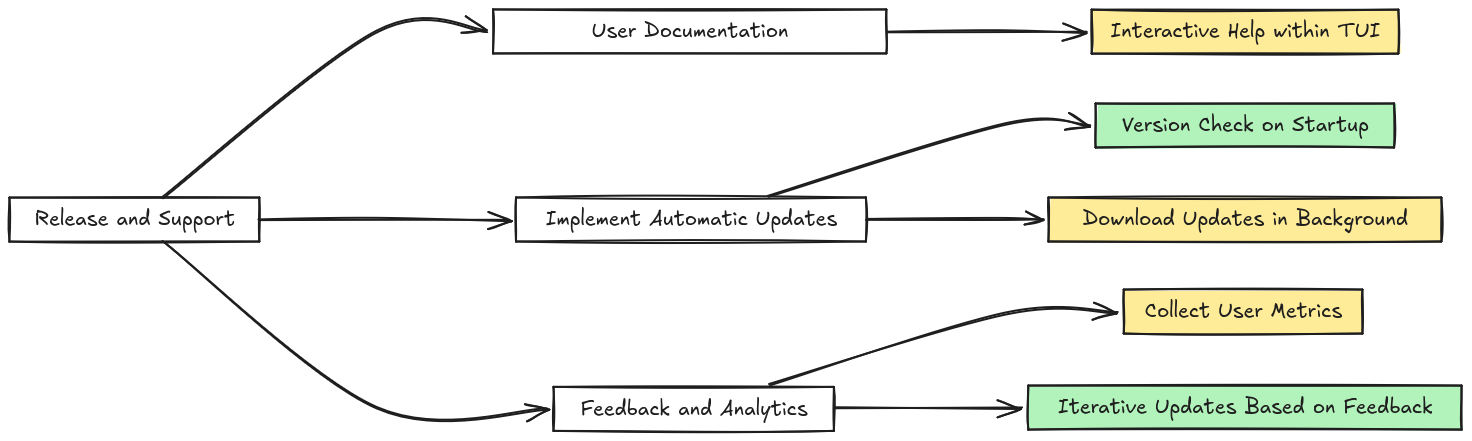
\includegraphics[width=1\linewidth]{imgs/ReleaseSupportDiagram.png}
    \caption{Release and Support Plan}
    \label{fig:release_support}
\end{figure}

Supporting the product during and after development is as important as the development itself. I divided this section into three parts: documentation, updates, and feedback/analytics.

\textbf{Documentation}: Documentation is a critical part of any project involving multiple developers. However, since this is a school project with limited time, and good documentation is typically time-intensive, I will focus on inline code comments and Python's built-in \texttt{pydoc} library (\url{https://docs.python.org/3/library/pydoc.html}), which converts comments in the code into well-formatted HTML and CLI manual pages.

\textbf{Updates}: Tracking application versions is good practice. In the final application, I could offer users the option to update the package when new versions are released. However, this task is not essential for the MVP, and I find it challenging to estimate the time required for implementing this functionality. Thus, this task will be deferred until after the core features of the first release are completed.

\textbf{Feedback and Analytics}: These are two things that help improve the application. In this project, I work iteratively with my stakeholders, collecting feedback to refine the application. I also believe that assessing an application's performance requires more than just feedback—quantifiable metrics are needed for a more accurate evaluation. However, collecting metrics from the beginning, before acquiring any users, is relatively pointless and is not critical for developing a good MVP. Therefore, assuming a small number of initial users (stakeholders), I plan to implement this feature in future releases.

\section{Structure of the Solution}

We have already discussed the interface layout in Section~\ref{subsec:main_menu_design}, but now, based on the technical decisions—particularly the choice of programming language—we can consider the design of the backend, which is the core of the application responsible for processing and transferring data from Kafka to the frontend.

In real-world development, the Domain-Driven Design (DDD) approach is widely used. DDD not only helps structure the project but also facilitates communication between technical teams and stakeholders. My stakeholders are developers, so they can generally understand technical discussions. However, using DDD will allow us to "speak the same language." For example, instead of saying, "That thing in Kafka that stores messages," I can simply say "Topic," and everyone will understand. This is the main advantage of DDD—it aligns terminology and simplifies collaboration. Additionally, DDD makes it easier to structure the project architecture.

To understand the subsequent sections, it is essential to define what a design pattern is. A \textbf{design pattern} is a frequently used solution to a common problem encountered during software architecture design. Design patterns serve as guidelines for structuring your code in a way that promotes flexibility, reusability, and scalability. To explain it in simple terms, a design pattern is like a blueprint or template for solving a specific problem. For further details, see \url{https://refactoring.guru/design-patterns/what-is-pattern}.

For the application, I decided to base the architecture on the MVC (Model-View-Controller) design pattern. MVC is a popular method of organizing code. The central idea of MVC is that each section of your code has a distinct purpose:
\begin{itemize}
    \item \textbf{Model}: Handles the data and business logic of the application. It fetches and processes data, typically from Kafka in our case.
    \item \textbf{View}: Manages the display and presentation of the data. For this project, it will be responsible for the terminal user interface (TUI).
    \item \textbf{Controller}: Acts as the intermediary between the Model and View. It processes user input, updates the Model, and refreshes the View accordingly.
\end{itemize}

The primary advantage of MVC is that it separates concerns, making the code easier to maintain and scale. Moreover, since I am following a Test-Driven Development (TDD) approach, MVC naturally supports testing by isolating the logic in the Model and keeping the View and Controller relatively lightweight.

\subsection{MVC use}

\begin{figure}[htbp]
  \begin{center}
    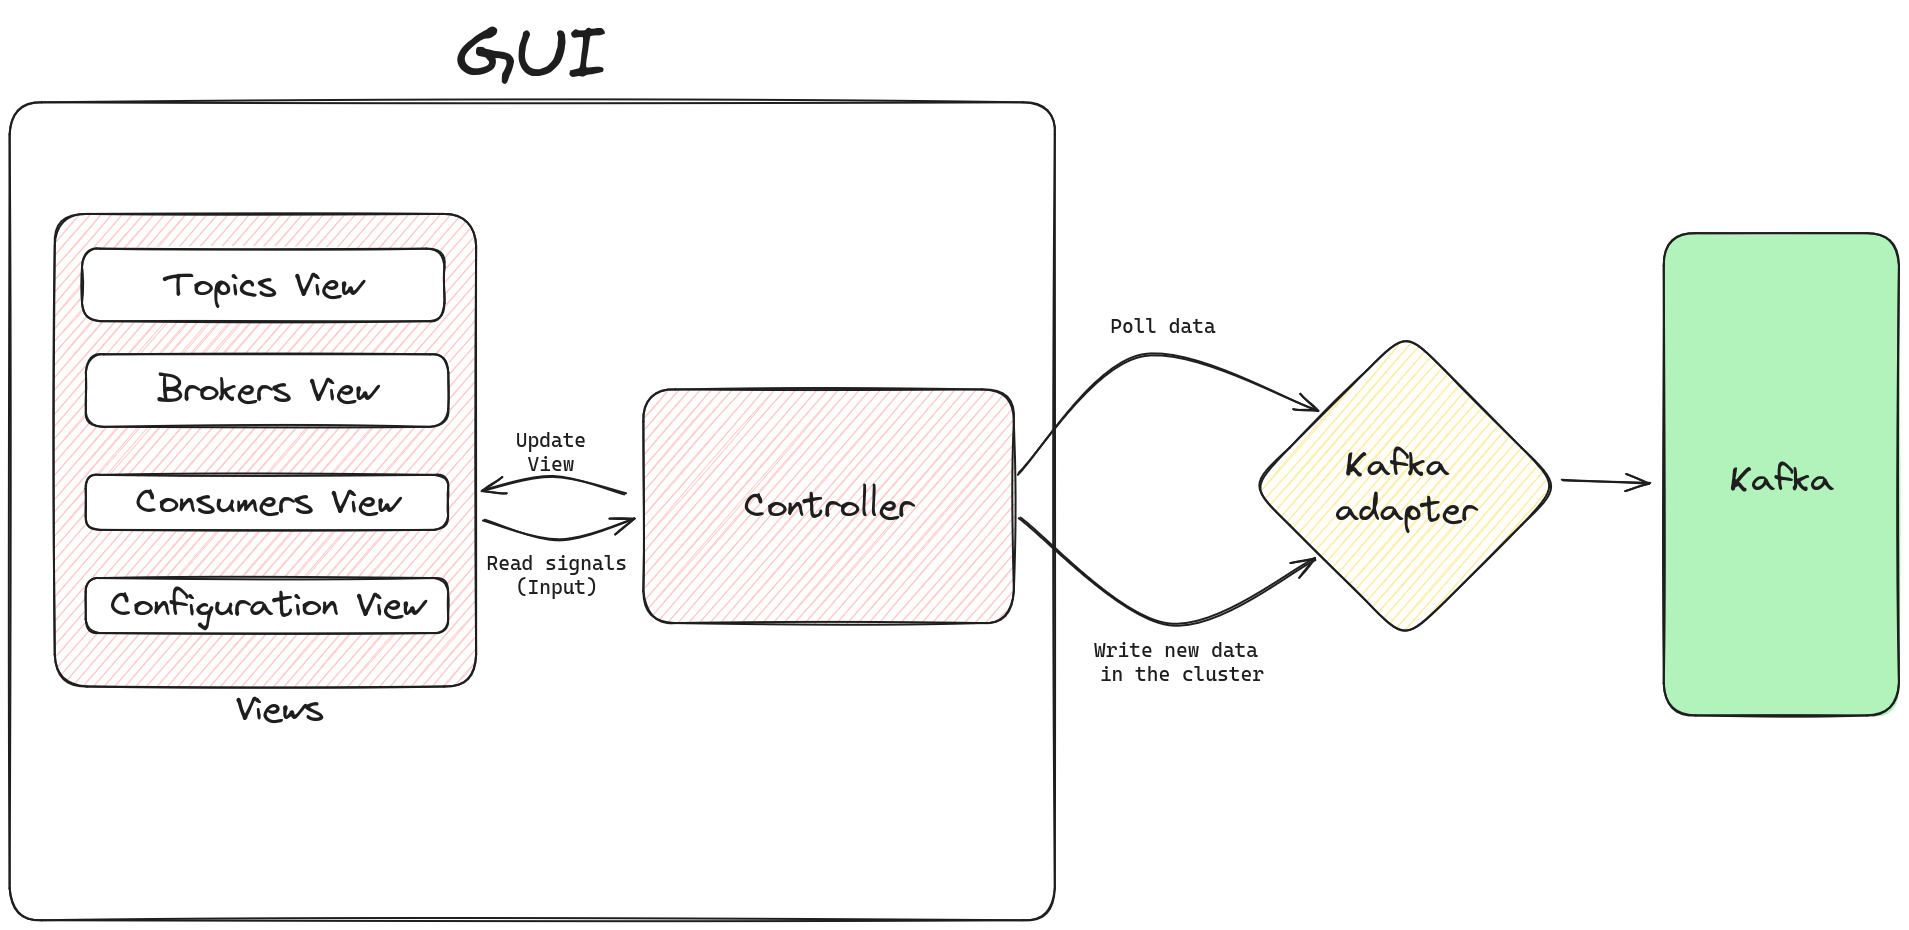
\includegraphics[width=0.95\textwidth]{imgs/InitialArchitecture.png}
  \end{center}
  \caption{}\label{fig:mvc_diagram}
\end{figure}

In Figure~\ref{fig:mvc_diagram}, I present a high-level overview of how I plan to implement the MVC pattern for this project. Let us briefly examine each component:

\subsubsection{Model}

The Model will handle all interactions with Kafka. This includes:
\begin{itemize}
    \item Fetching metadata (e.g., list of topics, consumer groups).
    \item Reading and writing messages to and from topics.
    \item Monitoring cluster health and performance metrics.
\end{itemize}

\subsubsection{View}

The View is responsible for rendering the user interface. I will use the \texttt{textual} and \texttt{rich} libraries to build an intuitive terminal-based UI. The main components include:
\begin{itemize}
    \item \textbf{Main Menu}: Displays the core features and navigational options.
    \item \textbf{Data Tables}: For presenting topics, messages, and metrics in an organized format.
    \item \textbf{Message Viewer}: Provides a detailed view of individual messages, basically editor.
\end{itemize}

\subsubsection{Controller}

The Controller will handle user inputs (e.g., keyboard shortcuts, navigation commands) and translate them into actions. For example:
\begin{itemize}
    \item If a user selects a topic, the Controller will fetch the corresponding messages via the Model and update the View.
    \item If a user deletes a topic, the Controller will invoke the appropriate method in the Model and refresh the View.
\end{itemize}

By centralizing input handling in the Controller, we ensure that the business logic in the Model remains decoupled from the presentation logic in the View.

\subsection{Architecture}

\begin{figure}[htpb]
  \begin{center}
    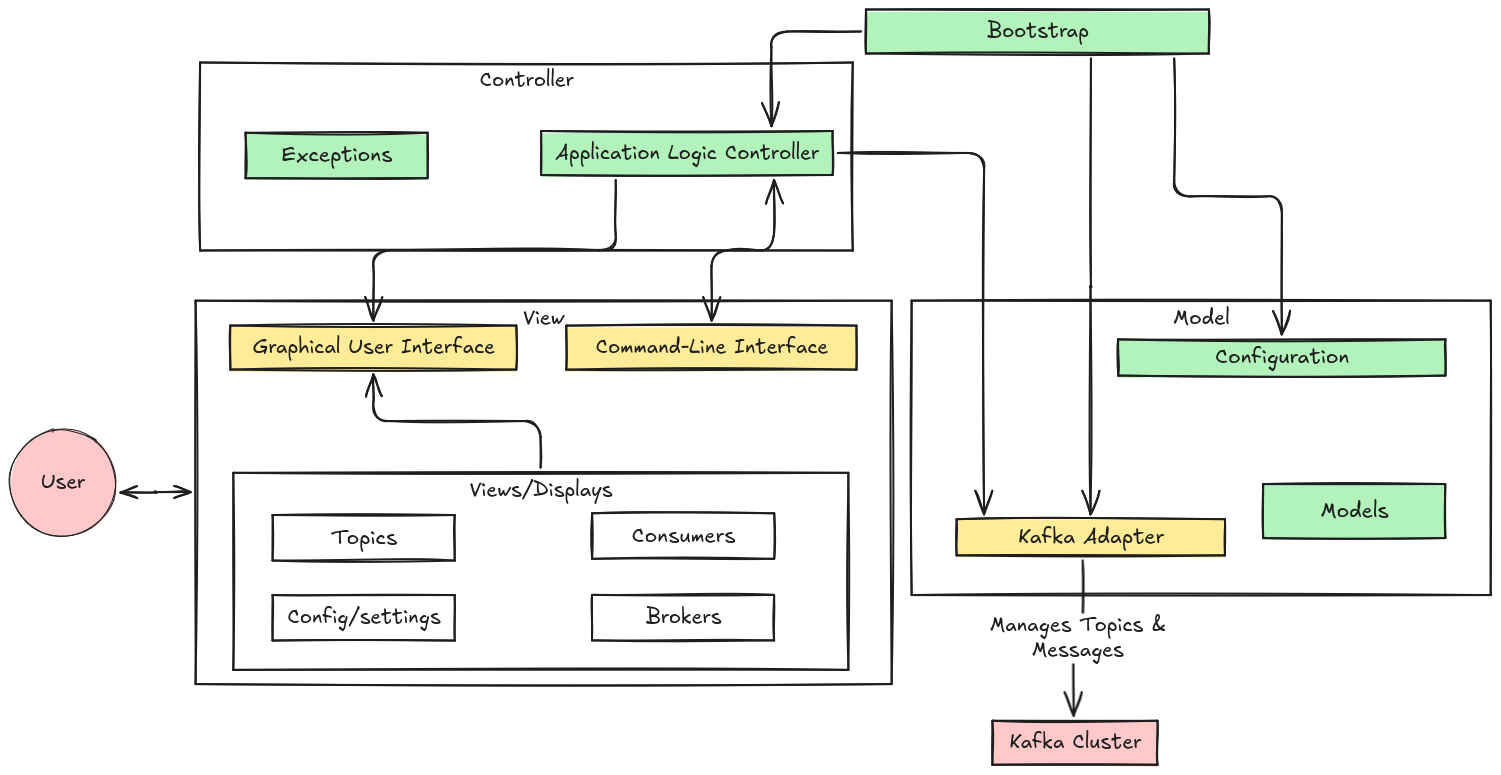
\includegraphics[width=0.95\textwidth]{imgs/ArchitectureDetailed.png}
  \end{center}
  \caption{Detailed Architecture Overview}\label{fig:detailed_arch}
\end{figure}

After spending some time sketching out ideas, I arrived at this architecture. All components are divided into three categories and follow the MVC pattern. The system is initialized from a bootstrap class, and public objects are stored in this class to allow them to be accessed from anywhere within the system.

\begin{itemize}
  \item \textbf{Controller}: The brains of the application, responsible for processing and dispatching signals to other systems. Includes:
    \begin{itemize}
      \item \textbf{Exceptions}: A set of custom exceptions that the system will throw in case of errors. While not critical for an MVP, they will enhance user feedback when reporting bugs and speed up development by clarifying error-handling logic.
    \end{itemize}

  \item \textbf{Model}: Holds all the data and the classes needed to access this data. Includes:
    \begin{itemize}
      \item \textbf{Configuration Class}: A class that stores configurable parameters. During initialization, it loads data like the Kafka host, login, and password from configuration files or environment variables. Centralizing all configurable parameters makes refactoring simpler by clearly separating responsibilities
      \item \textbf{Models}: Specifications for the data models the system works with. Essentially, these are data classes used to validate incoming and outgoing data
      \item \textbf{Adapters}: Adapters follow a design pattern and act as an interface to external systems. Multiple adapters could be supported, but for the MVP, I plan to focus on Kafka. The structure of the Kafka adapter is detailed in subsection~\ref{subsec:Adapter}
    \end{itemize}

  \item \textbf{View}: The frontend of the application, containing the views or displays that the user interacts with. The controller reads the user input, processes it, and displays the appropriate information through the views. There could be multiple views (e.g., web, CLI, native app), each with a different implementation but consistent functionality. I plan to implement in the first release a Topics view (TUI) and configureable parameter inputs (CLI)
\end{itemize}

\subsection{Models}

In the first release, I will focus on Topics and Messages. Therefore, the primary models will be \texttt{Topic} and \texttt{Message}. However, given that Kafka topics are divided into partitions, and messages reside in partitions rather than directly in topics, it makes sense to add \texttt{Partition} as a model. This simplifies data parsing and supports future functionality.

\begin{figure}[htbp]
  \begin{center}
    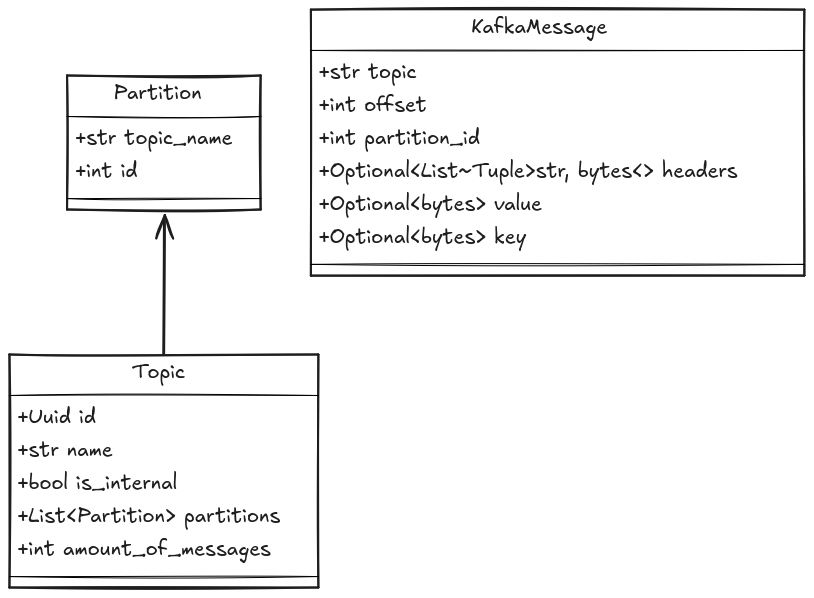
\includegraphics[width=0.7\textwidth]{imgs/Models.png}
  \end{center}
  \caption{Model Structure}\label{fig:models}
\end{figure}

The models are based on Kafka objects and initially use Kafka's native data types to avoid unnecessary data conversion overhead.

\newpage
\subsection{Adapter}\label{subsec:Adapter}

An adapter is an interface, and every interface has a specification. For example, an adapter converting from a UK plug to a European socket must always take three prongs as input and produce two as output. Regardless of the internal implementation of the adapter it follows this "rules". Similarly, here, I use an abstract class to specify the adapter interface for Kafka.

The abstract class defines the abstract methods that the business logic will interact with. An adapter class will inherit from this abstract class and provide concrete implementations of these methods. This concept is easier to understand when viewed in Figure~\ref{fig:AdapterUML}.

\begin{figure}[htpb]
    \centering
    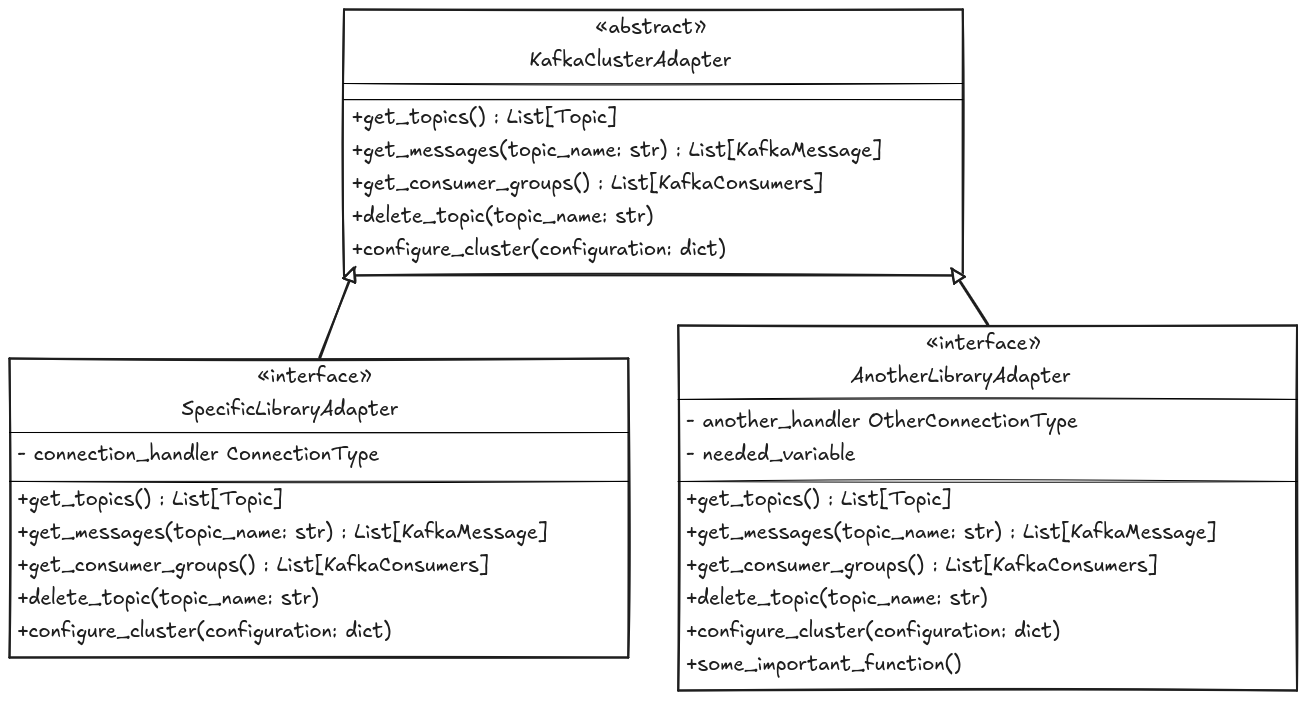
\includegraphics[width=1\linewidth]{imgs/AdapterUML.png}
    \caption{Adapter Example}\label{fig:AdapterUML}
\end{figure}

I have outlined several potential methods for the system, but for the first release, I will focus on implementing only two: \texttt{get\_topics()} and \texttt{get\_messages()}.

\chapter{Development}
\section{Preparation}

\subsection{Folder Structure}

\begin{figure}[htbp]
\centering
\begin{BVerbatim}
.
├── kandy_kafka/
│   ├── adapters/
│   │   ├── __init__.py
│   │   └── kafka_adapter.py
│   ├── gui/
│   │   ├── __init__.py
│   │   ├── controller.py
│   │   └── views
│   │       └── topic_view.py
│   ├── bootstrap.py
│   ├── config.py
│   ├── logger.py
│   └── models.py
├── tests/
├── docker-compose.kafka.yaml
├── kandy.py
├── LICENSE
├── Makefile
├── pyproject.toml
└── README.md
\end{BVerbatim}
\caption{Project folder structure}
\end{figure}

For this project, I chose to use the `poetry` dependency manager instead of the standard `pip`. `Poetry` simplifies the management of environments and dependencies but requires a specific project structure. For instance, the code must reside in a folder named after the project unless specified otherwise in the configuration file. Additionally, the root directory must contain a \texttt{README.md} file, along with all Git-related files and scripts (e.g., test scripts). 

The core code is stored in the \texttt{kandy\_kafka/} folder. Below, I describe the purpose of each file and folder:

\begin{itemize}
  \item \textbf{README.md}: Contains project information, including a description, requirements, and installation instructions.
  \item \textbf{pyproject.toml}: Used by \texttt{poetry} to define dependencies and project metadata. A detailed version is available in Appendix~\ref{appendix:libs}.
  \item \textbf{Makefile}: A script for automating tasks using the \texttt{make} tool\footnote{\textbf{Make} is a command-line tool for executing tasks defined in a configuration file.}.
  \item \textbf{LICENSE}: Since I plan to open-source this project after my A-levels, I included the GPL license to guarantee end-user freedoms to run, study, share, and modify the software.
  \item \textbf{kandy.py}: The entry point of the application that the user will run.
  \item \textbf{docker-compose.kafka.yaml}: This file specifies the configuration for Docker Compose, which I use to set up a Kafka environment for testing.
  \item \textbf{kandy\_kafka/}: Contains the core project code:
    \begin{itemize}
      \item \textbf{adapters/}: Holds adapter and repository files.
      \item \textbf{gui/}: Contains views and the controller.
      \item \textbf{bootstrap.py}: Defines the application startup logic.
      \item \textbf{config.py}: Handles external configuration parameters.
      \item \textbf{logger.py}: Manages logging setup using Python's built-in \texttt{logging} library.
      \item \textbf{models.py}: Contains data models, represented as Python \texttt{dataclasses}.
    \end{itemize}
  \item \textbf{tests/}: Directory containing automated tests.
\end{itemize}

This folder structure enforces separation of concerns, helping to write cleaner, maintainable code.

\subsection{Libraries}

The latest version of \texttt{pyproject.toml} is provided in Appendix~\ref{appendix:libs}. For now, I have included the following libraries:

\begin{itemize}
  \item \textbf{pytest}: A testing framework for creating and running test cases efficiently.
  \item \textbf{pydantic}: A data validation library
  \item \textbf{confluent-kafka}: A library chosen during the design phase to handle Kafka cluster communication.
  \item \textbf{urwid}: Although I initially selected \texttt{textual} as the primary library for GUI development, I decided to prototype one view using \texttt{urwid} for comparison and learning purposes. This experiment will help refine my choice.
\end{itemize}

\newpage

\section{Coding}
\subsection{Project Skeleton}

I began by creating the skeleton of my application. This involves defining the classes and functions I plan to use, without implementing the actual logic yet.


\begin{code}
  \begin{minted}[fontsize=\small, breaklines]{Python}
# kandy_kafka/logger.py

import logging


def setup_logger(log_level: str):
    """
    Set up the logger for the application.
    """
    # Remove all handlers associated with the root logger object.
    for handler in logging.root.handlers[:]:
        logging.root.removeHandler(handler)

    logging.basicConfig(
        format="%(asctime)s,%(msecs)d %(levelname)-8s [%(filename)s:%(lineno)d] %(message)s",
        datefmt="%Y-%m-%d:%H:%M:%S",
        level=log_level,
        filename="kandy_kafka.log",
    )
  \end{minted}
\caption{Logger setup function}
\end{code}

For logging, I reused a function from one of my previous projects, making minor adjustments. The function initializes a logger and formats the log output to be written to a file with name \texttt{kandy\_kafka.log} instead of \texttt{stdout}.


\begin{code}
  \begin{minted}[fontsize=\small]{Python}
# kandy_kafka/config.py

import os
from kandy_kafka import logger


class Config:
    LOGGING_LEVEL: str

    KAFKA_HOST: str
    KAFKA_PORT: int

    def __init__(self) -> None:
        self.LOGGING_LEVEL = os.getenv("LOGGING_LEVEL", "INFO")
        logger.setup_logger(self.LOGGING_LEVEL)

        self.KAFKA_HOST = os.getenv("KAFKA_HOST", "localhost")
        self.KAFKA_PORT = int(os.getenv("KAFKA_PORT", 9092))
  \end{minted}
\caption{Configuration class}
\end{code}

Next on the line was configuration. This is a class with public fields that are filled from environment variables or configuration files at application startup. The configuration contains fields for the Kafka cluster host and port, which will later be used in the Kafka adapter. I also included the logging level in the configuration, allowing the application to adjust the detail level of logs (e.g., \texttt{ERROR}, \texttt{DEBUG}, \texttt{INFO}). Not necessary for this type of project but still I think it is a good practice.

\begin{code}
  \begin{minted}[fontsize=\small]{Python}
# kandy_kafka/adapters/kafka_adapter.py

from abc import ABC, abstractmethod


class AbstractKafkaClusterAdapter(ABC):
    """
    Abstract base class for Kafka cluster adapters.

    Defines the interface for interacting with a Kafka cluster, including fetching topics
    and retrieving messages from a given topic.
    """
    @abstractmethod
    def get_topics(self):
        raise NotImplementedError

    @abstractmethod
    def get_messages(self, topic_name: str):
        raise NotImplementedError


class KafkaAdapter(AbstractKafkaClusterAdapter):
    """
    Kafka adapter that implements the methods to interact with a Kafka cluster using
    confluent-kafka library.
    """
    def __init__(self, host: str, port: int):
        pass

    def get_topics(self):
        pass

    def get_messages(self, topic_name: str):
        pass
  \end{minted}
\caption{Kafka adapter implementation}
\end{code}

The adapter interface defines the methods required for interaction with a Kafka cluster, such as retrieving topic names and fetching messages from topics. The implementation of the \texttt{KafkaAdapter} class is currently a placeholder, as the exact details depend on the chosen library. 
The abstract class ensures that any child class implements all required methods by raising a \texttt{NotImplementedError} if a method is missing. The \texttt{KafkaAdapter} class includes an \texttt{\_\_init\_\_} method that takes the Kafka host and port as arguments, preparing it for future implementation.
\newpage

\begin{code}
  \begin{minted}[fontsize=\small]{Python}
# kandy_kafka/bootstrap.py

from dataclasses import dataclass
from kandy_kafka.adapters.kafka_adapter import KafkaAdapter
from kandy_kafka.config import Config


@dataclass
class Bootstraped:
    kafka_adapter: KafkaAdapter
    config: Config


class Bootstrap:
    bootstraped: Bootstraped

    def __call__(self):
        config = Config()
        kafka_adapter = KafkaAdapter(config.KAFKA_HOST, config.KAFKA_PORT)
        bootstraped = Bootstraped(
            kafka_adapter=kafka_adapter,
            config=config
        )

        return bootstraped
  \end{minted}
\caption{Bootstrap implementation}
\end{code}

Next, I created the bootstrap mechanism. This class initializes and orchestrates the application components, making them accessible through a single point. The \texttt{Bootstraped} dataclass contains the objects that need to be shared across the system, such as the Kafka adapter and configuration.

The \texttt{\_\_call\_\_} method initializes the system components and returns a \texttt{Bootstraped} object. This approach allows components to be accessed globally without passing them explicitly between functions, simplifying the code.

\begin{code}
  \begin{minted}[]{Python}
from kandy_kafka.bootstrap import Bootstrap

module = Bootstrap.bootstraped.module_name
  \end{minted}
\caption{Accessing modules through the bootstrap}
\end{code}

This design avoids excessive dependency injection, making the system easier to debug and maintain.

\newpage
\subsection{Configuration functionality}

In my project, I decided to use the approaches of TDD (Test-Driven Development) and BDD (Behavior-Driven Development). First, I define features using the Gherkin syntax, then I write tests that describe the functionality I want to implement, and finally, I write the code that will pass these tests. 

The first feature in my plan is related to connection configuration. I aim to simplify manual testing and provide a more comprehensive picture to my stakeholders during demos. By allowing changes to be made to the system from outside (e.g., through startup flags or a configuration file), I must strictly validate the data and throw meaningful errors if the user makes a mistake during input.

Config will look like this, it will have: alias, host and port fields. I will do it as yaml configuration as many backend developers familiar with it. I thought about writing my own config-parser for educational porpuses, but decided that I will probably sink a lot of time into this and it's not really related to project. 

\begin{code}
  \begin{minted}{yaml}
  default:
    host: localhost
    port: 9092
  \end{minted}
  \caption{Config file contents example}
\end{code}  

\begin{listing}[htbp]
  \begin{minted}[]{Gherkin}
Feature: Read and validate host configuration

  Scenario: Error when no configuration file is found
    Given Configuration file is not present
    When system loads config  
    Then application should prompt user to create or specify a configuration file
  
  Scenario Outline: Configuration file has syntax error
    Given Configuration file is present
    And Configuration file has <error_type> syntax error
    When system loads config
    Then application should show <error>

    Examples:
      | error_type   | error                  |
      | missing_host | "Host is missing"      |
      | missing_port | "Port is missing"      |
      | empty_file   | "Configuration file is empty" |

  Scenario: Configuration file is valid
    Given Configuration file is present
    And Configuration file has valid syntax
    When system loads config
    Then config should have valid connection details

  Scenario: Configuration file has invalid yaml syntax
    Given Configuration file is present
    And Configuration file has invalid yaml syntax
    When system loads config
    Then application should raise yaml error
  \end{minted}
\end{listing}

How should you approach reading this? As mentioned earlier, this is a Gherkin script, a structured language specifically designed for Behavior-Driven Development (BDD). Its primary purpose is to describe system behavior in plain text, bridging the gap between technical developers and non-technical stakeholders.

\newpage
The Gherkin script is organized into \textbf{features}, which represent high-level functionalities of the system. Each feature is further divided into \textbf{scenarios}, outlining specific use cases or tests related to that feature. The scenarios follow a clear and consistent structure:

\begin{itemize}
  \item \textbf{Given}: Sets up the initial state or preconditions required for the test.
  \item \textbf{When}: Specifies the action or event that triggers the behavior.
  \item \textbf{Then}: Describes the expected outcome or result.
\end{itemize}

Consider the following scenario:

\begin{minted}[]{Gherkin}
Scenario: Error when no configuration file is found
  Given Configuration file is not present
  When system loads config
  Then application should prompt user to create or specify a configuration file
\end{minted}

This scenario describes the behavior of the system when no configuration file is found. Each line is self-explanatory, making it accessible to developers and stakeholders alike.

For repetitive tests involving different inputs and outputs, Gherkin provides \textbf{Scenario Outlines}. These serve as templates for multiple test cases. For example:

\begin{minted}[]{Gherkin}
Scenario Outline: Configuration file has syntax error
  Given Configuration file is present
  And Configuration file has <error_type> syntax error
  When system loads config
  Then application should show <error>

  Examples:
    | error_type   | error                  |
    | missing_host | "Host is missing"      |
    | missing_port | "Port is missing"      |
    | empty_file   | "Configuration file is empty" |
\end{minted}

Here, the \texttt{<error\_type>} and \texttt{<error>} placeholders represent variables that are defined in the \texttt{Examples} section. This structure allows the same scenario to be tested with multiple conditions.

\begin{code}
  \begin{minted}[samepage=false]{Python}
import pytest
from pytest_bdd import parsers, scenarios, given, when, then
import yaml

from kandy_kafka.config import Config
from kandy_kafka.exceptions import HostsFileHasWrongSyntax, HostsFileNotFound
from pathlib import Path

scenarios("../features/hosts.feature")


# Non-existing configuration file scenario
@pytest.fixture
@given("Configuration file is not present")
def non_existing_config_file(tmp_path):
    return tmp_path / "hosts.yaml"


@pytest.fixture
@when("system loads config")
def config():
    return Config()


@then("application should prompt user to create or specify a configuration file")
def check_prompt_to_create_config(config, non_existing_config_file):
    with pytest.raises(HostsFileNotFound):
        config.hosts_file = non_existing_config_file
        config.load_hosts("default")


# Wrong syntax scenario
@pytest.fixture
@given("Configuration file is present")
def config_file(tmp_path):
    file = tmp_path / "hosts.yaml"
    file.touch()
    return file


@pytest.fixture
@given(
    parsers.parse("Configuration file has {error_type} syntax error"),
    target_fixture="config_file_with_wrong_syntax",
)
def config_file_with_wrong_syntax(config_file, error_type):
    assert config_file.exists()
    config_fixture = (
        Path("tests") / "fixtures" / "hosts" / f"wrong_syntax_{error_type}.yaml"
    )
    config_file.write_text(config_fixture.read_text())


@then(parsers.parse("application should show {error}"))
def check_promt_to_fix_syntax(config, error, config_file):
    print(error)  # TODO check that valid error message is in the stderr (Or stdout)
    with pytest.raises(HostsFileHasWrongSyntax):
        config.load_hosts("default", config_file)

# Correct syntax scenario
@pytest.fixture
@given("Configuration file has valid syntax")
def config_file_with_correct_syntax(config_file):
    config_file.write_text(
        """
        default:
            host: localhost
            port: 9092
        """
    )


@then("config should have valid connection details")
def check_config_connection_details(config, config_file):
    config.load_hosts("default", config_file)
    assert config.KAFKA_HOST == "localhost"
    assert config.KAFKA_PORT == 9092


# Invalid yaml syntax scenario
@pytest.fixture
@given("Configuration file has invalid yaml syntax")
def config_file_with_invalid_yaml_syntax(config_file):
    config_file.write_text("][")


@then("application should raise yaml error")
def check_yaml_error(config, config_file):
    with pytest.raises(yaml.YAMLError):
        config.load_hosts("default", config_file)
  \end{minted}
\end{code}

The code implements the scenarios defined in the feature file using the \texttt{pytest-bdd} plugin. 

In the BDD workflow, the \textbf{Given-When-Then} steps in the feature file correspond directly to Python functions in the test suite. These steps are implemented as pytest fixtures and assertions to validate the application's behavior.
The \texttt{scenarios} function links the Python code to the feature file. This enables each scenario in the Gherkin script to execute its corresponding test implementation.

\textbf{BDD Connection:}
Each \textbf{Given-When-Then} step in the Gherkin script is mirrored in the Python code using decorators: \texttt{@given}, \texttt{@when}, \texttt{@then}. For example, the "Missing Configuration File" scenario ensures that the application raises an error and prompts the user appropriately when no configuration file exists. Similarly, the "Valid Configuration File" scenario confirms that the configuration is parsed correctly, and the connection details are set as expected.

\subsection{Running the First Test}

Now, according to the standard procedure, I should check whether my code passes the tests. Even though I know it cannot, since I haven't written the implementation yet, I still need to verify and confirm that all the tests fail. Afterward, I can start writing the code. This is part of the Red-Green-Refactor cycle, which ensures that new functionality doesn't inadvertently affect the existing features and that all core functionalities continue to work as expected.

\newpage
For convenience, I added a command to run tests in the \textbf{Makefile}. In the future, I plan to include various levels of testing here (e.g., integration, unit, and behavior tests). For now, the \textbf{Makefile} looks as follows:

\begin{code}
  \begin{minted}[samepage]{make}
    .DEFAULT_GOAL := help

    help:
      @awk 'BEGIN {FS = ":.*?## "} /^[a-zA-Z_-]+:.*?## / {printf "\033[36m%-30s\033[0m %s\n", $$1, $$2}' $(MAKEFILE_LIST)

    install: ## Install dependencies
      @poetry install

    test: ## Run tests
      @poetry run pytest

    run: ## Run the application
      @poetry run python -m kandy
  \end{minted}
  \caption{Makefile}
\end{code}

Next, we run the tests and hope they fail...

\begin{figure}[htbp]
  \begin{center}
    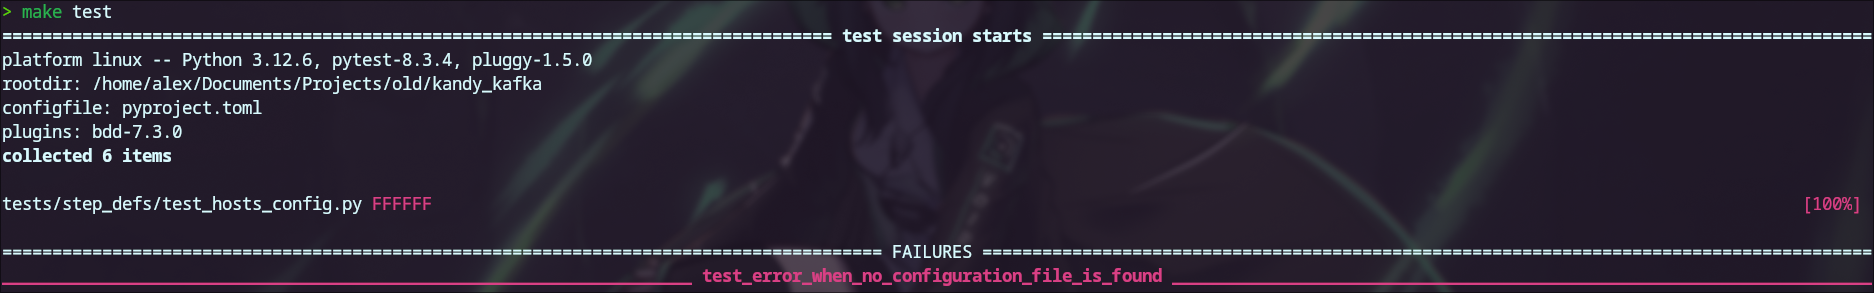
\includegraphics[width=0.95\textwidth]{imgs/FirstTestFailed.png}
  \end{center}
  \caption{Initial Test Failure}
\end{figure}

After confirming that the code doesn't work, I can start implementing features. The first test checks the system's behavior when the configuration file is missing:

\begin{code}
  \begin{minted}[]{Python}
# Non-existing configuration file scenario
@pytest.fixture
@given("Configuration file is not present")
def non_existing_config_file(tmp_path):
    return tmp_path / 'hosts.yaml'

@pytest.fixture
@when('system loads config')
def config():
    return Config()

@then('application should prompt user to create or specify a configuration file')
def check_prompt_to_create_config(config, non_existing_config_file):
    with pytest.raises(HostsFileNotFound):
        config.hosts_file = non_existing_config_file
        config.load_hosts('default')
  \end{minted}
\end{code}

Let’s break down what this test does:

\begin{itemize}
  \item \textbf{Given}: No configuration file is present. I provide a reference to a temporary auto-generated empty directory.
  \item \textbf{When}: I initialize the \texttt{Config} class
  \item \textbf{Then}: I plan to throw a custom exception, which will be caught and processed in the main function to display an error message in the terminal, it just makes design little bit cleaner, that printing error and exiting right after error. I will add a new method \texttt{load\_hosts} in the \texttt{Config} class to handle the configuration file and I'm gonna call it in my test (And probably in Bootstrap or entrypoint in actual code later).
\end{itemize}

The \texttt{Config} class now includes an additional field, \texttt{hosts\_file}, which will store the path to the configuration file. The default path is \texttt{"HOME\_DIRECTORY/.config/kandy/hosts.yaml"}. In the future, I'll need to refactor this to ensure platform compatibility (e.g., for Windows), but for this prototype, the current implementation is good enough. This field will be managed by the \texttt{load\_hosts} method, which accepts optional arguments for a custom configuration path and a cluster alias.

We’ll start with the simplest part, the exception. In the \texttt{exceptions.py} file, I create a new class that inherits from \texttt{Exception}:

\begin{code}
  \begin{minted}{Python}
  class HostsFileNotFound(Exception):
    pass
  \end{minted}
\end{code}

Now, I can raise this error and handle it elsewhere and thats it. Moving on to the \texttt{Config} module, I've revised how host and port fields are loaded from environment variables. Since the user can specify these via the command line, it makes sense to accept them as arguments during configuration initialization.

\begin{code}
  \begin{minted}{Python}
  import os
  from kandy_kafka import logger
  from pathlib import Path

  from kandy_kafka.exceptions import HostsFileHasWrongSyntax, HostsFileNotFound
  import yaml

  class Config:
      LOGGING_LEVEL: str

      KAFKA_HOST: str
      KAFKA_PORT: int

      def __init__(self, host=None, port=None) -> None:
          self.LOGGING_LEVEL = os.getenv("LOGGING_LEVEL", "INFO")
          logger.setup_logger(self.LOGGING_LEVEL)

          self.hosts_file = Path.home() / ".config" / "kandy" / "hosts.yaml"

          self.KAFKA_HOST = host
          self.KAFKA_PORT = port
  \end{minted}
\end{code}

The code uses Python's built-in \texttt{pathlib} library to determine the home directory, which simplifies future porting to Windows. \texttt{host} and \texttt{port} are passed as arguments but default to \texttt{None} since data can be sourced either from the command line or a configuration file. The \texttt{Config} class method will overwrite these values if the data is from a file.

Here’s the \texttt{load\_hosts} method:

\begin{code}
  \begin{minted}{Python}
    def load_hosts(self, clustername="default", config_file=None):
        if not self.hosts_file.exists():
            raise HostsFileNotFound(f"Hosts file {self.hosts_file} not found")

        if config_file:
            self.hosts_file = config_file
  \end{minted}
\end{code}

This method only checks for the file's existence and raises an error if it doesn’t exist, using the \texttt{pathlib} library's built-in functionality.

After implementing this, the code should pass the first test. Let’s run it using \texttt{make test}...

\begin{figure}[!htbp]
  \begin{center}
    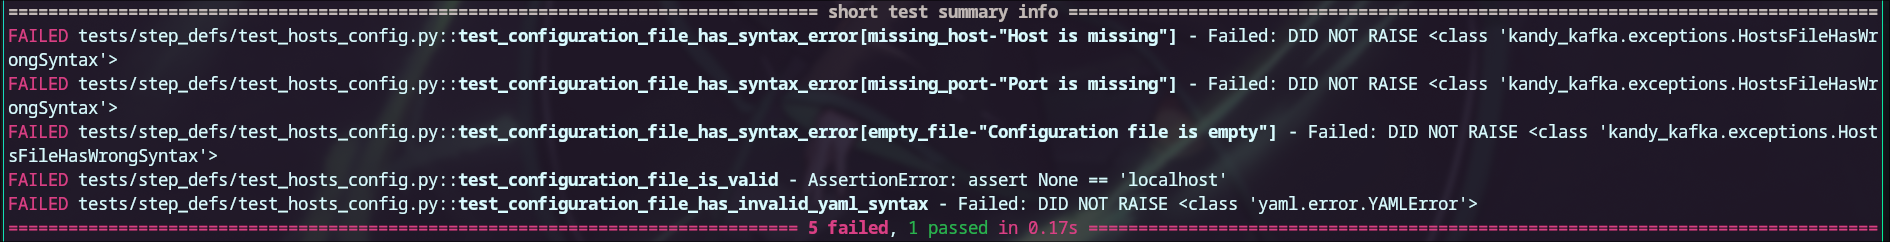
\includegraphics[width=0.95\textwidth]{imgs/BehaviourTestPassed.png}
  \end{center}
  \caption{}\label{fig:}
\end{figure}

After ensuring that the code works as intended, we proceed to the next test. This test verifies the system's behavior when the configuration file contains syntax errors. For this purpose, I utilized fixtures, which are pre-defined files, functions, and variables that create a testing environment. In this case, I used prepared configuration files. I divided the \textit{given} step into two parts: first, I create a file in the directory, and second, I write the contents of a specific fixture into that file. Since the test’s conditions are identical to the previous one (the \texttt{@when} step), \texttt{pytest} automatically reuses it, avoiding duplication.

Unfortunately, I could not resolve the issue of validating specific error messages in \texttt{stderr}. For now, the error message is simply printed during the test execution, but I left a \texttt{\# TODO} comment for future improvements.

\begin{code}
  \begin{minted}[samepage]{Python}
# Wrong syntax scenario
@pytest.fixture
@given("Configuration file is present")
def config_file(tmp_path):
    file = tmp_path / 'hosts.yaml'
    file.touch()
    return file

@pytest.fixture
@given(
    parsers.parse("Configuration file has {error_type} syntax error"),
    target_fixture='config_file_with_wrong_syntax'
)
def config_file_with_wrong_syntax(config_file, error_type):
    assert config_file.exists()
    config_fixture = Path("tests") / "fixtures" / "hosts" / f"wrong_syntax_{error_type}.yaml"
    config_file.write_text(config_fixture.read_text())

@then(parsers.parse("application should show {error}"))
def check_prompt_to_fix_syntax(config, error, config_file):
    print(error) # TODO check that actual error message is in the stderr (Or stdout)
    with pytest.raises(HostsFileHasWrongSyntax):
        config.load_hosts('default', config_file)
  \end{minted}
\end{code}

To handle this test, I introduced a new exception, \textbf{HostsFileHasWrongSyntax}, and updated the \texttt{load\_hosts} method in the \texttt{Config} class. This method now includes three checks:

\begin{itemize}
    \item \textbf{Is the file empty?}
    \item \textbf{Does the file contain the specified \texttt{clustername}?}
    \item \textbf{Are the \texttt{host} and \texttt{port} parameters correctly assigned?}
\end{itemize}

These checks cover all the cases I aimed to address. If new errors arise during manual testing, I can easily add corresponding tests and extend the code to handle them.

\begin{code}
  \begin{minted}[samepage]{Python}
def load_hosts(self, clustername="default", config_file=None):
    if not self.hosts_file.exists():
        raise HostsFileNotFound(f"Hosts file {self.hosts_file} not found")

    if config_file:
        self.hosts_file = config_file

    with open(self.hosts_file, "r") as file:
        hosts = yaml.safe_load(file)
        if hosts is None:
            raise HostsFileHasWrongSyntax(f"Hosts file {self.hosts_file} is empty")

        if clustername not in hosts:
            raise HostsFileHasWrongSyntax(
                f"Clustername {clustername} not found in {self.hosts_file}"
            )

        cluster = hosts[clustername]
        self.KAFKA_HOST = cluster.get("host")
        self.KAFKA_PORT = cluster.get("port")

    if not self.KAFKA_HOST or not self.KAFKA_PORT:
        raise HostsFileHasWrongSyntax(
            f"Host or port not found in {self.hosts_file}"
        )
  \end{minted}
  \caption{Updated load\_hosts Method}
\end{code}

After running the updated code...

\begin{figure}[htbp]
  \begin{center}
    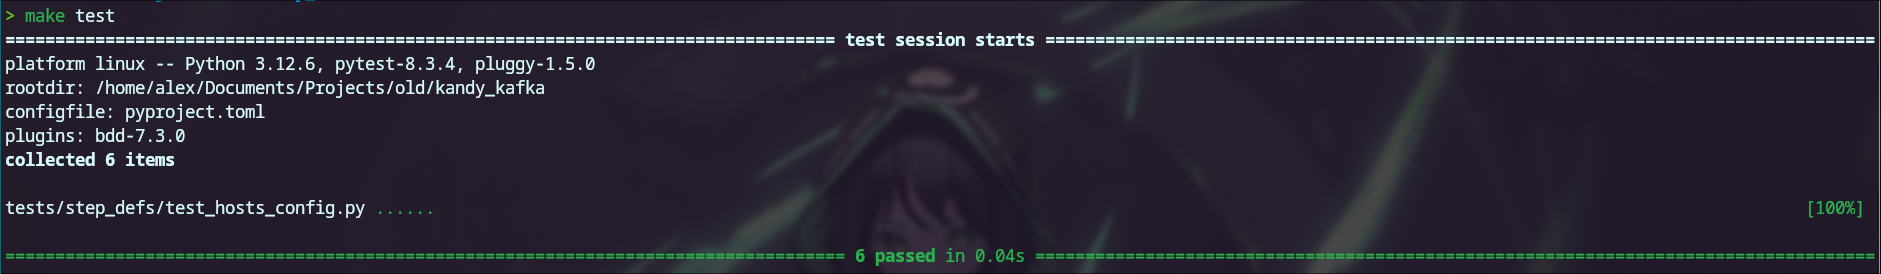
\includegraphics[width=0.95\textwidth]{imgs/FinalBehaviourTest.png}
  \end{center}
  \caption{Final Test Results}
\end{figure}

Surprisingly (or perhaps not so surprisingly), all tests pass. Why? Because the test we just implemented is not a single test—it verifies multiple scenarios using the same algorithm (as many scenarios as there are variations of the \texttt{error} field in the Gherkin script) and in our case it does mean that it covers 3 ot of 6 tests. The first one test still passes as I didn't change any functionality linked to it, and the remaining two tests validate the happy path(they check that everything works without errors when a valid configuration file is provided), and scenario when YAML syntax itself is incorrect. 

At this stage, no further changes are needed, as the code passes all tests. Ideally, I should begin refactoring. However, since the current codebase is relatively small and I am still drafting the prototype, clean code, while important, is not the highest priority at the moment.

As mentioned earlier, I wanted to add support not only for configuration files but also for CLI flags. This allows users to input parameters directly via the command line, for example:

\begin{code}
  \begin{minted}{bash}
  kandy --host "127.0.0.1" --port 8080
  \end{minted}
\end{code}

To implement flag (argument) support in Python, I utilized the built-in library \textbf{argparse}, which is specifically designed for this purpose.

Arguments clearly belong to the entry-point category, so I included them in the main file (`kandy.py`).

\begin{code}
  \begin{minted}{Python}
from kandy_kafka.bootstrap import Bootstrap
import argparse

class ConditionalAction(argparse.Action):
    def __call__(self, parser, namespace, values, option_string=None):
        if namespace.clustername:
            parser.error("clustername specified; --host and --port should not be used")
        setattr(namespace, self.dest, values)


def main():
    parser = argparse.ArgumentParser(description='Kandy Kafka')
    parser.add_argument("clustername", nargs='?', type=str, help='Cluster Name')
    parser.add_argument("--host", type=str, default=None, help='Host', action=ConditionalAction)
    parser.add_argument("--port", type=int, default=None, help='Port', action=ConditionalAction)

    args = parser.parse_args()

    if args.clustername and (args.host or args.port):
        parser.error("Clustername specified; --host and --port should not be used")
    if not args.clustername and (not args.host or not args.port):
        parser.error("If clustername is not specified, both --host and --port must be provided")

    Bootstrap()(clustername=args.clustername, host=args.host, port=args.port)

if __name__ == '__main__':
    main()
  \end{minted}
\end{code}

To prevent users from providing both `clustername` and `host`/`port` simultaneously, I implemented validation at the input level. While not a perfect solution, it is more than sufficient for an MVP project. Additionally, I passed `host`, `port`, and `clustername` as arguments to the `Bootstrap` class, which means it was time to modify the class to handle these new requirements.

The updated Bootstrap now accepts `**kwds` in the `\_\_call\_\_` method, extracting the necessary `port`, `host`, and `clustername`. I also added some logging; while not strictly necessary, it simplifies identifying where the application fails during startup, reducing debugging time and effort.

\begin{code}
  \begin{minted}[samepage]{Python}
from dataclasses import dataclass
import logging
from typing import Any
from kandy_kafka.adapters.kafka_adapter import KafkaAdapter
from kandy_kafka.config import Config


@dataclass
class Bootstraped:
    config: Config
    kafka_adapter: KafkaAdapter


class Bootstrap:
    bootstraped: Bootstraped

    def __call__(self, *args: Any, **kwds: Any) -> Bootstraped:
        logging.info("ATTEMPTING TO BOOTSTRAP - loading config")
        config = Config(kwds["host"], kwds["port"])

        if kwds["clustername"]:
            config.load_hosts(kwds["clustername"])

        logging.info("ATTEMPTING TO BOOTSTRAP - creating KafkaAdapter")
        kafka_adapter = KafkaAdapter(config.KAFKA_HOST, config.KAFKA_PORT)

        Bootstrap.bootstraped = Bootstraped(
            config=config,
            kafka_adapter=kafka_adapter,
        )

        logging.info("BOOTSTRAPING Completed")

        return Bootstrap.bootstraped
  \end{minted}
\end{code}

After adding this code we run tests again, just to check that everything works as it should and now we can start application from a CLI, so first step is done

\subsection{Connecting to Kafka}

The next step involves working with topics, which means integration with Kafka. In most companies, Kafka is hosted in the cloud on dedicated servers, but I don’t have that luxury, and during development, it’s not always convenient to have something running on a remote server instead of locally. Therefore, I will test it in an environment composed of Docker containers. I already mentioned Docker in the analysis section, but I think it won't hurt to repeat it. Docker is a tool for containerizing services. Simply put, it allows you to run any service wherever it can run itself, which is extremely convenient. Additionally, I can externally and internally manipulate containers to simulate load and various conditions that might be challenging to test on a real server, which is why I use Docker.

Setting up containers is simple: find an image on the official website, copy its name, add it to a configuration file, and voilà, the service runs like new. However, as I mentioned, Docker allows very fine-tuned control of the environment and offers many optional yet interesting parameters. Now, I'll show the resulting configuration and explain how it works:

\begin{code}
  \begin{minted}[fontsize=\small]{YAML}
    version: '3.8'

services:
  zookeeper:
      image: "confluentinc/cp-zookeeper"
      ports:
        - 32181:32181
      environment:
        - ZOOKEEPER_CLIENT_PORT=32181

  kafka:
      image: confluentinc/cp-kafka
      ports:
        - 9092:9092
        - 29092:29092
      healthcheck:
        test: nc -z localhost 9092 || exit -1
        start_period: 15s
        interval: 5s
        timeout: 10s
        retries: 10
      depends_on:
        - zookeeper
      environment:
        - KAFKA_BROKER_ID=1
        - KAFKA_ZOOKEEPER_CONNECT=zookeeper:32181
        - KAFKA_ADVERTISED_LISTENERS=PLAINTEXT://kafka:9092, PLAINTEXT_HOST://localhost:29092
        - KAFKA_LISTENER_SECURITY_PROTOCOL_MAP=PLAINTEXT:PLAINTEXT, PLAINTEXT_HOST:PLAINTEXT
        - KAFKA_INTER_BROKER_LISTENER_NAME=PLAINTEXT
        - KAFKA_OFFSETS_TOPIC_REPLICATION_FACTOR=1
    
  init-kafka:
    image: confluentinc/cp-kafka
    depends_on:
      kafka:
        condition: service_healthy
    entrypoint: ["/bin/sh", "-c"]
    command: |
      "
      # blocks until kafka is reachable
      kafka-topics --bootstrap-server kafka:9092 --list
      echo -e 'Creating kafka topics'
      kafka-topics --bootstrap-server kafka:9092 --create --if-not-exists --topic test --replication-factor 1 --partitions 1
      kafka-topics --bootstrap-server kafka:9092 --create --if-not-exists --topic test2 --replication-factor 1 --partitions 1
      echo -e 'Successfully created the following topics:'
      kafka-topics --bootstrap-server kafka:9092 --list
      "
  \end{minted}
  \caption{Docker Compose configuration for Kafka}
\end{code}

So, what's happening here? I am launching Kafka and forwarding ports from the container to the host machine. This way, the service can be accessed via my computer's address (in my case, simply `localhost`) on ports 9092 and 29092. Then come the environment variables, which are essential for Kafka to function. However, there are several parameters, such as encryption type, login credentials, and a few Kafka-specific settings that I probably won’t need to use.

As I described in section~\ref{Kafka_architecture}, Kafka currently depends on another service called Zookeeper, so I had to set it up as well and configure interactions between the services. I added a third service as a testing platform—more precisely, a platform with tests. This service will populate Kafka with test data. It is linked to the main system and monitors its "health" at the beginning, ensuring it won't push data into an uninitialized container.

At the moment, the `init-kafka` (as I will call the testing platform) service simply creates two empty topics. I might switch to Python fixtures in the future, but for now, this approach seems more reasonable. As for Python, specifically the tests, they turned out to be relatively simple. In the future, I plan to add checks for messages and additional tests.

\begin{code}
  \begin{minted}[fontsize=\small]{bash}
echo -e 'Creating Kafka topics'
for i in {1..3}; do
  kafka-topics --bootstrap-server kafka:9092 --create --if-not-exists --topic "test$i" --replication-factor 1 --partitions 1
done

echo -e 'Kafka topics:'
kafka-topics --bootstrap-server kafka:9092 --list

echo -e 'Filling test1 topic with 10 messages'
for i in {1..10}; do
  echo "Message$i" | kafka-console-producer --bootstrap-server kafka:9092 --topic test1
done

echo "askdl" >> /tmp/healthy

tail -f /dev/null

  \end{minted}
  \caption{Population script}
\end{code}

After some consideration, I decided to refine my approach: instead of configuring Kafka directly in `docker-compose`, I will handle it through a separate script. This script will be invoked from the `Dockerfile`, which will then be used in `docker-compose`. 

\begin{code}
  \begin{minted}{YAML}
FROM confluentinc/cp-kafka:latest

WORKDIR /app

COPY tests/kafka_setup.sh ./create_and_fill_topics.sh

USER root
RUN chmod +x ./create_and_fill_topics.sh

CMD ["/bin/bash", "-c", "./create_and_fill_topics.sh"]

  \end{minted}
\end{code}

While this might initially sound complex, in reality, this approach simplifies the process. By separating logic into a script, I can easily manage operations. For instance, instead of making 30 individual calls to "add a message," I can write a loop and execute it efficiently. This not only improves flexibility but also makes the configuration and maintenance process significantly smoother.

\subsubsection{Writing Integration Tests}

\begin{code}
  \begin{minted}[samepage]{Python}
  import pytest
from kandy_kafka.adapters.kafka_adapter import KafkaAdapter


@pytest.fixture
def kafka_adapter(server):
    """Instantiate a KafkaAdapter object and return it as a fixture"""
    adapter = KafkaAdapter(server.HOST, server.PORT)
    yield adapter


def test_should_return_topic_list(kafka_adapter):
    topics = kafka_adapter.get_topics()
    assert isinstance(topics, list)
    assert all(topic in topics for topic in ["test1", "test2", "test3"])
  \end{minted}
\end{code}

I created a small fixture that returns an adapter and performs a teardown after the test either passes or fails. Additionally, I wrote a test that verifies the amount and names of topics match the actual state. In the future, message verification checks will be added here.

After running the test and confirming that it fails as expected, I proceeded to implement the code. The structure of the adapter was predefined by me on previous step; I just needed to fill it with functionality. After reading the `confluent\_kafka` documentation, I found several ways to connect to Kafka and examples of how to interact with the system. Based on these examples, I wrote a method to retrieve topics. At this stage, it consists of just a few lines of code that return topic names as strings. This is sufficient for this test but later, I will refactor the method to return data in the form of an internal model (a `dataclass` called `Topic`), which will include not only the name but also partitions, load, and other necessary details.

\newpage
\begin{code}
  \begin{minted}{Python}
from abc import ABC, abstractmethod
from confluent_kafka.admin import AdminClient
from confluent_kafka import Consumer, KafkaException, TopicPartition
from datetime import datetime, timedelta

from typing import List

import logging 

class AbstractKafkaClusterAdapter(ABC):
    @abstractmethod
    def get_topics(self) -> List[str]:
        raise NotImplementedError

    @abstractmethod
    def get_messages(self, topic: str) -> List[str]:
        raise NotImplementedError

class KafkaAdapter(AbstractKafkaClusterAdapter):
    def __init__(self, host: str, port: int):
        self.admin_client = AdminClient({
            "bootstrap.servers": f"{host}:{port}"
        })
    
    def get_topics(self) -> List[str]:
        topics = self.admin_client.list_topics(timeout=10).topics
        return list(topics)
  \end{minted}
\end{code}

The test passes, and the topic names are returned correctly. However, there is a small issue with testing.

\begin{figure}[htbp]
  \begin{center}
    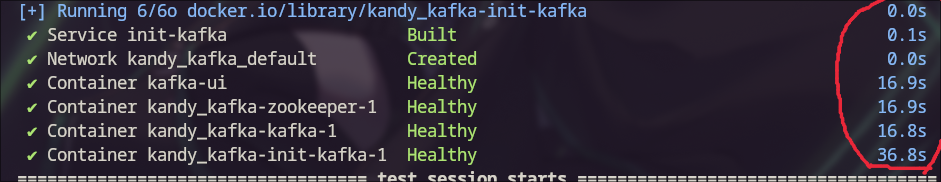
\includegraphics[width=0.95\textwidth]{imgs/TestingTimings.png}
  \end{center}
  \caption{Testing timings issue during integration tests}\label{fig:}
\end{figure}

The method I chose to populate Kafka with data works extremely slowly due to the nature of the utility. While this does not directly impact the product, it affects the development process. I spend about a minute just to test the integration. When introducing new features, tests need to be run frequently, and as a result, instead of coding, I end up waiting for everything to build and test.

In the near future, I need to find a new way to test this functionality. For now, I have excluded integration tests from the main pipeline and will run them manually only when changes are made to the adapter.

\subsection{GUI: Topics}

Kafka integration is set up, data retrieval works, and configuration initialization is complete. Now, it's time for the most important part of the whole TUI — the actual UI. I started with `urwid` and created several basic classes that describe fundamental entities such as panels, tables, search boxes, and more. I then arranged these components on the screen, almost following the design. This process was challenging and time-consuming due to the outdated documentation for `urwid`, but I eventually achieved the following result:

\begin{code}
  \begin{minted}{Python}
from typing import List
from kandy_kafka.models import Topic

import urwid
import re

import logging

class TopicsView:
    def __init__(self, controler):
        self.controler = controler
        self.elements = {
            "topics_names": TopicsList(self),
            "topic_data": TopicDataPanel()
            }
        self.columns = urwid.Columns([
            ('weight', 1, self.elements["topics_names"].show()),
            ('weight', 1.5, self.elements["topic_data"].show())
        ], dividechars=1)

    def update_topics_names(self, topics_names: List[str]):
        self.elements["topics_names"].update_topics(topics_names)
        self.show()

    def get_topic(self, topic_name: str):
        return self.controler.get_topic(topic_name)
    
    def show(self):
        self.columns.contents[0] = (self.elements["topics_names"].show(), self.columns.options())
        self.controler.loop.draw_screen()


class TopicsList:
    def __init__(self, parent_view) -> None:
        self.parent_view = parent_view
        
        # Topics
        self.topics_names = []
        self.topics_list = urwid.SimpleFocusListWalker([])
        
        # Search Field
        self.search_field = urwid.Edit('Search: ')
        urwid.connect_signal(self.search_field, 'change', self.update_on_search)
        self.search_text = ''
        
        # UI
        self.listbox = self.FocusChangeListBox(self.topics_list, self.select_topic)
        self.layout = urwid.LineBox(urwid.Pile([self.listbox]), tlcorner='╭', trcorner='╮', blcorner='╰', brcorner='╯')
        self.last_focus = None
        self.layout = urwid.Pile([('pack', urwid.LineBox(self.search_field, tlcorner='╭', trcorner='╮', blcorner='╰', brcorner='╯')), self.layout])

    class FocusChangeListBox(urwid.ListBox):
        def __init__(self, body, on_focus_changed):
            super().__init__(body)
            self.on_focus_changed = on_focus_changed

        def keypress(self, size, key):
            focus_widget, _ = self.get_focus()
            key = super().keypress(size, key)
            if self.get_focus() != (focus_widget, _):
                self.on_focus_changed(None, None)
            return key
        
    def filter_topics(self):
        search_text = self.search_text
        logging.info(f"Filtering topics with search text: {search_text}")
        if search_text:
            pattern = re.compile(search_text, re.IGNORECASE)
        else:
            pattern = re.compile('.*')
        
        self.topics_list.clear()
        for topic_name in self.topics_names:
            if pattern.search(topic_name):
                selectable_item = urwid.SelectableIcon(topic_name, 100)
                self.topics_list.append(urwid.AttrMap(selectable_item, None, focus_map='focused'))

    def show(self):
        self.filter_topics()
        if self.last_focus is not None and self.last_focus < len(self.topics_list):
            self.topics_list.set_focus(self.last_focus)
        return self.layout
    
    def update_on_search(self, edit, new_edit_text):
        logging.info(f"Search text changed to: {new_edit_text}")
        self.search_text = new_edit_text
        self.parent_view.show()
            
    def update_topics(self, topics_names: List[str] = None):
        if topics_names is not None:
            self.topics_names = topics_names

    def get_selected_topic(self):
        if self.last_focus is not None and self.last_focus < len(self.topics_list):
            return self.topics_list[self.last_focus].get_text()[0]

    def select_topic(self, button, user_data):
        _, self.last_focus = self.topics_list.get_focus()


class TopicDataPanel:
    def __init__(self) -> None:
        self.topic_data = urwid.Text('')
        self.rounded_layout = urwid.LineBox(self.topic_data, tlcorner='╭', trcorner='╮', blcorner='╰', brcorner='╯')

    def show(self):
        return urwid.AttrMap(self.rounded_layout, "colored")

    def update(self, topic: Topic):
        data = {"name": topic.name,
                "is_internal": topic.is_internal,
                "Number of partitions": len(topic.partitions),
                "Partitions": [partition.id for partition in topic.partitions]}
        final_data = '\n'.join([f'{key}: {value}' for key, value in data.items()])
        self.topic_data.set_text(final_data)

  \end{minted}
\end{code}

Before integrating the UI into the main system, I tested it in a separate local window. I hardcoded a list of topics and observed how the UI responded to various actions. Overall, everything works well except for one issue.

\newpage
\begin{figure}[htbp]
  \begin{center}
    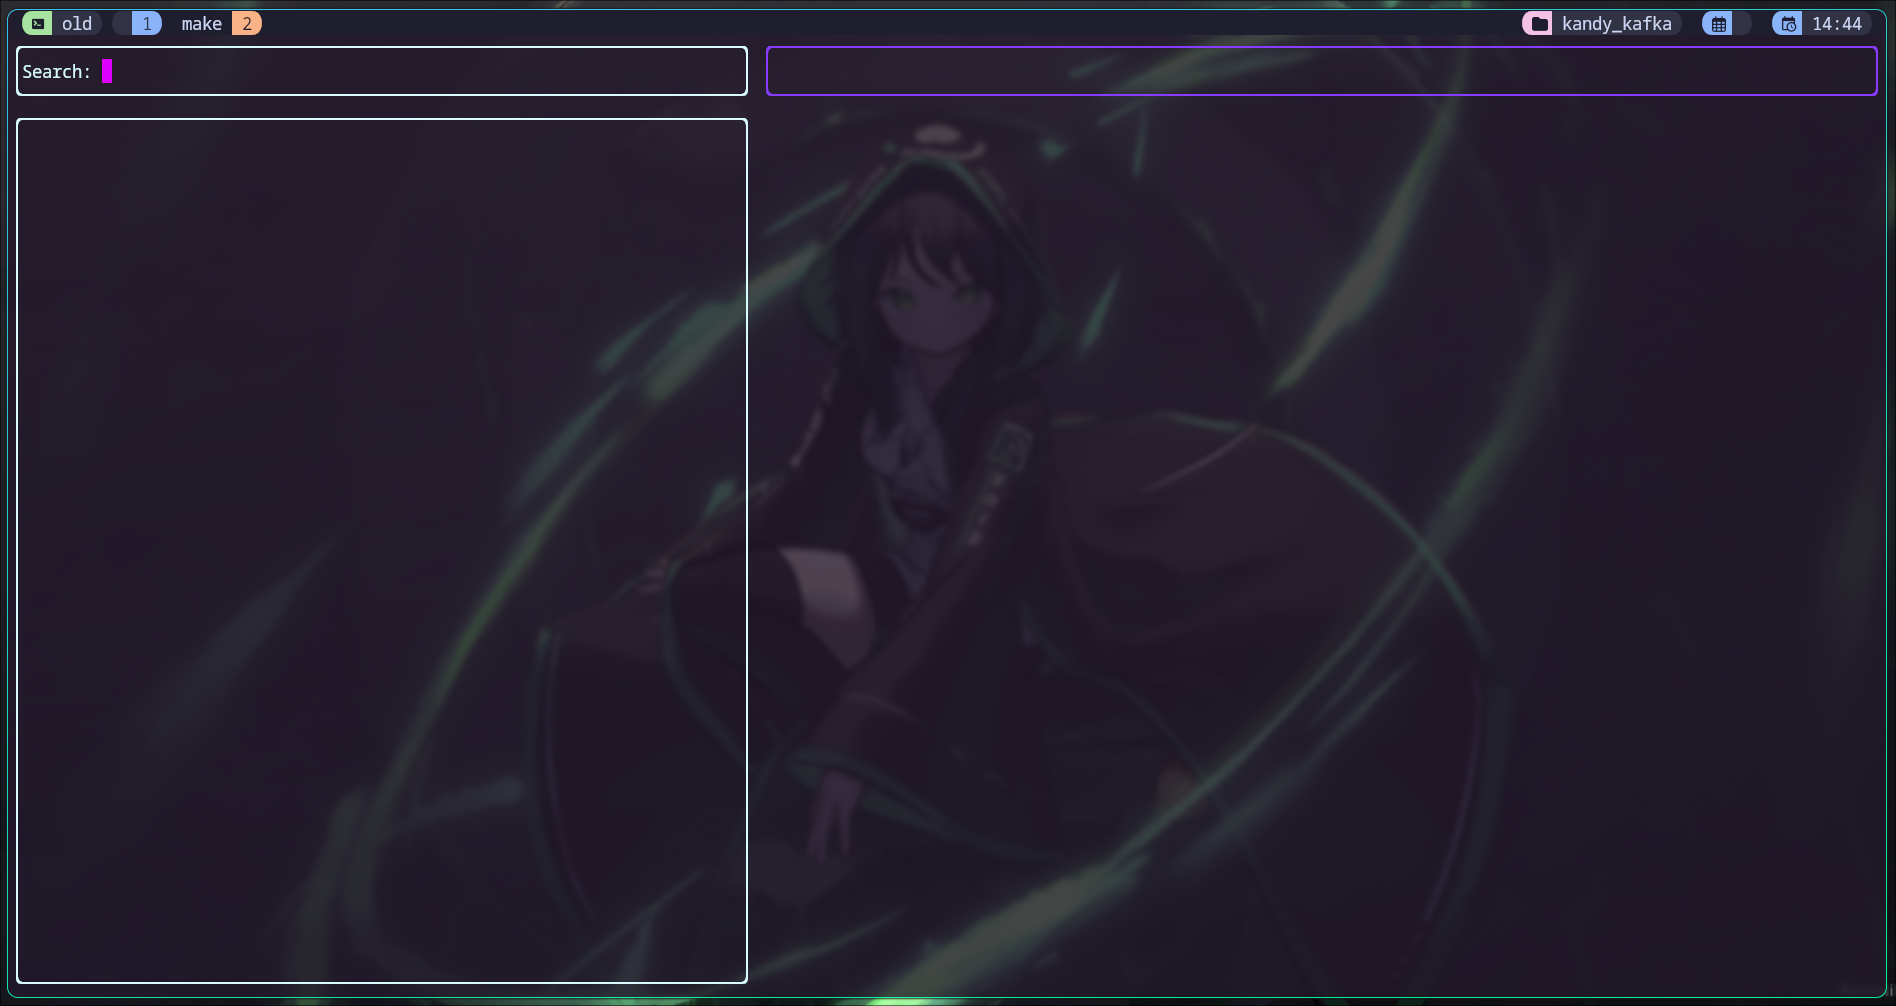
\includegraphics[width=0.95\textwidth]{imgs/UIFirstScreen.png}
  \end{center}
  \caption{}\label{fig:}
\end{figure}

I was unable to configure the display as a table instead of a list because `urwid` does not natively support such functionality. While trying to solve this issue, I discovered a library called `panwid` that includes several widgets, but it failed to work in my environment due to version conflicts with the `pydantic` library. Since `pydantic` is used both in my project and in `panwid`, I had to abandon `panwid`. Eventually, I also decided to move away from `urwid` entirely and switched to using `textual`, as it seemed simpler and more suitable for my needs.

Below is an example of the code I wrote to test the table functionality:

\begin{code}
  \begin{minted}{Python}
import urwid

import random
import uuid
from typing import List

from panwid.datatable import DataTable, DataTableColumn, DataTableDivider


class RoundedBox(urwid.LineBox):
    def __init__(self, body):
        super().__init__(body, tlcorner="╭", trcorner="╮", blcorner="╰", brcorner="╯")


class HorizontalMenu(urwid.Padding):
    def __init__(self):
        menu = urwid.Columns(
            [
                urwid.SelectableIcon("Consumers"),
                urwid.SelectableIcon("Topics"),
                urwid.SelectableIcon("Brokers"),
                urwid.SelectableIcon("Exit"),
            ],
        )
        super().__init__(menu, left=2, right=100, min_width=100)


class SearchBar(RoundedBox):
    def __init__(self):
        super().__init__(urwid.Edit("Search: "))


class TopicsDataTable(RoundedBox):
    def __init__(self, topics: List):
        columns = [
            DataTableColumn(
                "topic",
                "Topic",
                width=("weight", 2),
                align="center",
                format_fn=lambda x: x.upper(),
            ),
            DataTableDivider("\N{BOX DRAWINGS DOUBLE VERTICAL}"),
            DataTableColumn(
                "partitions",
                "Partitions",
                align="center",
                width=(13),
            ),
            DataTableDivider("\N{BOX DRAWINGS DOUBLE VERTICAL}"),
            DataTableColumn(
                "brokers",
                "Brokers",
                align="center",
            ),
            DataTableDivider("\N{BOX DRAWINGS DOUBLE VERTICAL}"),
            DataTableColumn(
                "size",
                "Size",
                align="center",
            ),
        ]
        data = [
            dict(topic=topic, partitions=partitions, brokers=brokers, size=size)
            for topic, partitions, brokers, size in topics
        ]
        table = DataTable(
            columns=columns,
            data=data,
            with_scrollbar=True,
            sort_refocus=True,
            cell_selection=True,
        )
        super().__init__(urwid.Frame(table))


class TopicsList(urwid.Pile):
    def __init__(self, topics: List):
        super().__init__([("pack", SearchBar()), TopicsDataTable(topics)])


class TopicDetail(RoundedBox):
    def __init__(self, topic: str):
        body = urwid.Filler(urwid.Text(topic), valign="top")
        super().__init__(body)


class TopicsView(urwid.Columns):
    def __init__(self, topics: List):
        super().__init__([TopicsList(topics), TopicDetail("Topic detatils")])


class Main:
    def __init__(self, topics: List):
        palette = [
            ("table_row_body", "", ""),
            ("table_row_body focused", "white", "black"),
            ("table_row_body column_focused", "", "black"),
            ("table_row_body highlight", "", ""),
            ("table_row_body highlight focused", "", "black"),
            ("table_row_body highlight column_focused", "", "black"),
            ("table_row_header", "", ""),
            ("table_row_header focused", "", ""),
            ("table_row_header column_focused", "", "black"),
            ("table_row_header highlight", "", "yellow"),
            ("table_row_header highlight focused", "", "yellow"),
            ("table_row_header highlight column_focused", "", "yellow"),
            ("table_row_footer", "", "white"),
            ("table_row_footer focused", "", "dark gray"),
            ("table_row_footer column_focused", "", "black"),
            ("table_row_footer highlight", "", "yellow"),
            ("table_row_footer highlight focused", "", "yellow"),
            ("table_row_footer highlight column_focused", "", "yellow"),
        ]
        layout = urwid.Frame(body=TopicsView(topics), header=HorizontalMenu())
        self.loop = urwid.MainLoop(layout, palette=palette)

    def run(self):
        self.loop.run()


if __name__ == "__main__":
    # random data
    n = 100
    topics = [
        (
            uuid.uuid4().hex,
            random.randint(1, 10),
            random.randint(1, 10),
            random.randint(1, 10),
        )
        for _ in range(n)
    ]
    Main(topics).run()
  \end{minted}
\end{code}

\newpage
\subsection{Switching to Textual}

I found `textual` appealing due to its well-structured documentation and development approach. It allowed me to focus on high-level functionality rather than dealing with "low-level" details while working with widgets. With `textual`, I can simply combine widgets and use event-driven programming to handle interactions in a modular and organized way, which is extremely convenient.

After experimenting with `textual`, I decided to deviate slightly from the strict view-controller system and give the view layer a bit more freedom. In a real product, I would adhere to the MVC architecture, as it is harder to implement initially but pays off in the long run by simplifying debugging and review processes. However, for this coursework MVP, my priority is to have functional, readable code that works well, even if it’s not perfectly architected.

The rewrite from `urwid` to `textual` resulted in significantly cleaner and more organized code. Additionally, I’ve started adding comments to improve clarity.

\begin{code}
  \begin{minted}{Python}
# kandy_kafka/gui/views/topics.py
  
from textual.widgets import DataTable, Header, Footer
from textual.containers import Container
from textual.app import ComposeResult


class TopicsView(Container):
    """View to display topics in a table."""

    def __init__(self):
        super().__init__()
        self.table = DataTable()

    def build_table(self, topics: list[str]):
        """Build the DataTable widget to display the topics."""
        self.table.clear()
        self.table.add_column("Topics")
        for topic in topics:
            self.table.add_row(topic)

    def compose(self) -> ComposeResult:
        """Compose the view with the table."""
        yield Header()
        yield self.table
        yield Footer()

  \end{minted}
\end{code}

`textual` comes with a built-in `DataTable` component, which simplified the implementation of tables immensely. It also offers a variety of customizable and well-documented widgets, such as `Header` and `Footer`. These are features I had to implement manually in `urwid`, often without proper documentation, by reading and modifying the library’s source code to fix bugs. In `textual`, these components are beautifully designed and ready to use, making development faster and smoother.

Next, I decided to integrate the UI with the rest of the code and rewrote the controller.

\begin{code}
  \begin{minted}{Python}
# kandy_kafka/gui/controller.py

# The code block below is needed to avoid a cyclic import error, while using Bootstrap class for type-hinting
from __future__ import annotations
from typing import TYPE_CHECKING

if TYPE_CHECKING:
    from kandy_kafka.bootstrap import Bootstraped

from textual.app import App, ComposeResult
from kandy_kafka.gui.views import TopicsView
from typing import TYPE_CHECKING

if TYPE_CHECKING:
    from kandy_kafka.bootstrap import Bootstraped


class Controller(App):
    """Main application controller"""

    BINDINGS = [("f", "fetch", "fetch")]
    CSS_PATH = "app.tcss"  # Textual CSS file for styling

    def __init__(self, bootstraped: Bootstraped):
        super().__init__()
        self.bootstrapped = bootstraped
        self.kafka_adapter = self.bootstrapped.kafka_adapter
        self.view = TopicsView()  # Instantiate the TopicsView from views.py

    async def reload_topics(self):
        """
        Reload the topics by pulling them from the KafkaModel and updating the TopicsView.
        """
        topics = self.kafka_adapter.get_topics()  # Fetch topics from Kafka
        self.view.build_table(topics)  # Update the table in the view

    async def action_fetch(self) -> None:
        """Handle the message to reload topics."""
        await self.reload_topics()

    def compose(self) -> ComposeResult:
        """Compose the app layout."""
        yield self.view  # Adds the TopicsView (table)

  \end{minted}
\end{code}

`textual` comes with several useful features, such as key bindings and CSS-like styles for applications. Although these are empty for now, I plan to explore them in the future to create a more visually appealing interface.

The controller currently has one primary function, `reload\_topics`, which retrieves data from Kafka and displays it in the table format (for now, just a single column with the topic name). The `action\_fetch` function is triggered by the specified key binding, which in this case is `f`. The bindings are defined in the `BINDINGS` variable: `BINDINGS = [("f", "fetch", "fetch")]`. In the future, I could add usability features for configuring shortcut keys.

In the bootstrap, I added just a few lines to import and initialize the controller:

\begin{code}
  \begin{minted}{Python}
      from kandy_kafka.gui.controller import Controller
      
      controller = Controller(Bootstrap.bootstraped)
      controller.run()
  \end{minted}
\end{code}

I also started experimenting with message retrieval, but I’ll discuss that later since I encountered some challenges there. These were all the changes made at this point.

\begin{figure}[htbp]
  \begin{center}
    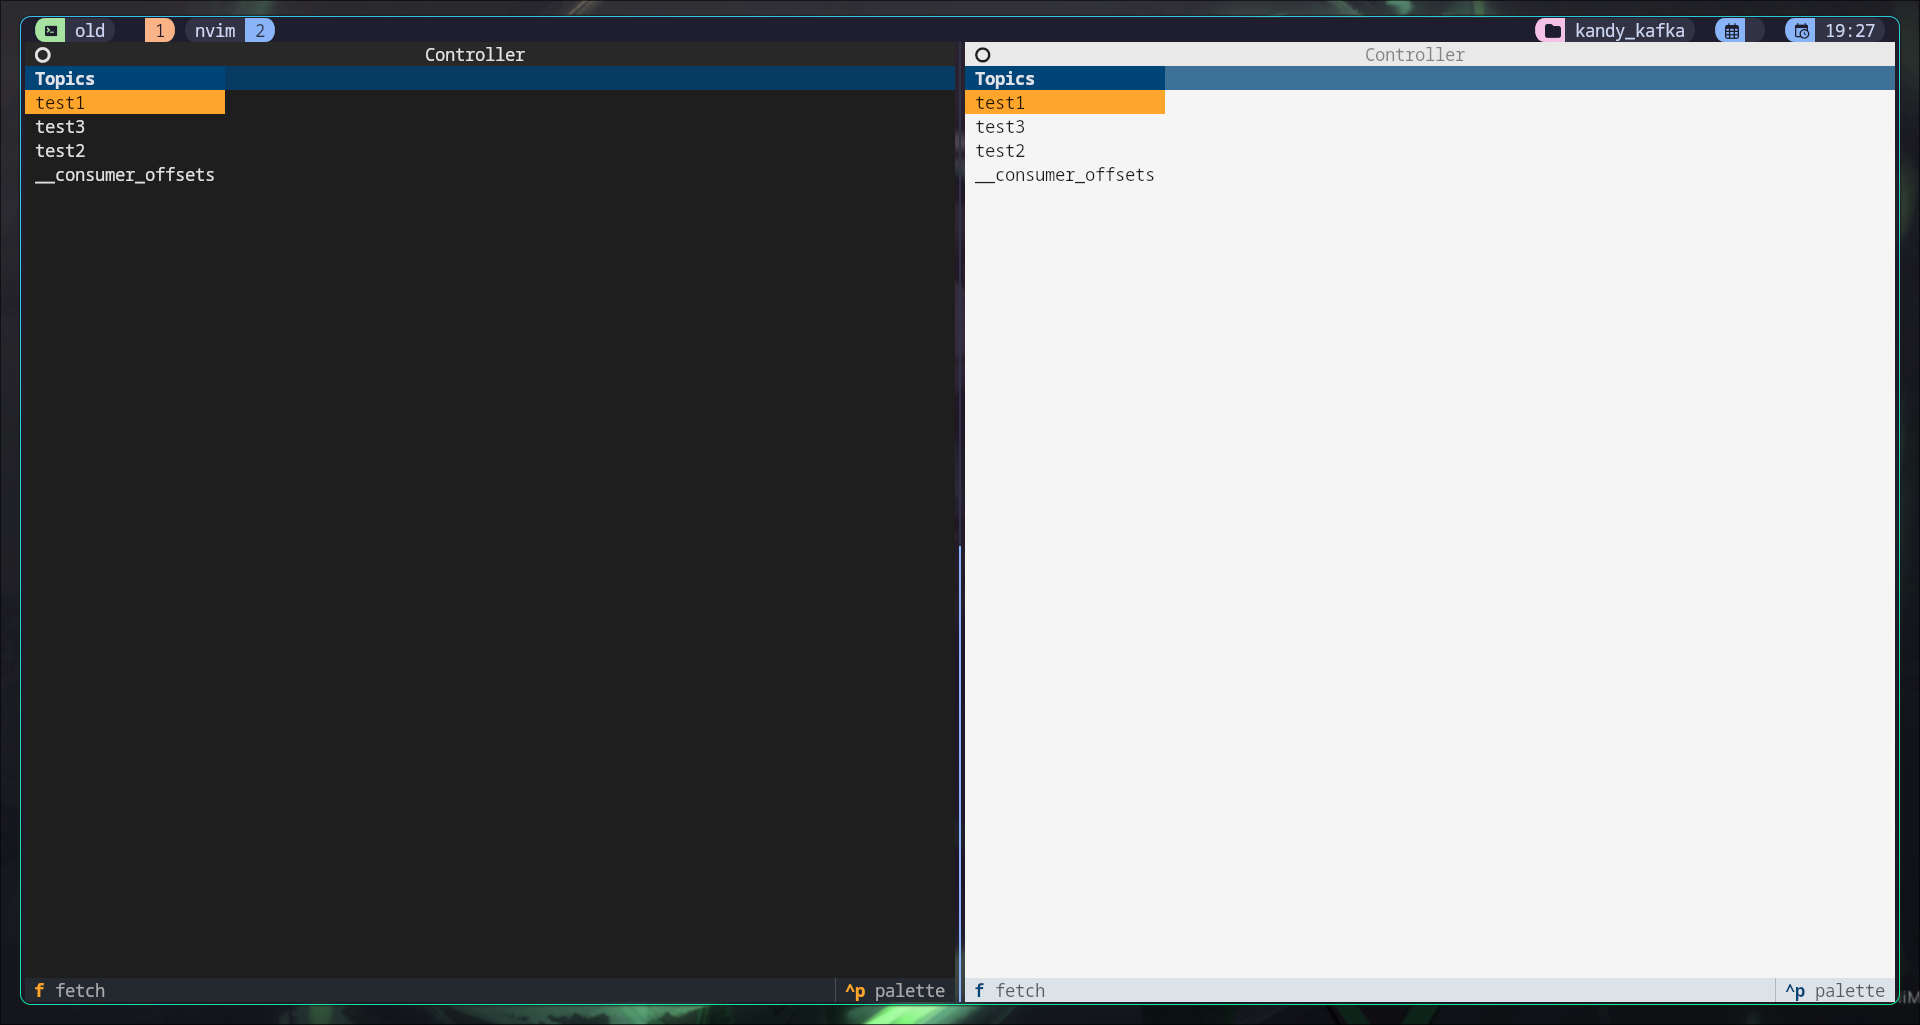
\includegraphics[width=0.95\textwidth]{imgs/TextualFirstScreen.png}
  \end{center}
  \caption{}\label{fig:}
\end{figure}

When the utility launches, it displays a window like the one shown above. Pressing the `f` key fetches topics from Kafka. At this stage, there are no filters implemented, so both system and user topics are displayed. However, I encountered a critical bug, which I haven’t fixed yet and plan to address later.

The bug occurs when the Kafka server is not running (or unavailable on the host). Instead of raising an `Exception`, `confluent\_kafka` logs errors directly to stdout and repeatedly attempts to reconnect. During this process, the application becomes unresponsive to user input, including the `Ctrl-C` command (a common way to stop applications in Linux), effectively locking the terminal.

\newpage
\begin{figure}[htbp]
  \begin{center}
    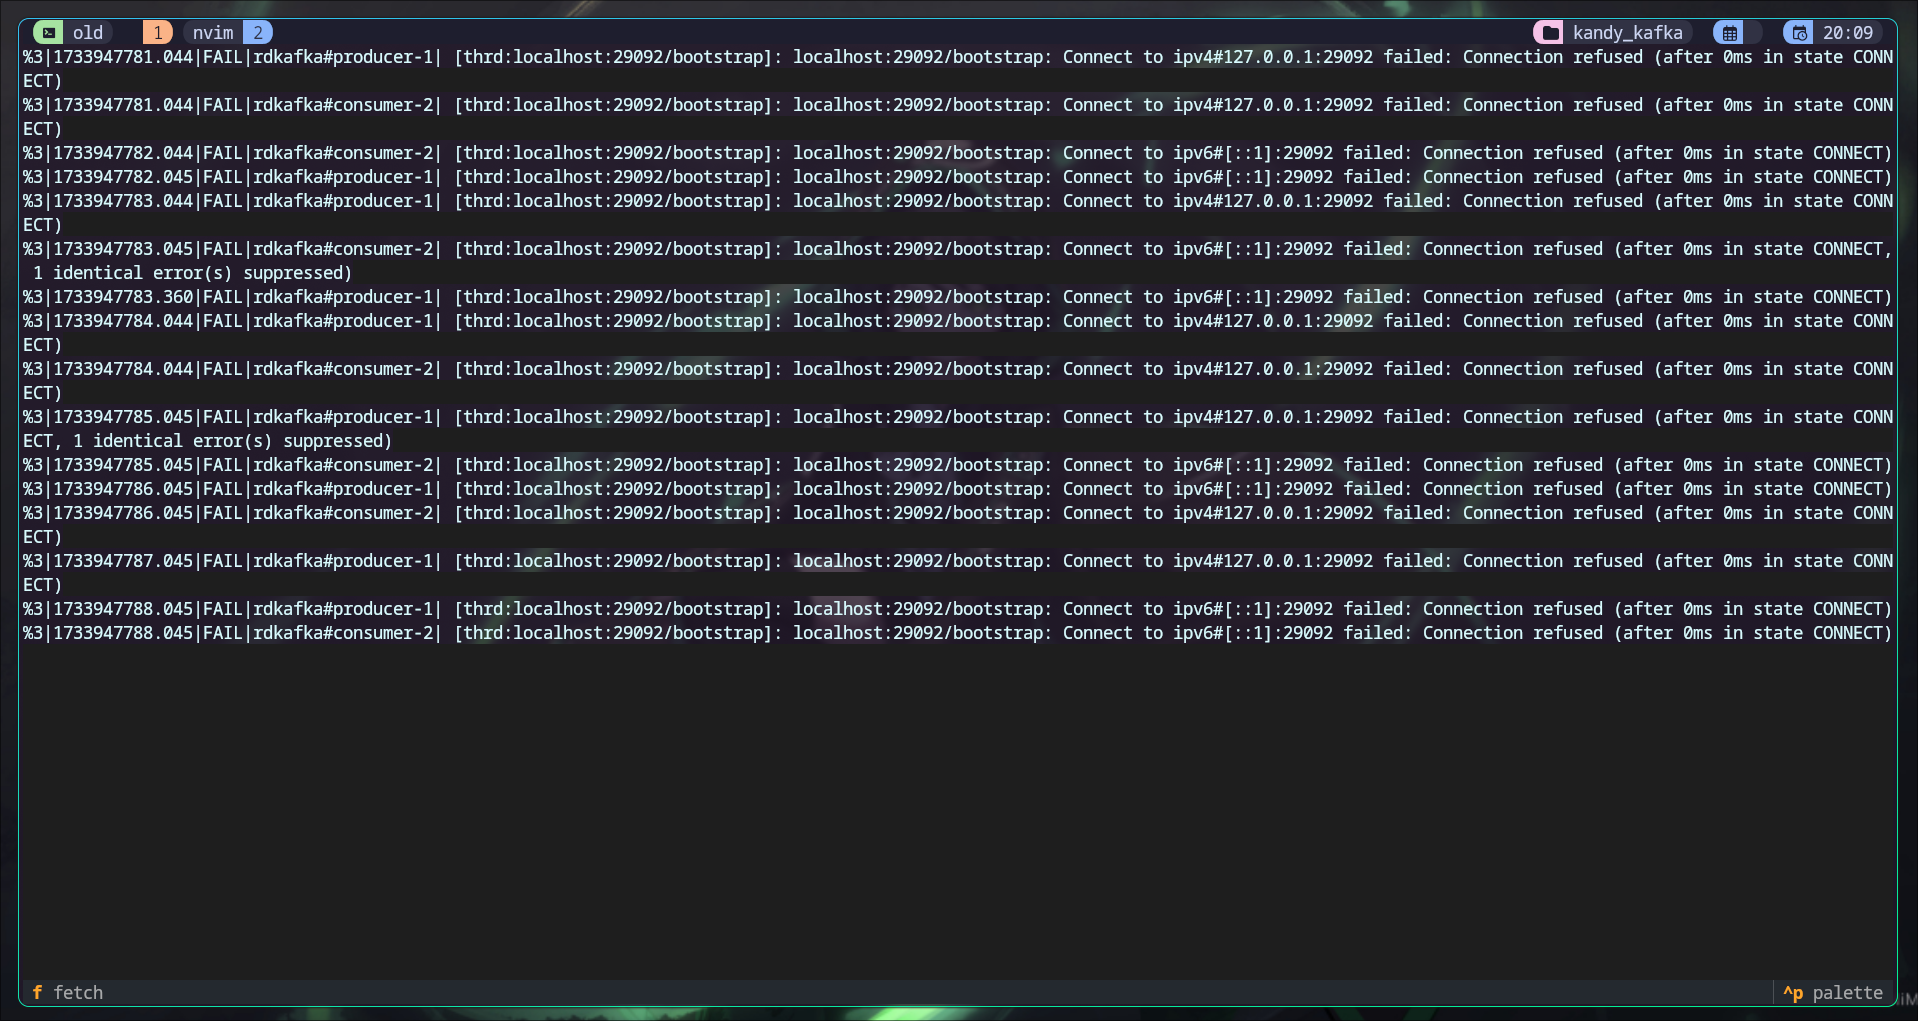
\includegraphics[width=0.95\textwidth]{imgs/BrokerConnectionError.png}
  \end{center}
  \caption{}\label{fig:}
\end{figure}

While this issue might not be critical for an MVP, it is unacceptable for a production-grade application. I think the solution would involve creating a wrapper that pings the server before attempting a connection, ensuring Kafka is available on the specified port. Ideally, the application should fail gracefully and provide an immediate, clear error message. Unfortunately, I couldn’t find any references in the `confluent\_kafka` documentation on how to implement such behavior ot at least dissabling this errors in their library.

\subsection{Finish Line}

I haven’t outlined every iteration that led to the final result, but in this section, I’ve highlighted and explained several major bugs and general challenges I encountered during development, as well as the thought process behind resolving them.

Initially, I anticipated that implementing topic search functionality would be problematic and delayed working on it for a long time. However, it turned out that regular expressions handled the task exceptionally well, and `textual` provided an excellent interface for working with data tables. Ultimately, the only remaining steps were to write a suitable regex and handle sorting method combinations, which proved to be less complex than expected.

\begin{code}
  \begin{minted}{Python}
    def compose(self) -> ComposeResult:
        """Compose the view with the table."""
        yield Horizontal(
            Vertical(
                ListView(
                    ListItem(Label("Brokers")),
                    ListItem(Label("Topics")),
                    ListItem(Label("Consumers")),
                ),
                id="navigation-pane",
            ),
            Vertical(
                Input(placeholder="Search Topics...", id="search-field"),
                self.table,
                id="center-pane",
            ),
        )

    current_sorts: set = set()

    def sort_reverse(self, sort_type: str):
        """Determine if `sort_type` is ascending or descending."""
        reverse = sort_type in self.current_sorts
        if reverse:
            self.current_sorts.remove(sort_type)
        else:
            self.current_sorts.add(sort_type)
        return reverse

    def action_sort_by_size(self) -> None:
        table = self.query_one(DataTable)
        table.sort(
            "Size",
            key=lambda x: x,
            reverse=self.sort_reverse("Size"),
        )

    def action_sort_by_partitions(self) -> None:
        table = self.query_one(DataTable)
        table.sort(
            "Partitions", key=lambda x: int(x), reverse=self.sort_reverse("Partitions")
        )

    async def on_input_changed(self, event):
        """Called whenever the input in the search field changes."""
        search_query = event.value.strip()

        if search_query == "":
            # If the search query is empty, show all topics
            self.filtered_topics = self.topics
        else:
            # Use regex to filter topics based on search query
            self.filtered_topics = [
                topic
                for topic in self.topics
                if re.search(search_query, topic.name, re.IGNORECASE)
            ]

        self.update_table(self.filtered_topics)
  \end{minted}
\end{code}

In the end, I added several new methods to `topics.py` to facilitate sorting and modified the layout. The search functionality is event-driven—every time a character is typed, an event is triggered. This event is then asynchronously caught and updates the output dynamically based on the current content of the search field. 

Next came the most challenging part: working with messages. As always, the first step was writing tests (and slightly modifying the topic tests).

\begin{code}
  \begin{minted}{Python}
import pytest
from kandy_kafka.adapters.kafka_adapter import KafkaAdapter
from confluent_kafka.admin import AdminClient, NewTopic
from confluent_kafka import Consumer, Message, Producer

from kandy_kafka.domain.models import Topic


@pytest.fixture
def kafka_adapter(server):
    """Instantiate a KafkaAdapter object and return it as a fixture"""
    adapter = KafkaAdapter(server.HOST, server.PORT)
    yield adapter


def test_should_return_topic_list(kafka_adapter):
    topics = kafka_adapter.get_topics()
    assert isinstance(topics, list)
    assert isinstance(topics[0], Topic)
    assert all(
        name in [topic.name for topic in topics] for name in ["test1", "test2", "test3"]
    )


def test_should_return_10_messages_from_topic(kafka_adapter):
    messages = kafka_adapter.get_messages("test1")
    assert isinstance(messages, list)
    assert len(messages) == 10
    assert all(isinstance(message, Message) for message in messages)


def test_should_return_50_messages_from_topic_with_100_messages(kafka_adapter):
    messages = kafka_adapter.get_messages("test2")
    assert isinstance(messages, list)
    assert len(messages) == 50
    assert all(isinstance(message, Message) for message in messages)
  \end{minted}
\end{code}

I added models for topics and partitions, as well as messages. Since the table functionality was already working, I thought, why not populate it with actual data? So I made some models to describe Topic, Partition and Message

\begin{code}
  \begin{minted}{Python}
# kandy_kafka/domain/models.py

from typing import List, Optional
from confluent_kafka import Uuid
from pydantic import BaseModel


class Partition(BaseModel):
    topic_name: str
    id: int


class Topic(BaseModel):
    id: Uuid  # confluent_kafka Uuid
    name: str
    is_internal: bool
    partitions: List[Partition]
    amount_of_messages: int

    class Config:
        arbitrary_types_allowed = True


class Message(BaseModel):
    pass
  \end{minted}
\end{code}

So, I moved on to the adapter, rewriting the method for fetching topic data since I now needed to retrieve not only names but also additional details. I then implemented a method to work with messages.

\begin{code}
  \begin{minted}{Python}
from abc import ABC, abstractmethod
import logging
import confluent_kafka
from confluent_kafka.admin import AdminClient, TopicDescription
from confluent_kafka import (
    Consumer,
    KafkaException,
    KafkaError,
    Message,
    TopicCollection,
)
from typing import List
from kandy_kafka.domain.models import Topic, Partition, Message


class AbstractKafkaClusterAdapter(ABC):
    @abstractmethod
    def get_topics(self) -> List[Topic]:
        raise NotImplementedError

    @abstractmethod
    def get_messages(self, topic: str) -> List[str]:
        raise NotImplementedError


class KafkaAdapter(AbstractKafkaClusterAdapter):
    def __init__(self, host: str, port: int):
        self.admin_client = AdminClient({"bootstrap.servers": f"{host}:{port}"})
        self.consumer: Consumer = Consumer(
            {
                "bootstrap.servers": f"{host}:{port}",
                "group.id": "kandy",
                "auto.offset.reset": "earliest",
            }
        )

    @staticmethod
    def on_assign(consumer: Consumer, partitions):
        for partition in partitions:
            partition.offset = confluent_kafka.OFFSET_BEGINNING
        consumer.assign(partitions)

    def get_topics(self) -> List[Topic]:
        metadata = self.admin_client.list_topics(timeout=10)
        topics = self.admin_client.describe_topics(
            TopicCollection(list(metadata.topics))
        )

        result = []
        for _, feature in topics.items():
            topic: TopicDescription = feature.result()
            total_messages = 0

            partitions: List[Partition] = []
            for partition_metadata in topic.partitions:
                partition = Partition(topic_name=topic.name, id=partition_metadata.id)
                partitions.append(partition)

                # Getting partition by id
                topic_partition = confluent_kafka.TopicPartition(
                    topic.name, partition_metadata.id
                )

                # Amount_of_messages in the topic = the latest offset - the earliest one
                low, high = self.consumer.get_watermark_offsets(topic_partition)
                partition_message_count = high - low
                total_messages += partition_message_count

            result.append(
                Topic(
                    id=topic.topic_id,
                    name=topic.name,
                    is_internal=topic.is_internal,
                    partitions=partitions,
                    amount_of_messages=total_messages,
                )
            )

        return result

    def get_messages(self, topic: str) -> List[str]:
        metadata = self.consumer.list_topics(topic, timeout=10)
        if metadata.topics[topic].error is not None:
            raise KafkaException(metadata.topics[topic].error)

        running = True

        messages: List[Message] = []

        self.consumer.subscribe([topic], on_assign=self.on_assign)
        while running:
            # Timeout isn't reliable though. # TODO Find a better way to handle connection
            msg = self.consumer.poll(timeout=10)
            # TODO change 50 to custom config param, smth like messages per page
            if msg is None or len(messages) >= 50:
                running = False
                continue
            if msg.error():
                if msg.error().code() == KafkaError._PARTITION_EOF:
                    continue
                else:
                    logging.error(f"Error: {msg.error()}")
                    break
            messages.append(msg)
            self.consumer.commit()

        self.consumer.close()
        return messages
  \end{minted}
\end{code}

However, there was a significant issue: every time a new connection to Kafka was established (on each call to the `get\_messages` method), the consumer took a long time to connect and wait. As a result, I failed to meet the success criterion of processing within 10 seconds. Fortunately, I discovered a way to bypass this limitation.

\begin{code}
  \begin{minted}{Python}
  class KafkaAdapter(AbstractKafkaClusterAdapter):
    def __init__(self, host: str, port: int):
        self.admin_client = AdminClient({"bootstrap.servers": f"{host}:{port}"})
        self.consumer: Consumer = Consumer(
            {
                "bootstrap.servers": f"{host}:{port}",
                "group.id": "kandy",
                "auto.offset.reset": "earliest",
            }
        )

    @staticmethod
    def on_assign(consumer: Consumer, partitions):
        for partition in partitions:
            partition.offset = confluent_kafka.OFFSET_BEGINNING
        consumer.assign(partitions)

    def get_topics(self) -> List[Topic]:
        metadata = self.admin_client.list_topics(timeout=10)
        topics = self.admin_client.describe_topics(
            TopicCollection(list(metadata.topics))
        )

        result = []
        for _, feature in topics.items():
            topic: TopicDescription = feature.result()
            total_messages = 0

            partitions: List[Partition] = []
            for partition_metadata in topic.partitions:
                partition = Partition(topic_name=topic.name, id=partition_metadata.id)
                partitions.append(partition)

                # Getting partition by id
                topic_partition = confluent_kafka.TopicPartition(
                    topic.name, partition_metadata.id
                )

                # Amount_of_messages in the topic = the latest offset - the earliest one
                low, high = self.consumer.get_watermark_offsets(topic_partition)
                partition_message_count = high - low
                total_messages += partition_message_count

            result.append(
                Topic(
                    id=topic.topic_id,
                    name=topic.name,
                    is_internal=topic.is_internal,
                    partitions=partitions,
                    amount_of_messages=total_messages,
                )
            )

        return result

    def get_messages(self, topic: str) -> List[str]:
        metadata = self.consumer.list_topics(topic, timeout=10)
        if metadata.topics[topic].error is not None:
            raise KafkaException(metadata.topics[topic].error)

        running = True

        messages: List[Message] = []

        self.consumer.subscribe([topic], on_assign=self.on_assign)
        while running:
            # Timeout isn't reliable though. # TODO Find a better way to handle connection
            msg = self.consumer.poll(timeout=10)
            # TODO change 50 to custom config param, smth like messages per page
            if msg is None or len(messages) >= 50:
                running = False
                continue
            if msg.error():
                if msg.error().code() == KafkaError._PARTITION_EOF:
                    continue
                else:
                    logging.error(f"Error: {msg.error()}")
                    break
            messages.append(msg)
            self.consumer.commit()

        self.consumer.close()
        return messages
  \end{minted}
\end{code}

Let me explain how I addressed the issue and what the problem was. The main issue was that I was opening and closing the `consumer\_connection` each time I needed to fetch messages. This process consumed an excessive amount of time just to configure the connection, let alone retrieve any data. Additionally, there was a bug that caused the program to hang if a topic had fewer than 50 messages (the lower limit for display). Since I didn’t include a condition to exit the loop in such cases, it would wait for the full 10-second timeout.

I arrived at a solution where the connection closure was moved to the main function, after the initialization of the `Bootstrap` instance. I realized that my code never actually exited the controller or adapter, which allowed me to refactor the logic. Here’s the improved approach:

\begin{code}
  \begin{minted}{Python}
    bootstraped = Bootstrap()(
        clustername=args.clustername, host=args.host, port=args.port
    )

    bootstraped.kafka_adapter.consumer.close()
  \end{minted}
\end{code}

This will only execute if the user decides to exit the application. The problem arises when an unexpected error occurs, as this line might not be called. While Kafka will automatically close the connection within the next minute, any attempt to reconnect will cause the code to hang. Resolving this bug falls outside the scope of the current project since I simply don’t have enough time left.

Continuing with the topic of messages, I rewrote `topics\_view` and the controller, and also created styles in `app.css`. The resulting interface looks something like this: the screen is divided into panels—a menu for selecting the active screen (on the left, currently non-functional), topics in the center, and messages on the right. The tables are nearly identical and will need to be redesigned later, as the current search field is a bit confusing. Overall, this design serves to demonstrate that the system works but is not practical for real-world use.

\begin{figure}[htpb]
  \begin{center}
    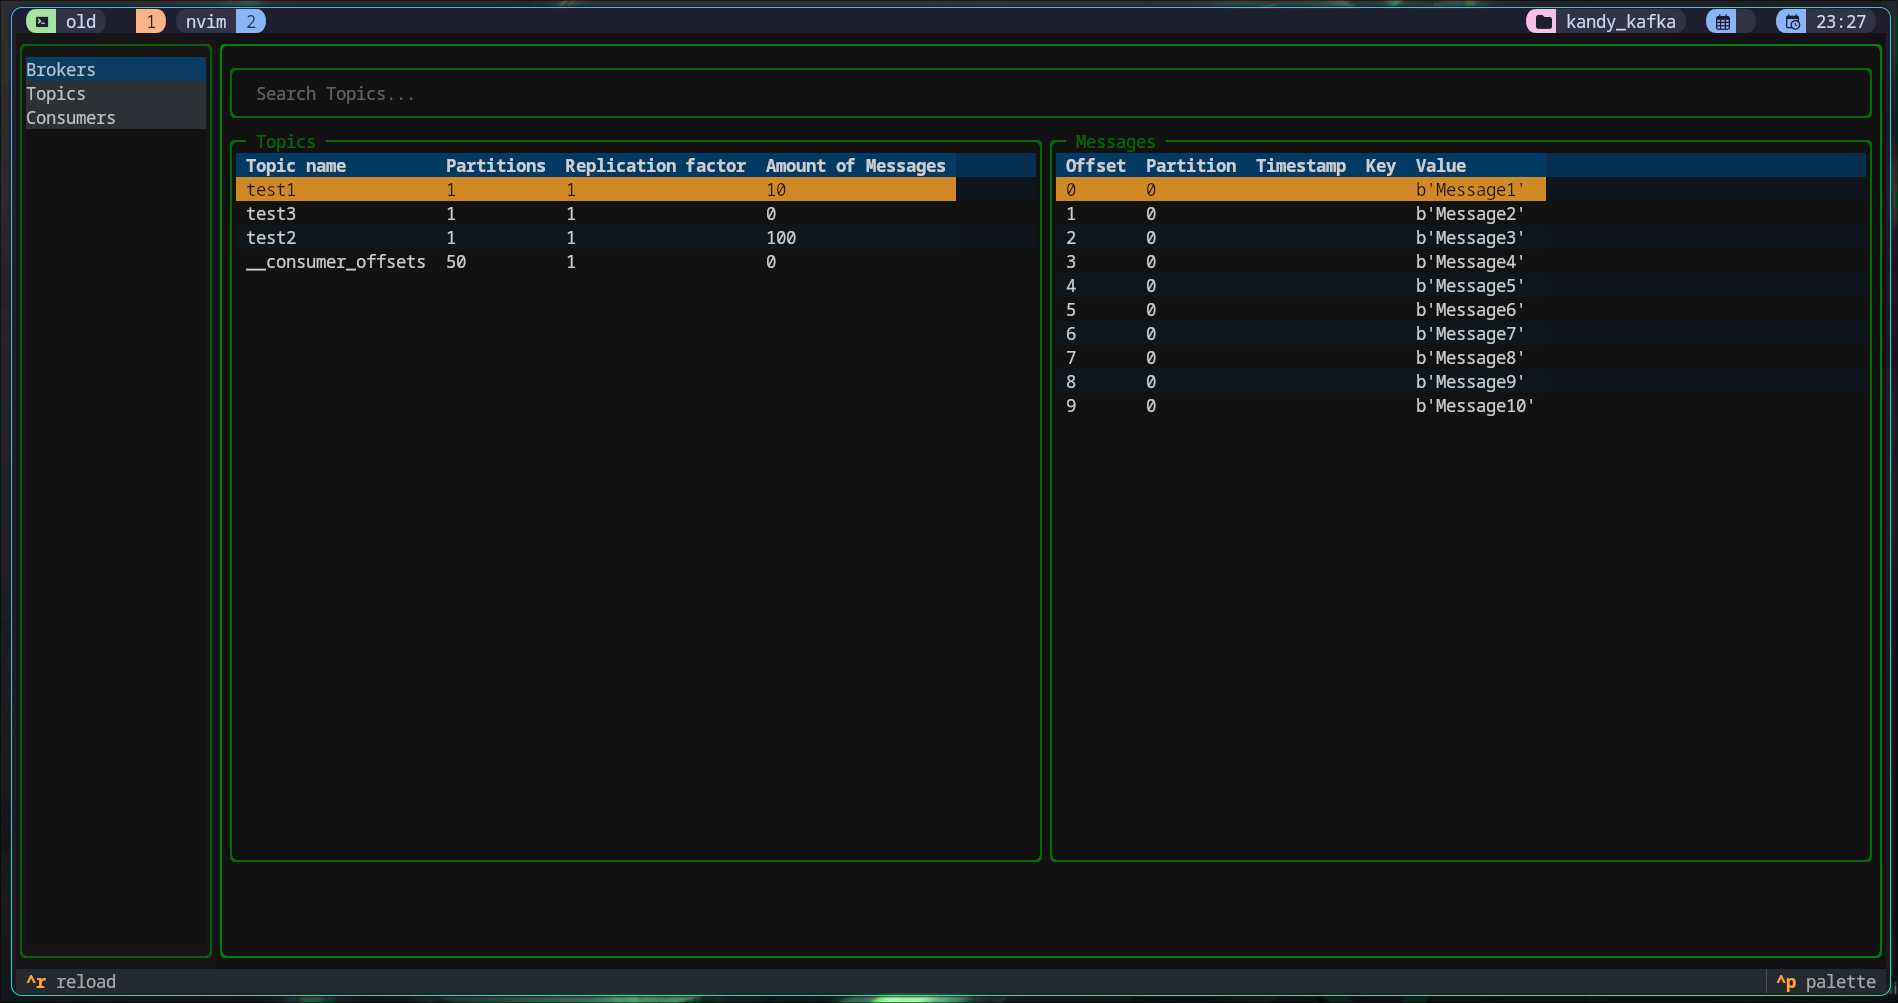
\includegraphics[width=0.95\textwidth]{imgs/FinalUI.png}
  \end{center}
  \caption{}\label{fig:}
\end{figure}

One interesting feature I added is a loading spinner for messages, so users can tell that the application is working and hasn’t frozen. To implement this, part of the functionality had to be made asynchronous, as otherwise, the entire application would hang while fetching messages from a topic, which is clearly unacceptable.

\begin{figure}[htbp]
  \begin{center}
    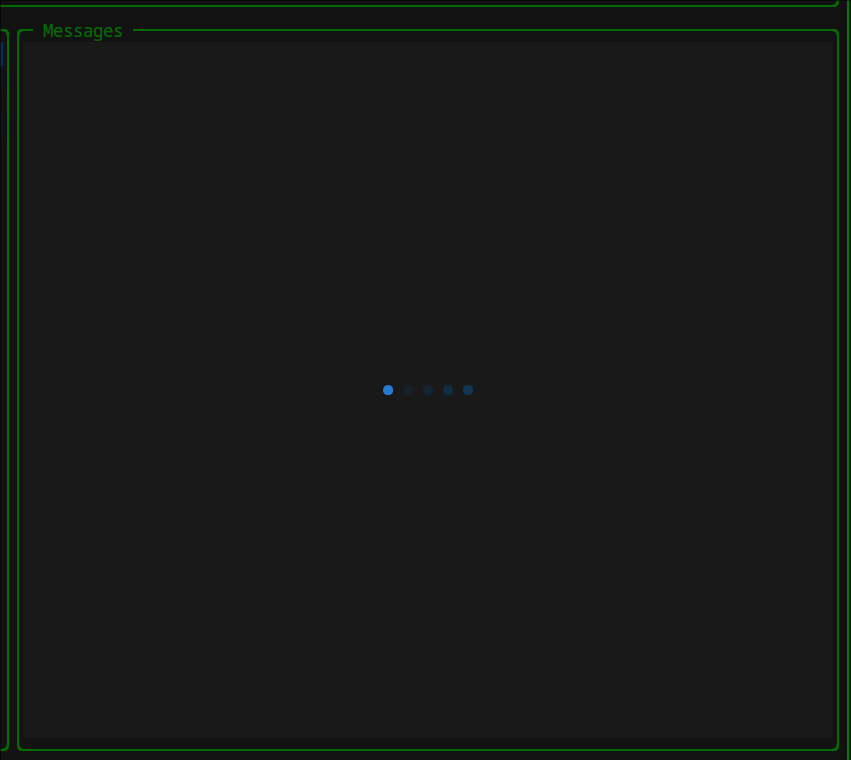
\includegraphics[width=0.95\textwidth]{imgs/MessagesSpinner.png}
  \end{center}
  \caption{}\label{fig:}
\end{figure}

\newpage
\subsection{Comments and annotation}

During the development of the first release, since I changed the code often and the logic was generally not overcomplicated, I was leaving most of the code without any comments and/or annotations, but as the codebase grew, I had to spend more and more time on refactoring, so later versions of the code have more and more comments and the final code that I presented in Appendix~\ref{appendix:project} is fully annotated following PEP8 - Python standards. Each function is described in the docstring using the following template:

\begin{itemize}
\item Purpose: brief explanation of what this function does
\item Arguments: Input of function
\item Return: What does this function return
\end{itemize}

\begin{figure}[htbp]
  \begin{center}
    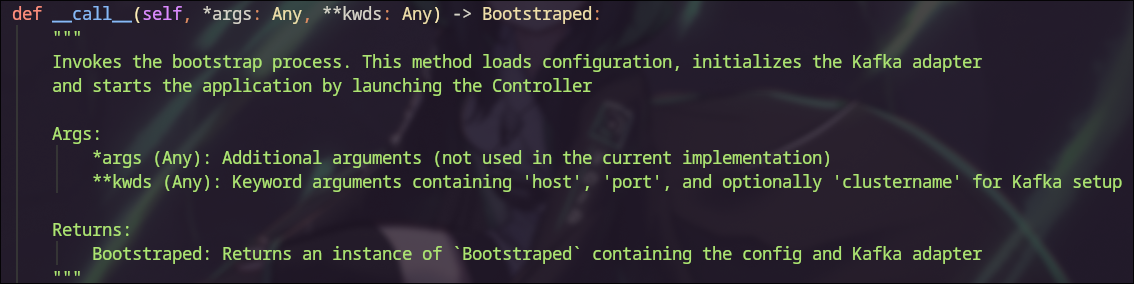
\includegraphics[width=0.95\textwidth]{imgs/DocStringExample.png}
  \end{center}
  \caption{Docstring example}\label{fig:}
\end{figure}


\newpage
\chapter{Evaluation}

\begin{table}[h!tbp]
\centering
\renewcommand{\arraystretch}{1.3}
\begin{adjustbox}{max width=\textwidth}
\begin{tabular}{|p{3.5cm}|p{5.5cm}|p{3.5cm}|p{3.5cm}|}
\hline
\textbf{Criterion} & \textbf{Evidence Summary} & \textbf{Evaluation Result} & \textbf{Explanation} \\ \hline

\textbf{Connecting to Kafka} & 
\texttt{check\_config\_details} test  confirms that valid configuration files allow correct connection details to be loaded. Logs show successful KafkaAdapter initialization. & 
Fully Met & 
The system establishes connections successfully when valid configuration files are provided, fulfilling the criterion. \\ \hline

\textbf{Fetching Topics} & 
No specific test evidence or logs are provided for fetching topics. Bootstrap success suggests topics might be fetched implicitly. & 
Partially Met & 
The absence of explicit logs or tests leaves uncertainty regarding topic-fetching behavior. Additional tests are needed to verify performance within defined limits. \\ \hline

\textbf{Fetching Messages} & 
Logs confirm that messages are fetched successfully, with offsets tracked and polling completed within 10 seconds (\texttt{kafka\_adapter.py:85, 151}). & 
Fully Met & 
The system retrieves the 50 oldest messages per topic within the required time frame. \\ \hline

\textbf{Sorting Topics} & 
No tests or logs exist for sorting functionality. Lack of understanding of sorting implementation prevented testing. & 
Fully Unmet & 
Sorting functionality was neither tested nor verified, highlighting a need for future focus on this area. \\ \hline

\textbf{Input Validation} & 
Tests confirm \texttt{HostsFileNotFound} is raised for missing configuration files, and \texttt{HostsFileHasWrongSyntax} is raised for syntax errors. No evidence exists for CLI input validation. & 
Fully Met & 
Configuration validation is well-handled, but CLI input validation remains tested by hand, not script. \\ \hline

\textbf{UI Responsiveness} & 
No specific evidence for UI responsiveness is provided. Indirectly inferred from message-fetching logs showing timely completion. & 
Partially Met & 
Explicit evidence for UI responsiveness is missing. Future tests should include automated UI testing or manual validation logs. \\ \hline

\end{tabular}
\end{adjustbox}
\caption{Evaluation of Initial Success Criteria Based on Test Evidence}
\label{tab:success-evaluation}
\end{table}

\newpage
\subsubsection{Test Evidences:}

\begin{code}
  \begin{minted}{Python}
# Correct syntax scenario
@pytest.fixture
@given("Configuration file has valid syntax")
def config_file_with_correct_syntax(config_file):
    config_file.write_text(
        """
        default:
            host: localhost
            port: 9092
        """
    )


@then("config should have valid connection details")
def check_config_details(config, config_file):
    config.load_hosts("default", config_file)
    assert config.KAFKA_HOST == "localhost"
    assert config.KAFKA_PORT == 9092
\end{minted}
\caption{Input validation and connecting to kafka success criterias}
\end{code}

\begin{figure}[htbp]
  \begin{center}
    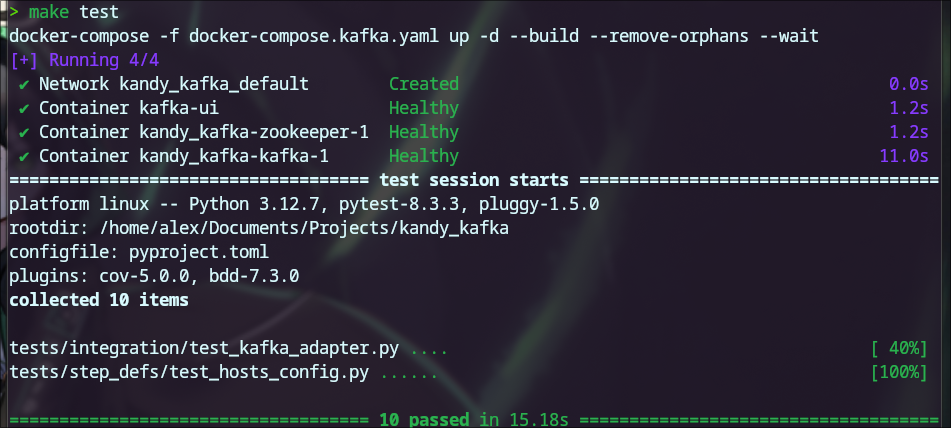
\includegraphics[width=0.95\textwidth]{imgs/FinalTestData.png}
  \end{center}
  \caption{All tests have passed}\label{fig:}
\end{figure}

\begin{code}
  \begin{minted}{text}  
2024-10-21:11:53:47,797 INFO     [bootstrap.py:26] ATTEMPTING TO BOOTSTRAP - creating KafkaAdapter
2024-10-21:11:53:49,508 INFO     [topics.py:191] Loading messages
2024-10-21:11:53:49,508 INFO     [kafka_adapter.py:85] Start polling messages
2024-10-21:11:53:49,524 INFO     [kafka_adapter.py:103] Partition 0: Low: 0, High: 81
2024-10-21:11:53:53,82 INFO     [kafka_adapter.py:151] Reached limit of 50 messages. Stopping.
2024-10-21:11:53:53,82 INFO     [kafka_adapter.py:155] End polling messages for topic: test-topic-wxvlkd
2024-10-21:11:53:53,82 INFO     [topics.py:193] Got messages
2024-10-21:11:57:42,381 INFO     [topics.py:191] Loading messages
2024-10-21:11:57:42,381 INFO     [kafka_adapter.py:85] Start polling messages
2024-10-21:11:57:42,636 INFO     [kafka_adapter.py:103] Partition 0: Low: 0, High: 0
2024-10-21:11:57:42,644 INFO     [kafka_adapter.py:103] Partition 1: Low: 0, High: 0
2024-10-21:11:57:42,647 INFO     [kafka_adapter.py:103] Partition 2: Low: 0, High: 0
2024-10-21:11:57:42,649 INFO     [kafka_adapter.py:103] Partition 3: Low: 0, High: 0
2024-10-21:11:57:42,651 INFO     [kafka_adapter.py:103] Partition 4: Low: 0, High: 0
2024-10-21:11:57:42,654 INFO     [kafka_adapter.py:103] Partition 5: Low: 0, High: 36
2024-10-21:11:57:42,657 INFO     [kafka_adapter.py:103] Partition 6: Low: 0, High: 0
2024-10-21:11:57:42,659 INFO     [kafka_adapter.py:103] Partition 7: Low: 0, High: 0
2024-10-21:11:57:42,662 INFO     [kafka_adapter.py:103] Partition 8: Low: 0, High: 0
2024-10-21:11:57:42,664 INFO     [kafka_adapter.py:103] Partition 9: Low: 0, High: 0
2024-10-21:11:57:42,667 INFO     [kafka_adapter.py:103] Partition 10: Low: 0, High: 0
2024-10-21:11:57:42,669 INFO     [kafka_adapter.py:103] Partition 11: Low: 0, High: 0
2024-10-21:11:57:42,671 INFO     [kafka_adapter.py:103] Partition 12: Low: 0, High: 0
2024-10-21:11:57:42,674 INFO     [kafka_adapter.py:103] Partition 13: Low: 0, High: 0
2024-10-21:11:57:42,674 INFO     [kafka_adapter.py:103] Partition 14: Low: 0, High: 0
2024-10-21:11:57:42,675 INFO     [kafka_adapter.py:103] Partition 15: Low: 0, High: 0
2024-10-21:11:57:42,675 INFO     [kafka_adapter.py:103] Partition 16: Low: 0, High: 0
2024-10-21:11:57:42,676 INFO     [kafka_adapter.py:103] Partition 17: Low: 0, High: 0
2024-10-21:11:57:42,676 INFO     [kafka_adapter.py:103] Partition 18: Low: 0, High: 0
2024-10-21:11:57:42,676 INFO     [kafka_adapter.py:103] Partition 19: Low: 0, High: 0
2024-10-21:11:57:42,676 INFO     [kafka_adapter.py:103] Partition 20: Low: 0, High: 0
2024-10-21:11:57:42,677 INFO     [kafka_adapter.py:103] Partition 21: Low: 0, High: 0
2024-10-21:11:57:42,677 INFO     [kafka_adapter.py:103] Partition 22: Low: 0, High: 0
2024-10-21:11:57:42,677 INFO     [kafka_adapter.py:103] Partition 23: Low: 0, High: 0
2024-10-21:11:57:42,677 INFO     [kafka_adapter.py:103] Partition 24: Low: 0, High: 0
2024-10-21:11:57:42,678 INFO     [kafka_adapter.py:103] Partition 25: Low: 0, High: 0
2024-10-21:11:57:42,678 INFO     [kafka_adapter.py:103] Partition 26: Low: 0, High: 0
2024-10-21:11:57:42,678 INFO     [kafka_adapter.py:103] Partition 27: Low: 0, High: 0
2024-10-21:11:57:42,678 INFO     [kafka_adapter.py:103] Partition 28: Low: 0, High: 0
2024-10-21:11:57:42,679 INFO     [kafka_adapter.py:103] Partition 29: Low: 0, High: 0
2024-10-21:11:57:42,679 INFO     [kafka_adapter.py:103] Partition 30: Low: 0, High: 0
2024-10-21:11:57:42,679 INFO     [kafka_adapter.py:103] Partition 31: Low: 0, High: 0
2024-10-21:11:57:42,679 INFO     [kafka_adapter.py:103] Partition 32: Low: 0, High: 0
2024-10-21:11:57:42,680 INFO     [kafka_adapter.py:103] Partition 33: Low: 0, High: 0
2024-10-21:11:57:42,680 INFO     [kafka_adapter.py:103] Partition 34: Low: 0, High: 0
2024-10-21:11:57:42,680 INFO     [kafka_adapter.py:103] Partition 35: Low: 0, High: 0
2024-10-21:11:57:42,681 INFO     [kafka_adapter.py:103] Partition 36: Low: 0, High: 0
2024-10-21:11:57:42,681 INFO     [kafka_adapter.py:103] Partition 37: Low: 0, High: 0
2024-10-21:11:57:42,682 INFO     [kafka_adapter.py:103] Partition 38: Low: 0, High: 0
2024-10-21:11:57:42,682 INFO     [kafka_adapter.py:103] Partition 39: Low: 0, High: 0
2024-10-21:11:57:42,682 INFO     [kafka_adapter.py:103] Partition 40: Low: 0, High: 0
2024-10-21:11:57:42,683 INFO     [kafka_adapter.py:103] Partition 41: Low: 0, High: 0
2024-10-21:11:57:42,683 INFO     [kafka_adapter.py:103] Partition 42: Low: 0, High: 0
2024-10-21:11:57:42,683 INFO     [kafka_adapter.py:103] Partition 43: Low: 0, High: 0
2024-10-21:11:57:42,684 INFO     [kafka_adapter.py:103] Partition 44: Low: 0, High: 0
2024-10-21:11:57:42,684 INFO     [kafka_adapter.py:103] Partition 45: Low: 0, High: 0
2024-10-21:11:57:42,684 INFO     [kafka_adapter.py:103] Partition 46: Low: 0, High: 0
2024-10-21:11:57:42,685 INFO     [kafka_adapter.py:103] Partition 47: Low: 0, High: 0
2024-10-21:11:57:42,685 INFO     [kafka_adapter.py:103] Partition 48: Low: 0, High: 0
2024-10-21:11:57:42,685 INFO     [kafka_adapter.py:103] Partition 49: Low: 0, High: 0
2024-10-21:11:57:44,259 INFO     [kafka_adapter.py:118] All partitions have been fully consumed. Stopping.
2024-10-21:11:57:44,259 INFO     [kafka_adapter.py:155] End polling messages for topic: __consumer_offsets
2024-10-21:11:57:44,259 INFO     [topics.py:193] Got messages
2024-10-21:11:57:53,325 INFO     [bootstrap.py:38] BOOTSTRAPING Completed
2024-10-21:12:17:02,186 INFO     [bootstrap.py:26] ATTEMPTING TO BOOTSTRAP - creating KafkaAdapter
  \end{minted}
  \caption{kandy.log}
\end{code}

\newpage
\subsection{Addressing Partially Met and Unmet Criteria}

The table below outlines the partially met and unmet success criteria, the issues identified, and the proposed solutions for addressing these in future development.

\begin{table}[h!tbp]
\centering
\renewcommand{\arraystretch}{1.3}
\begin{adjustbox}{max width=\textwidth}
\begin{tabular}{|p{3.5cm}|p{6.5cm}|p{5.5cm}|}
\hline
\textbf{Criterion} & \textbf{Issue} & \textbf{Proposed Solution} \\ \hline

\textbf{Sorting Topics} & 
Sorting functionality was not tested due to a lack of understanding of the implementation of tests. &
\begin{itemize}
  \item Learn how to write tests for textual UI
  \item Learn to make proper benchmark tests
\end{itemize} \\ \hline

\textbf{UI Responsiveness} & 
No direct evidence of UI responsiveness; inferred only from timely message-fetching logs. &
\begin{itemize}
    \item Implement automated UI tests using tools like Selenium or Playwright to simulate user interactions.
    \item Log UI transitions (e.g., fetching messages or sorting topics) to confirm responsiveness.
    \item Conduct manual stress testing with large datasets to identify bottlenecks.
    \item Invite stakeholders to test UI; Unfortunately I didn't have such opportuinity, as I chose stakehoder without considering their availability for interviews
\end{itemize} \\ \hline

\end{tabular}
\end{adjustbox}
\caption{Addressing Partially Met and Unmet Criteria}
\label{tab:addressing-criteria}
\end{table}

\newpage
\subsection{Maintenance Issues and Limitations of the Solution}

The following section outlines the key maintenance challenges and limitations identified in the current solution, along with proposed solutions for addressing these issues in future development.

\subsubsection{Configuration Management}
The current approach relies on manually created and maintained configuration files. This introduces a risk of user errors, such as syntax mistakes or missing fields, which can disrupt system functionality.

\textbf{Proposed Solutions:}
\begin{itemize}
    \item Implement a user-friendly configuration wizard to guide users through creating and validating configuration files.
\end{itemize}

\subsubsection{Testing Coverage}
The sorting functionality remains untested due to a lack of understanding of how to implement relevant tests. This limits confidence in its correctness and performance. Only solution I have is to learn harder and budgget more time for testing

\subsubsection{Scalability}
The current solution assumes small-to-medium Kafka clusters, but it may face performance issues when handling larger datasets. Fetching messages or topics could become bottlenecks, to address this issues I have to 

\begin{itemize}
    \item Optimize message-fetching and sorting algorithms to handle large Kafka topics efficiently.
    \item Introduce mechanisms like pagination or streaming for handling large datasets incrementally.
\end{itemize}

\subsubsection{Error Handling}
Errors, such as invalid CLI inputs or corrupted configuration files, are currently raised but often lack actionable feedback for the user. Also I couldn't find any information on how to deal with confluent\_kafka lib errors, which are directly stramed to stdout


\subsubsection{UI Responsiveness}
UI responsiveness is inferred rather than explicitly tested, raising concerns about its behavior under heavy loads or large datasets.

\textbf{Proposed Solutions:}
\begin{itemize}
    \item Implement performance profiling for key UI actions under different load conditions.
    \item Optimize UI updates to prioritize responsiveness during intensive Kafka operations.
\end{itemize}


\subsubsection{Documentation}
Whole application lack detailed documentation, despite having detailed comments. This gap can impede future development and maintenance efforts. There is only one solution - do actualy write documentation


\newpage
\appendix
\chapter{System Design}\label{appendix:system_design}
\begin{figure}[htpb]
    \centering
    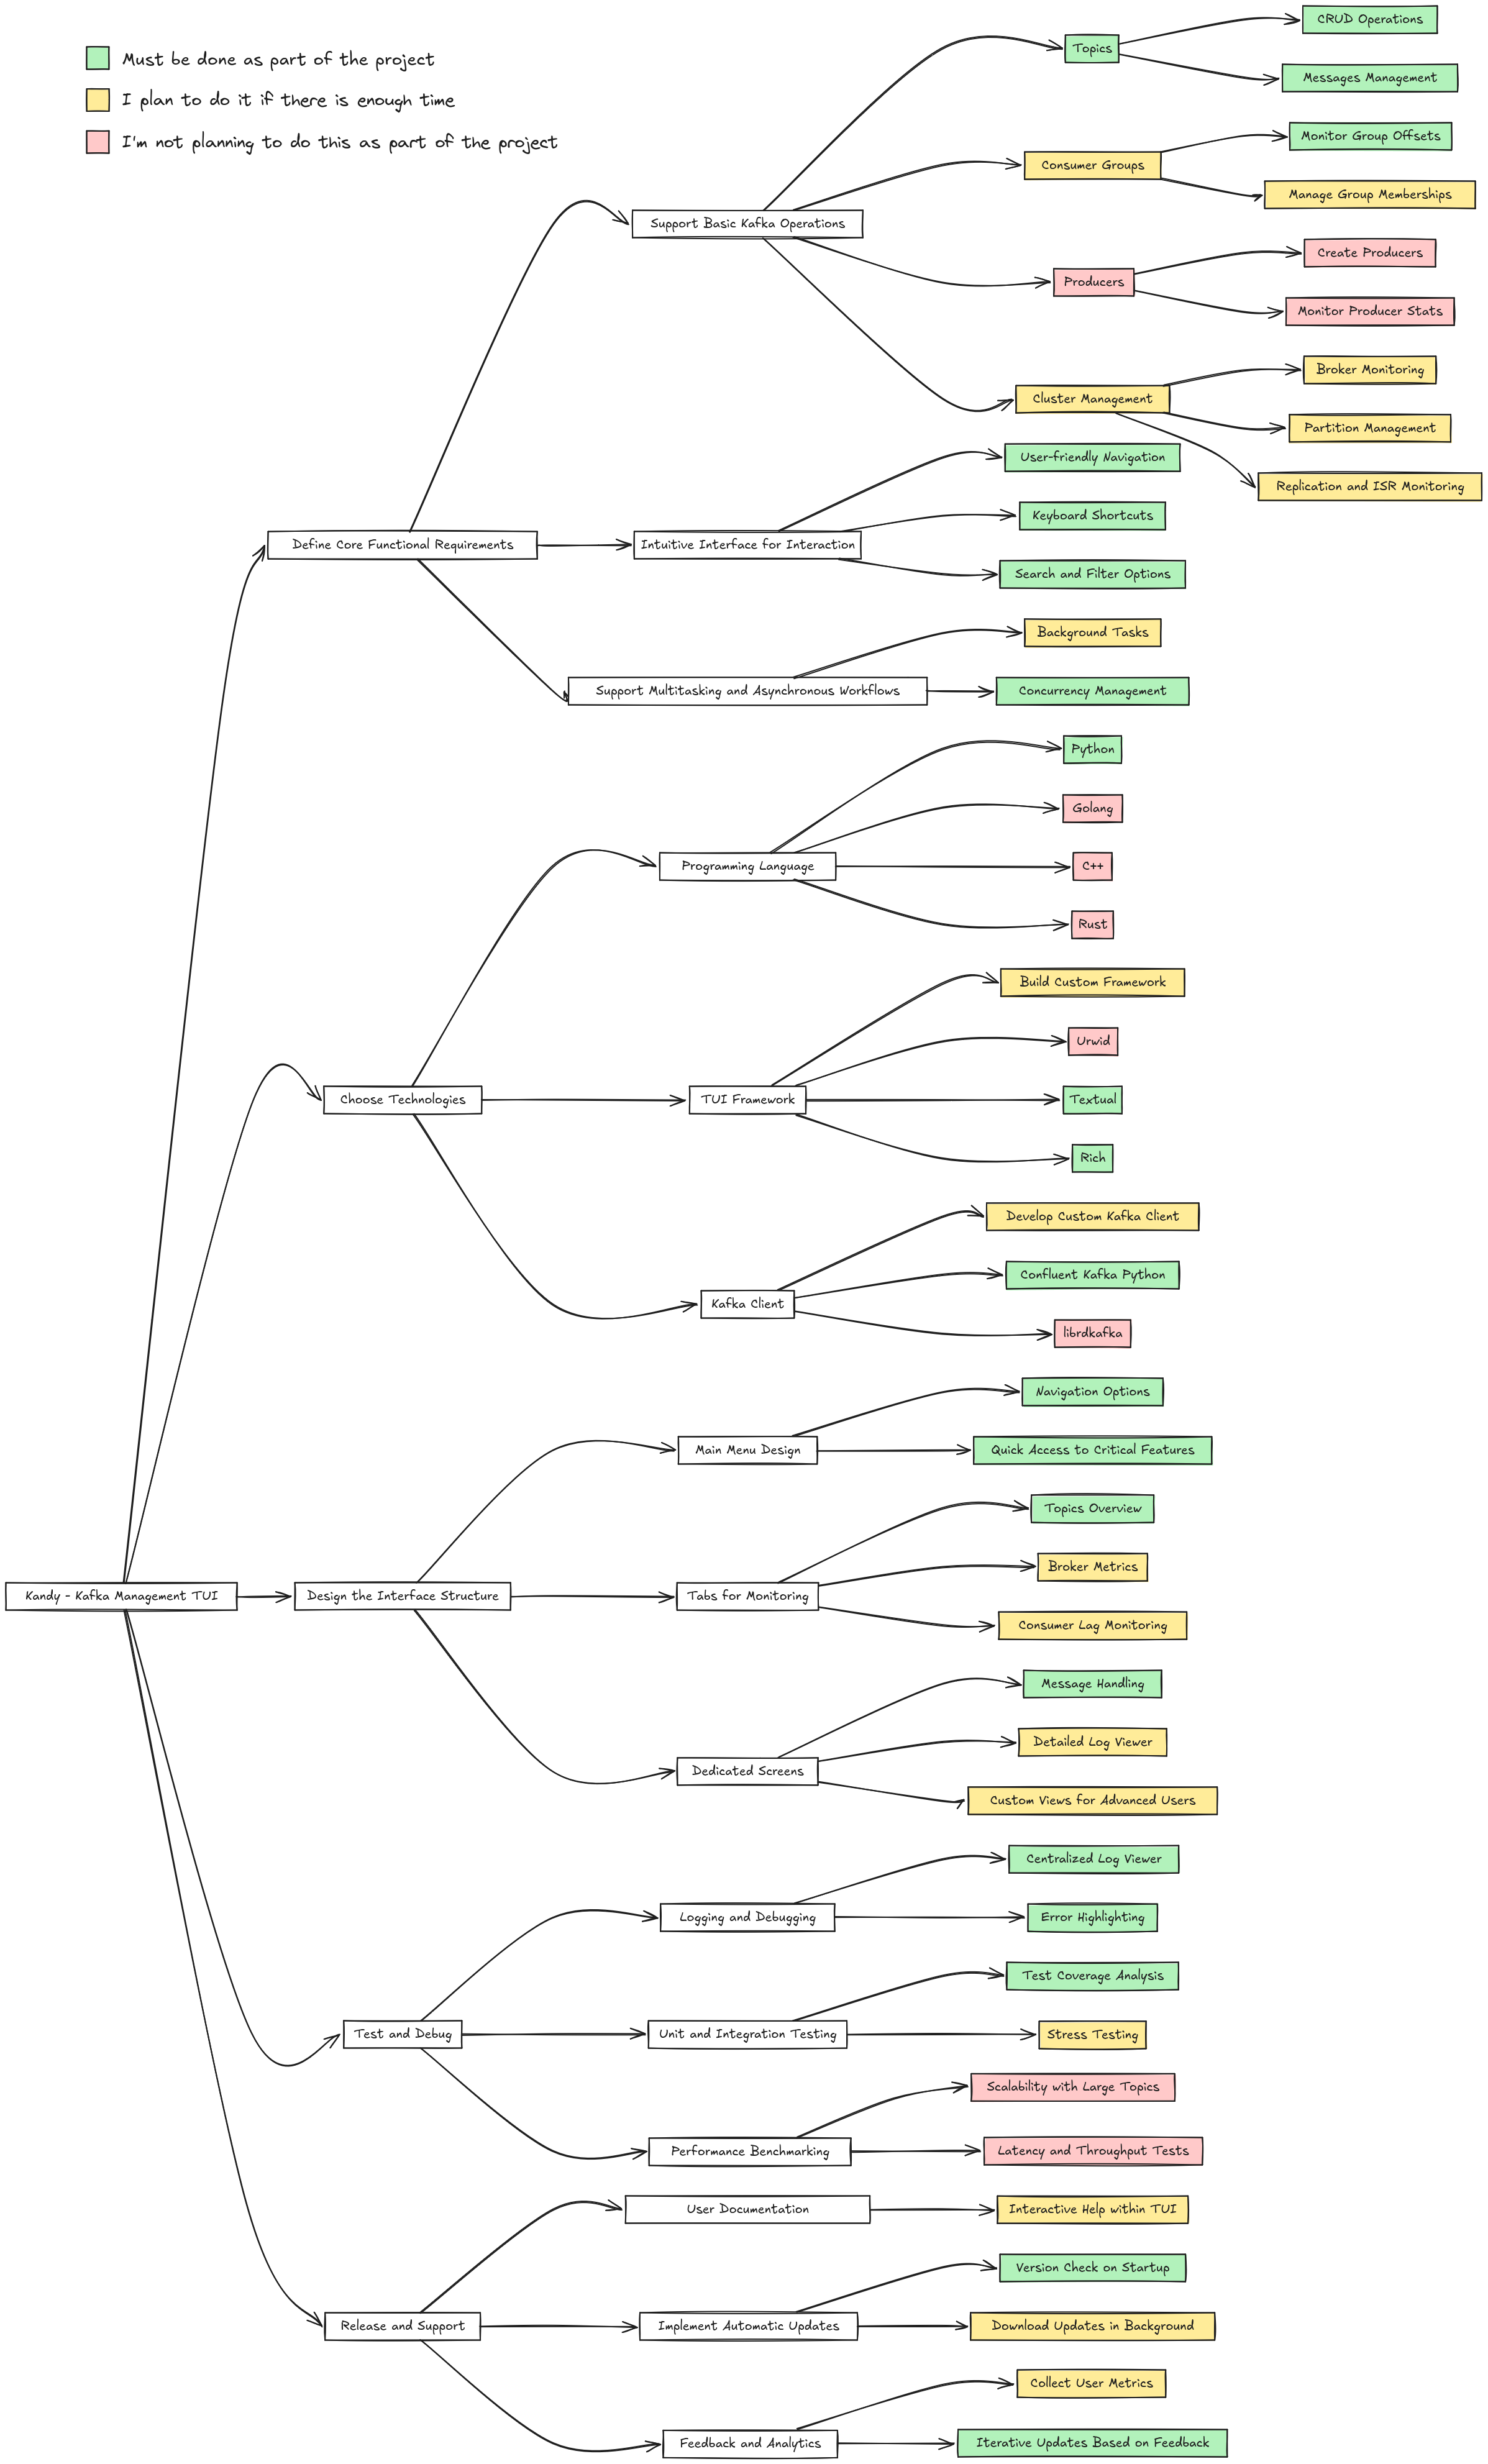
\includegraphics[width=0.7\linewidth]{imgs/SystemDesign.png}
\end{figure}

\chapter{Files}
\section{pyproject.toml (Libraries and dependencies)}\label{appendix:libs}
\begin{listing}[htbp]
    \begin{minted}{Python}
[tool.poetry]
name = "kandy-kafka"
version = "0.0.1"
description = "Handy way to manage kafka"
authors = ["Perchinka <alexsator.lukin@gmail.com>"]
license = "GPL-2.0-only"
readme = "README.md"

[tool.poetry.dependencies]
python = "^3.11"
confluent-kafka = "^2.3.0"
urwid = "^2.6.10"
panwid = "^0.3.5"
pydantic = "^2.6.4"
pyyaml = "^6.0.1"
textual = "^0.81.0"

[tool.poetry.dev-dependencies]
pytest = "^8.1.1"
pytest-bdd = "^7.1.2"
pytest-cov = "^5.0.0"

[build-system]
requires = ["poetry-core"]
build-backend = "poetry.core.masonry.api"
    \end{minted}
    \caption{pyproject.toml}
\end{listing}

\newpage
\section{Project}\label{appendix:project}
\subsection{Structer}
\begin{figure}[htbp]
\centering
  \begin{small}
    \begin{BVerbatim}
.
├── kandy_kafka
│   ├── adapters
│   │   ├── __init__.py
│   │   └── kafka_adapter.py
│   ├── domain
│   │   ├── __init__.py
│   │   └── models.py
│   ├── entrypoints
│   │   └── __init__.py
│   ├── gui
│   │   ├── app.css
│   │   ├── controller.py
│   │   ├── __init__.py
│   │   └── views
│   │       ├── __init__.py
│   │       └── topics.py
│   ├── exceptions.py
│   ├── bootstrap.py
│   ├── config.py
│   └── logger.py
├── tests
│   ├── conftest.py
│   ├── features
│   │   └── hosts.feature
│   ├── fixtures
│   │   ├── hosts
│   │   │   ├── wrong_syntax_empty_file.yaml
│   │   │   ├── wrong_syntax_missing_host.yaml
│   │   │   └── wrong_syntax_missing_port.yaml
│   │   ├── __init__.py
│   │   ├── kafka_admin.py
│   │   └── kafka_consumer.py
│   ├── integration
│   │   └── test_kafka_adapter.py
│   ├── step_defs
│   │   └── test_hosts_config.py
│   └── unit
│       └── test_hosts_config_fields.py
├── docker-compose.kafka.yaml
├── kandy.py
├── LICENSE
├── Makefile
├── pyproject.toml
└── README.md
      \end{BVerbatim}
    \end{small}
\end{figure}
\newpage

\section{./}
\subsection{docker-compose.kafka.yaml}
\begin{code}
  \inputminted[fontsize=\small]{YAML}{../docker-compose.kafka.yaml}
\end{code}

\subsection{kandy.py}
\begin{code}
  \inputminted[fontsize=\small]{Python}{../kandy.py}
\end{code}

\subsection{Makefile}
\begin{code}
  \inputminted[fontsize=\small]{make}{../Makefile}
\end{code}

\subsection{README.md}
\begin{code}
  \inputminted[fontsize=\small]{MarkDown}{../README.md}
\end{code}

\newpage
\section{./kandy\_kafka}
\subsection{adapters/kafka\_adapter.py}
\begin{code}
  \inputminted[fontsize=\small]{Python}{../kandy_kafka/adapters/kafka_adapter.py}
\end{code}

\subsection{domain/models.py}
\begin{code}
  \inputminted[fontsize=\small]{Python}{../kandy_kafka/domain/models.py}
\end{code}

\subsection{gui/app.css}
\begin{code}
  \inputminted[fontsize=\small]{text}{../kandy_kafka/gui/app.css}
\end{code}

\subsection{gui/controller.py}
\begin{code}
  \inputminted[fontsize=\small]{Python}{../kandy_kafka/gui/controller.py}
\end{code}

\subsection{gui/views/topics.py}
\begin{code}
  \inputminted[fontsize=\small]{Python}{../kandy_kafka/gui/views/topics.py}
\end{code}

\subsection{exceptions.py}
\begin{code}
  \inputminted[fontsize=\small]{Python}{../kandy_kafka/exceptions.py}
\end{code}

\subsection{bootstrap.py}
\begin{code}
  \inputminted[fontsize=\small]{Python}{../kandy_kafka/bootstrap.py}
\end{code}

\subsection{config.py}
\begin{code}
  \inputminted[fontsize=\small]{Python}{../kandy_kafka/config.py}
\end{code}

\subsection{logger.py}
\begin{code}
  \inputminted[fontsize=\small]{Python}{../kandy_kafka/logger.py}
\end{code}

\newpage
\section{./tests}
\subsection{conftest.py}
\begin{code}
  \inputminted[fontsize=\small]{Python}{../tests/conftest.py}
\end{code}

\subsection{features/hosts.feature}
\begin{code}
  \inputminted[fontsize=\small]{Gherkin}{../tests/features/hosts.feature}
\end{code}

\subsection{fixtures/hosts/wrong\_syntax\_empty\_file.yaml}
\begin{code}
  \inputminted[fontsize=\small]{YAML}{../tests/fixtures/hosts/wrong_syntax_empty_file.yaml}
\end{code}

\subsection{fixtures/hosts/wrong\_syntax\_missing\_host.yaml}
\begin{code}
  \inputminted[fontsize=\small]{YAML}{../tests/fixtures/hosts/wrong_syntax_missing_host.yaml}
\end{code}

\subsection{fixtures/hosts/wrong\_syntax\_missing\_port.yaml}
\begin{code}
  \inputminted[fontsize=\small]{YAML}{../tests/fixtures/hosts/wrong_syntax_missing_port.yaml}
\end{code}

\subsection{fixtures/hosts/kafka\_admin.py}
\begin{code}
  \inputminted[fontsize=\small]{Python}{../tests/fixtures/kafka_admin.py}
\end{code}

\subsection{fixtures/hosts/kafka\_consumer.py}
\begin{code}
  \inputminted[fontsize=\small]{Python}{../tests/fixtures/kafka_consumer.py}
\end{code}

\subsection{integration/test\_kafka\_adapter.py}
\begin{code}
  \inputminted[fontsize=\small]{Python}{../tests/integration/test_kafka_adapter.py}
\end{code}

\subsection{step\_defs/test\_hosts\_config.py}
\begin{code}
  \inputminted[fontsize=\small]{Python}{../tests/step_defs/test_hosts_config.py}
\end{code}

\subsection{unit/test\_hosts\_config\_fields.py}
\begin{code}
  \inputminted[fontsize=\small]{Python}{../tests/unit/test_hosts_config_fields.py}
\end{code}

\renewcommand{\bibname}{References}
\begin{thebibliography}{00}
\bibitem{confluent-kafka-docs} docs.confluent.io. (n.d.). confluent\_kafka API — confluent-kafka 2.2.0 documentation. [online] Available at: https://docs.confluent.io/platform/current/clients/confluent-kafka-python/html/index.html.

\bibitem{textual-docs} Textual Documentation. (n.d.). Textual - Tutorial. [online] Available at: https://textual.textualize.io/tutorial/.

\bibitem{urwid-docs} Urwid.org. (2014). — Urwid 2.6.14. [online] Available at: https://urwid.org/index.html [Accessed 10 Dec. 2024].

\bibitem{pydantic-docs} docs.pydantic.dev. (n.d.). Pydantic. [online] Available at: https://docs.pydantic.dev/latest/.

\bibitem{refactor-guru} Refactoring Guru (2014). Design Patterns. [online] Refactoring.guru. Available at: https://refactoring.guru/design-patterns.

\bibitem{source-confluent-kafka} GitHub. (n.d.). GitHub - confluentinc/confluent-kafka-python: Confluent’s Kafka Python Client. [online] Available at: https://github.com/confluentinc/confluent-kafka-python.


\bibitem{b1} Docker.com. (2024). Available at: https://hub.docker.com/r/confluentinc/cp-kafka [Accessed 12 Dec. 2024].

\bibitem{b2} docs.pytest.org. (n.d.). pytest: helps you write better programs — pytest documentation. [online] Available at: https://docs.pytest.org/en/stable/.

\bibitem{b3} pytest-bdd.readthedocs.io. (n.d.). Welcome to Pytest-BDD’s documentation! — Pytest-BDD 7.1.2 documentation. [online] Available at: https://pytest-bdd.readthedocs.io/en/stable/.

\bibitem{b4} jhogan (2024). GitHub - jhogan/pywid: A Python library for creating Curses based widgets. [online] GitHub. Available at: https://github.com/jhogan/pywid/tree/master [Accessed 12 Dec. 2024].

\bibitem{b5} Apache Kafka. (n.d.). Apache Kafka. [online] Available at: https://kafka.apache.org/documentation/.

\bibitem{b6} design-practice-repository. (2016). design-practice-repository. [online] Available at: https://socadk.github.io/design-practice-repository/artifact-templates/DPR-QualityAttributeScenario.html.

\end{thebibliography}

\end{document}
